\documentclass[a4paper,11pt]{report}

% remove runningheads to submit
\usepackage[english]{babel}

% portuguese
\usepackage{graphicx}
\usepackage{float}
\usepackage{array}
\usepackage{listings}
\usepackage{courier}
\usepackage{color}
\usepackage{bnf}
\usepackage{appendix}
\usepackage[boxed,linesnumbered]{algorithm2e}

\lstset{
         basicstyle=\footnotesize\ttfamily, % Standardschrift
         %numbers=left,               % Ort der Zeilennummern
         numberstyle=\tiny,          % Stil der Zeilennummern
         %stepnumber=2,               % Abstand zwischen den Zeilennummern
         numbersep=5pt,              % Abstand der Nummern zum Text
         tabsize=3,                  % Groesse von Tabs
         %extendedchars=true,         %
         breaklines=true,            % Zeilen werden Umgebrochen
         keywordstyle=\color{red},
                %frame=b,         
 %        keywordstyle=[1]\textbf,    % Stil der Keywords
 %        keywordstyle=[2]\textbf,    %
 %        keywordstyle=[3]\textbf,    %
 %        keywordstyle=[4]\textbf,   \sqrt{\sqrt{}} %
         %stringstyle=\color{white}\ttfamily, % Farbe der String
         showspaces=false,           % Leerzeichen anzeigen ?
         showtabs=false,             % Tabs anzeigen ?
         xleftmargin=10pt,
         framexleftmargin=5pt,
         framexrightmargin=10pt,
         framexbottommargin=4pt,
         %backgroundcolor=\color{lightgray},
         %showstringspaces=false      % Leerzeichen in Strings anzeigen ?        
 }
 

\usepackage{caption}
\DeclareCaptionFont{blue}{\color{blue}} 
   \captionsetup[lstlisting]{singlelinecheck=false, labelfont={blue}, textfont={blue}}
   
 \DeclareCaptionFont{white}{\color{white}}
 \DeclareCaptionFormat{listing}{\colorbox[cmyk]{0.43, 0.35, 0.35,0.01}{\parbox{\textwidth}{\hspace{15pt}#1#2#3}}}
\captionsetup[lstlisting]{format=listing,labelfont=white,textfont=white, singlelinecheck=false, margin=-2pt, font={bf,footnotesize}}

% images: .png or .pdf w/ pdflatex; .eps w/ latex
\usepackage[latin1]{inputenc}

\usepackage[hyphens]{url}

% urls
%\usepackage{times}

% PS fonts
%\usepackage[T1]{fontenc}
\usepackage{a4wide}

%\hyphenation{}                  % explicit hyphenation
% entities
%\newcommand{\class}[1]{{\normalfont\slshape #1\/}}
\begin{document}
\title{BioSeD - \textbf{Bio}logical \textbf{Se}quences \textbf{D}atabase}

\author{Fl�vio Manuel Fernandes Cruz \\ Instituto de Biologia Molecular, R.\ do Campo Alegre, 823\\4150-180 Porto.\\
\textbf{flaviocruz.net - ei05011@fe.up.pt}}

%\institute{Instituto de Biologia Molecular, R.\ do Campo Alegre, 823\\4150-180 Porto.\\
%\email{flaviocruz.net}\\
%\email{ei05011@fe.up.pt}}
\date{\today}


\maketitle


\addcontentsline{toc}{chapter}{Contents}
\tableofcontents
\listoffigures
\listoftables
\lstlistoflistings
\listofalgorithms
\clearpage

\chapter{Introduction}\label{sec:introduction}

This report describes the design and implementation of a computer system that was built
to store sequences and related annotations.

We designed a flexible system where it is possible to:
attach an arbitrary number of annotations (which we call \textit{labels})
to a sequence; have different kinds of labels; make automatic annotations when
a sequence is added into the system or is modified; and, mainly,
to make arbitrarily complex search queries using annotated information.
Efficient search of sequences by some specific characteristics is then,
the main objective of the system and its crucial functionality.

During sequence search it is possible to apply operations to the whole result list,
such as: add new labels, delete current labels, change label
values, export the sequence list, do a BLAST search on the result set,
and translate the result list using annotated
information. This last functionality makes possible to retrieve the protein sequences
from a set of DNA sequences.

Each label stored in the system has properties that define its behavior.
Some of properties include: if the label should be
auto generated when a sequence is added; if it is user editable or deletable; 
and the code used to generate annotations using a sequence as input.

The system supports basic label types such as: integer, float, boolean,
simple text, date, url, a sequence position, reference to a sequence, a file
(basically the same as attaching files to a sequence) and a reference to a taxonomy.

Another important facility is the use of taxonomies.
The system is able to store multiple taxonomy trees and annotate sequences
with labels that act as references to taxonomies. The basic use case of this
functionality is the creation of a label named \textit{species}, which annotates each
sequence with the corresponding species.

The NCBI taxonomy tree is present by default, but the system allows the creation of new and custom taxonomy trees.

Every data stored is exportable and importable, to and from files.
The system adopts the FASTA, XML and CSV formats to export sequences and related annotations.
The XML format is used to export everything else.

The system, implemented as a web application, uses the client/server design architecture.
Some features, like searching and data viewing, can be used without client authentication, but
everything else requires authentication.
Some clients can be application administrators and have the permission to edit user information, manage labels and do database maintenance.

The rest of the report is organized as follows. First, we analyze some systems that try to do the same as ours.
We will describe the advantages, faults and the flexibility of those systems. Next, we describe more thoroughly each system object, the sequence, the label and the taxonomy. With these objects in mind, we describe the design we come up with that tries to maximize flexibility and efficiency. The main object of analysis at this stage is the relational database we implemented to support the features. Following the design we describe some implementation details worth mentioning: the authentication system, how the label code is stored, how we generate the default label values, how do we transform the queries into SQL code and how we parse complex text queries into a manageable format. Next, we describe important user interface elements, like the search, BLAST search and taxonomy tree browsing interfaces. Then we show time results for search operations to analyze the efficiency of the solution. Finally we describe the major difficulties, the future work and the project conclusions.

\clearpage
\chapter{Related Work}

In this section we give an overview of some software systems that support sequence
annotation and searching, and thus, are similar to the system we have implemented.

\section{Genotator}

Developed by Nomi Harris, Genotator \cite{genotator} (formerly known as Genotater) is an annotation workbench consisting
of a program that runs various sequence analysis programs, and a standalone annotation browser.

The goal of Genotator is to run a series of sequence analysis tools and display the results in such a way that
various predictions can be compared. The user will then be able to examine all the annotations and select
the ones that look the best. Useful annotations include homologies to known genes, possible gene locations,
gene signals such as promoters, etc \cite{about_genotator}.

The Genotator back end runs several gene finders, homology searches (using blast), and signal searches and saves the results in .ace format. Genotator thus automates the tedious process of running a dozen different sequence analysis programs with a dozen different input and output formats.

Two displays are supplied: the map display (Figure \ref{fig:genotator}), where the annotations are shown, and the sequence display.
The application can also search a sequence for specific patterns using regular expressions, when in the sequence
display.

Like BioSeD, Genotator can generate sequence annotations, although it fails to provide an
integrated search environment over a set of sequences.

\begin{figure}[ht]
  \centering
    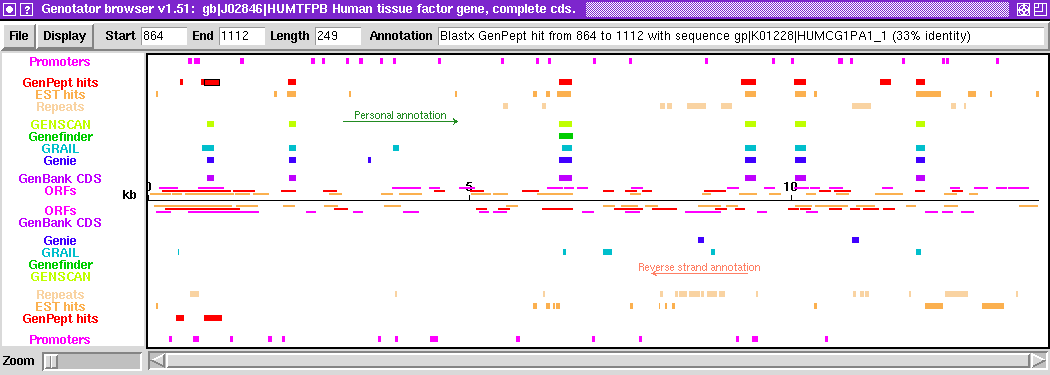
\includegraphics[scale=0.4]{genotator.png}
  \caption{Genotator map view.}
  \label{fig:genotator}
\end{figure}

\section{BioDAS}

The Bio Distributed Annotation System (BioDAS \cite{biodas}) defines a communication protocol used
to exchange annotations on genomic or protein sequences. It is motivated by the idea that such
annotations should not be provided by single centralized databases, but should instead be spread
over multiple sites. Data distribution, performed by DAS servers, is separated from visualization,
which is done by DAS clients. The advantages of this system are that control over the data is
retained by data providers, data is freed from the constraints of specific organizations and the
normal issues of release cycles, API updates and data duplication are avoided. \cite{about_biodas}

DAS is a client-server system in which a single client integrates information from multiple servers.
It allows a single machine to gather up sequence annotation information from multiple distant web sites,
collate the information, and display it to the user in a single view. Little coordination is needed
among the various information providers.
Some well known DAS clients are: Ensembl \cite{ensembl}, Gbrowse \cite{gbrowse}, IGB \cite{igb}, etc.

Contrarily to BioDAS, BioSeD works by centralizing the data on a single database, where the clients can
then make use of it through a web interface. One distributed aspect of BioSeD is present in the data exchange facilities,
as they make possible the integration of data from one application into another.
In BioSeD every piece of data must adhere to the supported data formats, as there is no communication protocol.

\section{EnsMart}

The EnsMart system provides a generic data
warehousing solution for fast and flexible querying of large biological
data sets and integration with third-party data and tools.

The system consists of a query-optimized database and interactive, user-friendly interfaces.
A wide variety of complex queries, on various types of annotations, for numerous species are supported.
Users can group and refine biological data according to many criteria, including cross-species analyses, disease links, sequence variations, and expression patterns. Both tabulated list data and biological sequence output can be generated dynamically, in HTML, text, Microsoft Excel, and compressed formats.

The EnsMart database can be accessed via a public web site (like BioSeD), or through a
Java application suite. Both implementations and the database are
available for local installation, and can be extended to custom data sets. \cite{ensmart}

The EnsMart query process operates in three steps: select a genome focus, filter these 
by criteria, and output formatted results. First select the primary result of interest: species 
genome and its gene, EST gene or SNP contents. Next, filter the available set of these to 
satisfy specific questions, by choosing criteria among genome region, known genes or user- 
specified lists of gene ID, where these are expressed in anatomy and development stage, 
homology to other species, protein domains and SNP attributes. Finally decide on results 
output of features, structures, SNPs, and sequences, including IDs from Ensembl and many 
other databases, protein and microarray attributes, disease associations,
species homologies,as well as file formats suited to spreadsheets, database
or other uses. \cite{ensmart_shopping}

Using various data sets for sequence annotation querying, ease of use
and customizability are the main advantages of this system.

The search process in EnsSmart is very similar to the one present in BioSeD,
but queries in our system can be potentially more complex and arbitrary. Also,
the annotation information in BioSeD is more expansible and flexible, allowing a wide
variety of annotation information.

More recently, the project was renamed to BioMart, but core functionalities are still the same. \cite{biomart}

\section{CBS Genome Atlas Database} 

The CBS \cite{cbs} project provides a filesystem based database for genomic data.
Everything is organized in the filesystem by directories: kingdom/genus/species/strain/segment.
In each directory the system puts basic information like: the FASTA file, 
all protein sequences derived from the GenBank annotation, etc.
They also have a set of Makefile's that are used to generate various sequence annotation values.

To visualize these data, they constructed different types of chromosomal maps (atlases)
some of which include the Structural Atlas, Repeat Atlas and Genome Atlas (Figure \ref{fig:cbs}).
Each atlas is available in either vector graphic format (PS) or compressed bitmap (PNG).
The intermediate files used to build these atlas are maintained as well.
For each property calculated, there is a corresponding list of numerical values
calculated for every base pair in the generate.

Simple sequence annotations are put into a MySQL database. Complex data is linked
from the filesystem to the database.

Like BioSeD, the system can then use the annotated information present in the database
to sort and search using those annotated values.
Visualization wise, only generation of histograms based on
a specific type of annotation is available in BioSeD, more complex visualizations of data are simply not available.
The use of the filesystem to
store annotations is not used in our system, as it only stores data in a relational database.

\section{Extensible open source content management systems and frameworks}

Sean Mooney and his group explored the idea of using open source content management
systems and frameworks to handle large biomedical datasets and the deployment of bioanalytic tools.

In the paper \textit{Extensible open source content management systems and frameworks: a solution for many needs of a bioinformatics group} \cite{extensible_open_source} some approaches to the use of this kind of software
in a bioinformatics setting are discussed.

\begin{figure}[ht]
  \centering
    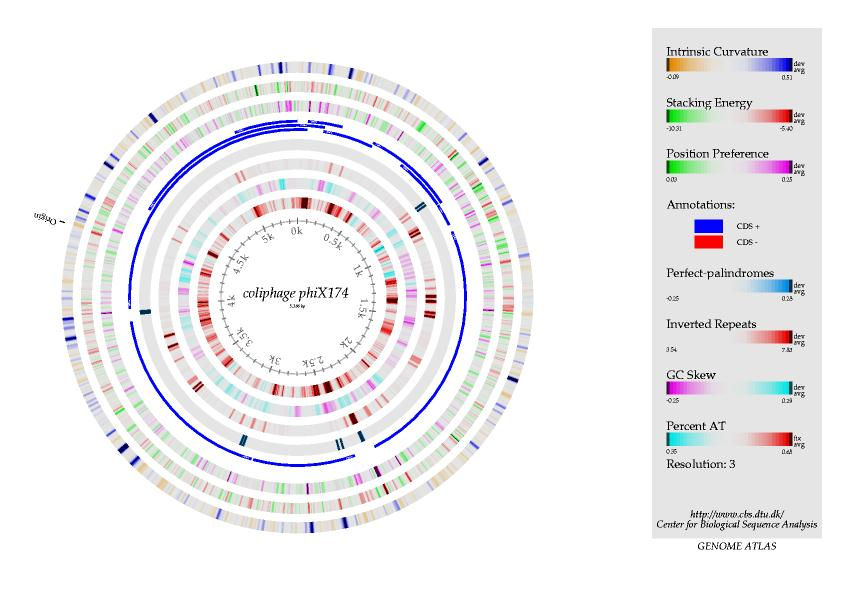
\includegraphics[scale=0.4]{cbs.jpg}
  \caption{The CBS Genome Atlas.}
  \label{fig:cbs}
\end{figure}

\section{GenDB}

GenDB is a genome annotation system for prokaryotic genomes and
supports manual as well as automatic annotation strategies.
It is in use in more than a dozen microbial genome annotation projects.

In addition to its use as a production genome annotation system, it can be employed as a flexible framework for the large-scale evaluation of different annotation strategies.

The GenDB annotation engine will automatically identify, classify and annotate genes using a large collection of software tools, like for example, EMBOSS. BioSeD also supports automatic annotation based on certain events and can also use EMBOSS
or any other tool.

GenDB offers user interfaces that allow expert annotation with large, geo-graphically dispersed teams of experts.
Genes to be annotated can be categorized by functional class or gene location. A number of naming schemes (aka ontologies or functional classification schemes) are supported: GO, TIGR roles, COG, Monica Riley, MIPS. In addition to its use as a production genome annotation system, it can be employed as a flexible framework for the large-scale evaluation of different annotation strategies.

The modular system was developed using an object-oriented approach, and it relies on a relational database backend. Using a well defined application programmers interface (API), the system can be linked easily to other systems. \cite{gendb}
In BioSeD, systems can be linked using data interchange formats or web services using JSON \cite{json}.

\clearpage
\chapter{System objects}\label{sec:objects}

In this section we describe the main system objects: sequence, label, and taxonomy.
Each object will be described by its properties and basic organization.

\section{Sequences}

A \textit{sequence} groups an arbitrary number of label instances, commonly called annotations,
that describe some property of the sequence.
Biologically, a sequence represents a succession of letters forming the primary structure of a
DNA molecule or the structure of a protein.
This succession of letters forms a special label instance named \texttt{content}.
Another basic sequence label is its \texttt{name}.

Each \textit{label instance} is an instance of a label object and
is associated with a specific sequence.
An illustrated sequence is shown in Figure~\ref{fig:seq}.
If a label object named \texttt{length} exists, we can instantiate it
over a set of sequences to represent the corresponding sequence length.

\begin{figure}[H]
  \centering
    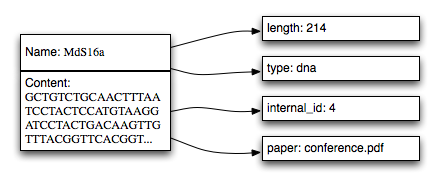
\includegraphics[scale=0.7]{sequence.png}
  \caption{Representation of a sequence object.}
  \label{fig:seq}
\end{figure}

\section{Labels}\label{sec:object_label}

A \textit{label object} represents all the information required to instantiate and manage label instances
over a set of sequences. A label has a set of \textit{label properties} that define its behavior.
The defined properties are described in Table \ref{tbl:label_properties}.

\begin{table}[H]
  \begin{tabular}{ | >{\centering}m{25mm} | >{\centering}m{18mm} | p{11cm} |}
    \hline
    \textbf{Name} & \textbf{Type} & \textbf{Description} \\ \hline
    name & text & The label name. \\ \hline
    type & enum & The label type. \\ \hline
    default & boolean & If true this is a system label and cannot be changed. \\ \hline
    must exist & boolean & If true each sequence must have one instance of this label. \\ \hline
    auto on creation & boolean & If true one instance of this label will be generated using the label code for a newly created sequence. \\ \hline
    auto on modification & boolean & If true and when a sequence content is modified, the corresponding label instance is automatically edited with a new value generated from the label code. \\ \hline
    code & code block & The code used to generate a new label instance. This content is run in the sequence context and may access sequence data like the content.
    The code is in PHP. \\ \hline
    valid code & code block & Code used to validate the label instance. It is also run in the sequence context. \\ \hline
    action modification & code block & Block of code that is run after the sequence's name or content are modified. Useful to implement more specific label properties. \\ \hline
    deletable & boolean & If true the label instances can be user deleted. \\ \hline
    editable & boolean & If true the label instances can be user edited. \\ \hline
    multiple & boolean & If true a sequence can have multiple label instances of the same label. \\ \hline
    public & boolean & If true the label can be used in anonymous searches. \\ \hline
  \end{tabular}
  \caption{Label properties.}
  \label{tbl:label_properties}
\end{table}

Label objects will generate label instances of some \textit{label type} (Table \ref{tbl:label_types}).
The type dictates the data format, the search operators and visualization methods.

\begin{table}[H]
  
  \begin{tabular}{ | >{\centering}m{25mm} | p{11cm} |}
    \hline
    \textbf{Type} & \textbf{Description} \\ \hline
    integer & Simple integer type \\ \hline
    float & Floating point numbers \\ \hline
    text & String of text characters \\ \hline
    object & Whole file: contains the file name and its content \\ \hline
    position & Position in some other sequence: contains the starting position and length \\ \hline
    reference & Reference to some other sequence stored in the system \\ \hline
    taxonomy & Reference to a system's taxonomy \\ \hline
    url & Uniform Resource Locator represented as simple text \\ \hline
    bool & Boolean type \\ \hline
    date & Represents a specific date / time pair \\ \hline
  \end{tabular}
  \caption{Label types.}
  \label{tbl:label_types}
\end{table}

\section{Taxonomies}

It is known that a \textit{taxonomy} classifies another object. By relating sequences and taxonomies,
we can classify some sequence by its originating species or subspecies.

In our system the taxonomy is an object that is linked to a specific \textit{rank} and is aggregated in a \textit{taxonomy tree}.
A tree can have multiple roots.

A name given for each taxonomy is used, system wide, for reference. Unfortunately, it is well known that the same taxonomy can have multiple names for various reasons: commonly used misspellings, synonyms, names used in well known database banks (genbank), etc. To solve this problem, we associate pairs of \textit{secondary names} and reasons for the existence of each taxonomy version.

\begin{figure}[H]
  \centering
    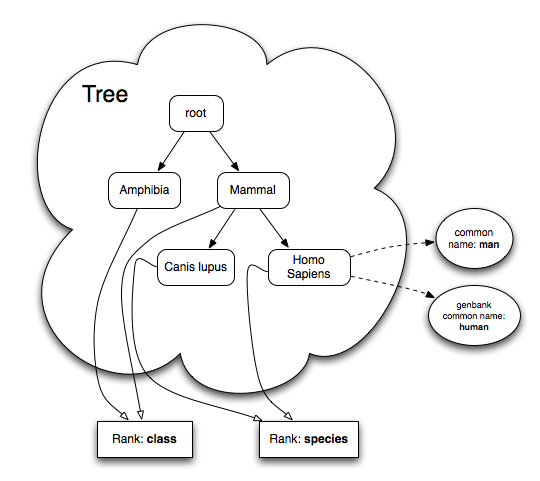
\includegraphics[scale=0.5]{taxonomy.png}
  \caption{A simple taxonomy tree.}
  \label{fig:tax}
\end{figure}

Each taxonomy can be used as label values of the type \textbf{taxonomy} shown in Table \ref{tbl:label_types}.
Figure \ref{fig:tax} shows an example taxonomy tree. The rounded squares represent taxonomies, each taxonomy
points to a squared box representing the specific rank and some taxonomies (in the picture, "Homo Sapiens")
can point to an arbitrary number of secondary names.
An observation should be made: it is recurrent (and natural) that all taxonomies in the same tree level share the same rank.

\clearpage
\chapter{Design}

This section presents the application design and its main components specified. We will start by explaining the top level architecture and how the main system components fit and work together then explaining the designed file formats used throughout the system and the query language specification. 

As we have used a relational database, a relational model will be presented and analyzed. This model will show how the data has been organized to represent objects described in Section \ref{sec:objects} and to make search functionalities more efficient.

\section{Architecture}

The system architecture follows the client/server model very closely (see Figure \ref{fig:architecture}) because it is built as a standard web application. The server hosts the application and delivers HTML pages or JSON objects, through HTTP, to the clients on request. Each client, using a web browser, can access the system and generate new requests based on the current task.

\begin{figure}[H]
  \centering
    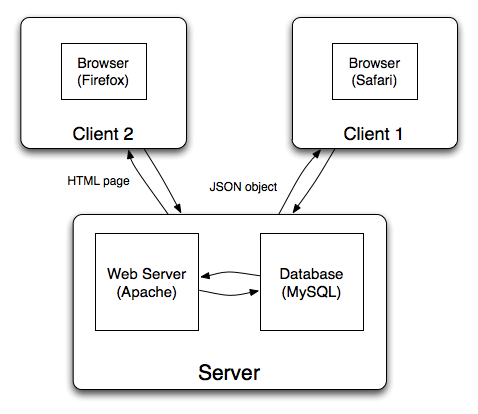
\includegraphics[scale=0.4]{architecture.png}
  \caption{The system top level architecture.}
  \label{fig:architecture}
\end{figure}

\section{Relational Model}

Relational databases are a proven and reliable way of storing relational information. Given this, we designed a database model to store the system objects and everything that is needed to support basic features like user authentication.

\subsection{User tables}

To manage and store user information (Figure~\ref{fig:user_model}) we modeled two tables: the user table (Table \ref{tbl:user_table} on page \pageref{tbl:user_table}) and the configuration table (Table \ref{tbl:configuration_table} on page \pageref{tbl:configuration_table}).
Each row in the user table represents an actual user and keeps information about the user name, password and email. The configuration table is used to store user configuration options, connecting an user with a configuration key and a serialized PHP \cite{php} object, which represents the respective value.

\begin{figure}[H]
  \centering
    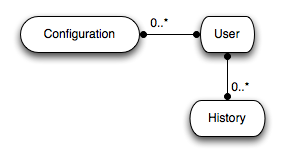
\includegraphics[scale=0.7]{user_model.png}
  \caption{User tables.}
  \label{fig:user_model}
\end{figure}

In the history table (Table \ref{tbl:history_table} on page \pageref{tbl:history_table}) each history row is referenced
in some other database table in order to store which user and when that table object
was created and who and when made the last modification/update.

\subsection{Taxonomy hierarchy}

The taxonomy objects presented in Section 3.3 are represented in the relational model as shown in Figure~\ref{fig:tax_model}.
Each tree is stored in the TaxonomyTree table (Table \ref{tbl:taxonomy_tree_table} on page \pageref{tbl:taxonomy_tree_table})
and can be referenced by
taxonomies themselves in the Taxonomy table (Table \ref{tbl:taxonomy_table} on page \pageref{tbl:taxonomy_table}). Each taxonomy can point to
a parent taxonomy and have multiple names represented in table
TaxonomyName (Table \ref{tbl:taxonomy_name_table} on page \pageref{tbl:taxonomy_name_table}).

In order to import taxonomies from external databases we created additional fields in the
Taxonomy table, which, at cost of space, gives us faster import times.
Each taxonomy name points to a TaxonomyNameType row (Table \ref{tbl:taxonomy_name_type_table} on page \pageref{tbl:taxonomy_name_type_table}),
which conveys the type of name we are trying to represent: synonyms, misspellings or something else.
Each taxonomy rank is stored at the TaxonomyRank table (Table \ref{tbl:taxonomy_rank_table} on page \pageref{tbl:taxonomy_rank_table}) and the rank itself can reference another parent rank.

\begin{figure}[H]
  \centering
    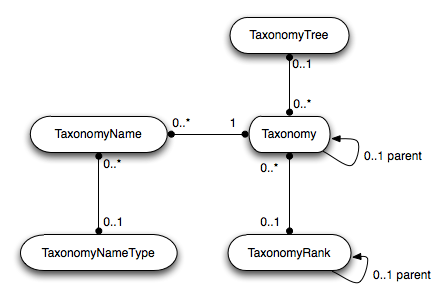
\includegraphics[scale=0.65]{tax_model.png}
  \caption{Taxonomies in the relational model}
  \label{fig:tax_model}
\end{figure}

\subsection{Sequence, labels and label instances}

The relational design to store sequences and sequence's annotations is one of the
most crucial and important aspect of the whole system,
as it will greatly affect the search performance and how the sequence annotation
will work at the storage level.

First, we designed a Sequence table (Table \ref{tbl:sequence_table} on page \pageref{tbl:sequence_table})
which stores all system sequences.
This table contains the value of the sequence's properties: name and content.
From the user perspective these two sequence properties
work as any other label, although they will skip the whole storage
mechanism described below and be stored right at the Sequence table.

\begin{figure}[H]
  \centering
    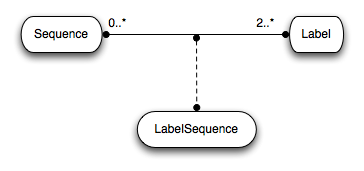
\includegraphics[scale=0.7]{labelseq_model.png}
  \caption{Label, sequences and label instances.}
  \label{fig:labelseq_model}
\end{figure}

To store label information which can be used to instantiate label instances
resulting in sequence annotations, we created the Label table (Table \ref{tbl:label_table} on page \pageref{tbl:label_table}).
For each Label row we store all the label properties (see Section \ref{sec:object_label}), type, metadata and code used
to be run at specific times in the system: automatic annotations, sequence modifications,
label values validation, etc.

With these two tables in place, we created another table,
LabelSequence (Table \ref{tbl:label_sequence_table} on page \pageref{tbl:label_sequence_table}),
which stores label instances, connecting a sequence with a label.

Each LabelSequence row contains fields for all kinds of data: integer, text, url, object, etc. But only one of these fields will be used to store the label value, if the label type is integer, only the integer data field will be used and everything else will be marked NULL.

One can argue that maintaining all those NULL fields are a waste of storage space.
Fortunately in MySQL's InnoDB storage engine NULL fields don't waste
unnecessary storage space, keeping the space costs at a minimum.
Other relational systems also employ similar optimizations. PostgreSQL for example,
uses bitmaps for NULL fields, only storing one bit for each NULL field and Oracle
uses a technique called 'trailing nulls', that optimizes table space when the NULL fields
appear at the row's end.

The Table \ref{tbl:label_types_fields} shows how each label type is stored in the LabelSequence table.

\begin{table}[H]
  \begin{tabular}{ | c | p{12cm} |}
    \hline
    \textbf{Type} & \textbf{Information} \\ \hline
    
    Integer & Stored in the \textit{int\_data} field. \\ \hline
    Text & \textit{text\_data}. \\ \hline
    Float & \textit{float\_data}. \\ \hline
    Bool & \textit{bool\_data}. \\ \hline
    Date & \textit{date\_data}. \\ \hline
    Url & \textit{url\_data}. \\ \hline
    Ref & References to other sequences are stored in the field \textit{ref\_data}. This field is a foreign key to the Sequence table. \\ \hline
    Obj & Reference to a file in the file table (field \textit{obj\_data}). \\ \hline
    Position & The starting position is stored in the field \textit{position\_start} and the length in \textit{position\_length}. \\ \hline
    Tax & References to taxonomies are stored in the column \textit{taxonomy\_data}. This field is a foreign key to the Taxonomy table. \\
    \hline
  \end{tabular}
  \caption{Label types and related fields.}
  \label{tbl:label_types_fields}
\end{table}

\subsection{Miscellaneous tables}

There are also other auxiliary tables that support non-core related tasks. For instance,
the event table (Table \ref{tbl:event_table}) stores the currently running events. Two kinds of events are supported:
add/edit of label instances in multiple labels, sequence importation. Each event row
contains information about some potentially long event in which the progress must be shown
in the user information. Each client polls event information using the event code to refresh
the interface.

Another auxiliary, yet important, table, is the file table (Table \ref{tbl:file_table}). The file table stores label instance information for object type labels. Each row stores the file and an integer, representing the number of label instances linking to this file. When a new label instance refers to this file the reference count is increment and when an instance is deleted the count is decremented. When reaching zero the file is released from the database.

\section{File formats} \label{sec:file_formats}


We use files to import or export data in order to interchange information between different kinds of systems or among various instances of the application. These files can be in two different kinds of formats: XML or FASTA.

Among other things, those files are used throughout the system to: copy entire databases, import sequences, install new labels, import whole taxonomy trees or heterogenous integration. 
 
\subsection{FASTA}

The FASTA format \cite{fasta} is very well known in the bioinformatics field as it is used to store a specific set of DNA or protein sequences.

In our system, this format is used to export stored sequences or to import new ones.

We have designed two FASTA-like formats:

\begin{itemize}
  \item Plain format
  
  In the plain format we just store the sequence name followed by its content.
  
\begin{lstlisting}[float, language=bash,frame=single,caption={Plain FASTA format.}]
>AK315637
ELRLRYCAPAGFALLKCNDADYDGFKTNCSNVSVVHCTNLMNTTVTTGLLLNGSYSENRT
QIWQKHRTSNDSALILLNKHYNLTVTCKRPGNKTVLPVTIMAGLVFHSQKYNLRLRQAWC
HFPSNWKGAWKEVKEEIVNLPKERYRGTNDPKRIFFQRQWGDPETANLWFNCHGEFFYCK
MDWFLNYLNNLTVDADHNECKNTSGTKSGNKRAPGPCVQRTYVACHIRSVIIWLETISKK
TYAPPREGHLECTSTVTGMTVELNYIPKNRTNVTLSPQIESIWAAELDRYKLVEITPIGF
APTEVRRYTGGHERQKRVPFVXXXXXXXXXXXXXXXXXXXXXXVQSQHLLAGILQQQKNL
LAAVEAQQQMLKLTIWGVK
<...more sequences...>
\end{lstlisting}
  
  \item Complex format
  
  In this format we also store label instance information along the sequence data. \\
  
  The format starts by including one line comment, followed by a line telling which labels are included for each sequence. Those labels are separated by the character '$|$'. If some label values are to be ignored, the label
  name should be skipped by placing an empty string followed by a '$|$'. \\
  
  For each sequence line we put all the label instances separated by the character '$|$'. The order of the label instances must be equal to the label's order at the file's header.\\
  
  If the sequence does not have a specific label instance the string in that column should be empty "".\\
  
  If the label instance value is empty and that label is not editable and can be generated from code it will be automatically generated when imported.
  
  For multiple labels, the label value is enclosed by square brackets '[]' and each instance, represented as \textit{param -$>$ value}, is separated by the character '§'.\\
  
  The special label 'name' is treated like any other label. If it is not included in the label's header, the
  first 10 sequence's content characters will be used by omission.
  
  An example of this format can be seen in Listing~\ref{ComplexFastaFormat}.\\
  
\begin{lstlisting}[float, language=bash,frame=single,breaklines=true,caption={Complex FASTA format example.}, label=ComplexFastaFormat]
;flavio - Monday 19th October 2009 07:06:33 PM - sequence id 465
#name|length|internal_id|perm_public|type|translated|url
>AK315637|1554|465|0|dna|AK315637_p|[google -> http://google.pt § ncbi -> http://www.ncbi.nlm.nih.gov/]
ELRLRYCAPAGFALLKCNDADYDGFKTNCSNVSVVHCTNLMNTTVTTGLLLNGSYSENRT
QIWQKHRTSNDSALILLNKHYNLTVTCKRPGNKTVLPVTIMAGLVFHSQKYNLRLRQAWC
HFPSNWKGAWKEVKEEIVNLPKERYRGTNDPKRIFFQRQWGDPETANLWFNCHGEFFYCK
MDWFLNYLNNLTVDADHNECKNTSGTKSGNKRAPGPCVQRTYVACHIRSVIIWLETISKK
TYAPPREGHLECTSTVTGMTVELNYIPKNRTNVTLSPQIESIWAAELDRYKLVEITPIGF
APTEVRRYTGGHERQKRVPFVXXXXXXXXXXXXXXXXXXXXXXVQSQHLLAGILQQQKNL
LAAVEAQQQMLKLTIWGVK (...)
<...more sequences...>
\end{lstlisting}
  
\end{itemize}

\subsection{XML}

The XML format is widely used to export and import lots of different kinds of data throughout the system. This format can handle labels, sequences, taxonomy trees, ranks and the database itself.

\begin{itemize}
  \item \textbf{Labels}
  
  Using the XML format we can export a set of labels. This file can then be imported in another system resulting in label installation or update. \\
  
  An example of this kind of file is shown in Listing~\ref{LabelXmlFile} and as it can be seen, we store each label property as a XML tag.
  
  All the rules concerning empty label instances from the complex FASTA format are also present in this format.
  
\begin{lstlisting}[float, language=xml, frame=single, label=LabelXmlFile, caption={An example Label XML file.}]
<labels>
  <label>
		<name>length</name>
		<type>integer</type>
		<comment></comment>
		<default>1</default>
		<must_exist>1</must_exist>
		<auto_on_creation>1</auto_on_creation>
		<auto_on_modification>1</auto_on_modification>
		<code>return strlen($content);</code>
		<valid_code>return $data &gt; 0;</valid_code>
		<editable>0</editable>
		<deletable>0</deletable>
		<multiple>0</multiple>
		<public>1</public>
	</label>
	<...more labels...>
</labels>
\end{lstlisting}

\item \textbf{Sequences}

Besides the FASTA format, sequences can also be stored in XML files. The main difference between the FASTA format is that, given the structured and flexible nature of XML, it is easier to describe the sequence contents and its label instances.

\begin{lstlisting}[float, language=xml, frame=single, label=SequenceXmlFile, caption={An Sequence XML file.}]
<sequences>
<author>flavio</author>
<date>Tuesday 20th October 2009 12:59:53 AM</date>
<what>sequence id 465</what>
<labels>
	<label>length</label>
	<label>internal_id</label>
	<label>perm_public</label>
	<label>type</label>
	<label>translated</label>
	<label>url</label>
</labels>
<sequence>
	<name>AK315637</name>
	<content>ELRLRYCAPAGFALLKCNDADYDGFKTNCSNVSVVHCTNLMNTTVTTGLLLNGSYSENRT
  QIWQKHRTSNDSALILLNKHYNLTVTCKRPGNKTVLPVTIMAGLVFHSQKYNLRLRQAWC
  HFPSNWKGAWKEVKEEIVNLPKERYRGTNDPKRIFFQRQWGDPETANLWFNCHGEFFYCK
  MDWFLNYLNNLTVDADHNECKNTSGTKSGNKRAPGPCVQRTYVACHIRSVIIWLETISKK
  TYAPPREGHLECTSTVTGMTVELNYIPKNRTNVTLSPQIESIWAAELDRYKLVEITPIGF
  APTEVRRYTGGHERQKRVPFVXXXXXXXXXXXXXXXXXXXXXXVQSQHLLAGILQQQKNL
  LAAVEAQQQMLKLTIWGVK (...)</content>
	<label name="length">1554</label>
	<label name="internal_id">465</label>
	<label name="perm_public">0</label>
	<label name="type">dna</label>
	<label name="translated">AK315637_p</label>
	<label name="url" param="google">http://google.pt</label>
	<label name="url" param="ncbi">http://www.ncbi.nlm.nih.gov/</label>
</sequence>
</sequences>
\end{lstlisting}

The same sequence represented in FASTA (Listing~\ref{ComplexFastaFormat}) can be seen formatted as XML in Listing~\ref{SequenceXmlFile}.
  
  \item \textbf{Ranks}
  
  To manage ranks across multiple application instances we designed a XML format to store taxonomy ranks.
  
\begin{lstlisting}[float, language=xml, frame=single, label=RankXmlFile, caption={An example Rank XML file.}]
<ranks>
	<rank>
		<name>class</name>
		<parent>phylum</parent>
	</rank>
	<rank>
		<name>family</name>
		<parent>order</parent>
	</rank>
	<...more ranks...>
</ranks>
\end{lstlisting}
  
  As it can be seen in Listing~\ref{RankXmlFile}, for each rank we register its name and parent rank. This type of files is useful to copy rank sets around systems.
  
  \item \textbf{Taxonomy trees}
  
  We designed a XML format to store taxonomy trees, which is very useful to easily copy an entire taxonomy tree from one system to another.
  
\begin{lstlisting}[float, language=xml, frame=single, label=TaxonomyTreeXmlFile, caption={An example Taxonomy tree XML file.}]
<tree>
	<name>example</name>
	<nodes>
		<taxonomy>
			<name>root_taxonomy</name>
			<rank>family</rank>
			<taxonomy>
				<name>child_taxonomy</name>
				<rank>genus</rank>
			</taxonomy>
			<taxonomy>
				<name>child_taxonomy2</name>
				<rank>genus</rank>
			</taxonomy>
		</taxonomy>
	</nodes>
</tree>
\end{lstlisting}
  
  In this format, we store the tree name followed by a 'nodes' tag which will store, starting by the root taxonomies, the taxonomies from this tree. Each 'taxonomy' tag may contain an arbitrary number of 'taxonomy' tags which represent taxonomy's children.
  
  \item \textbf{Database}
  
  We designed another XML based format, this time to store the entire database. The skeleton for this format is presented in Listing~\ref{DatabaseXmlFile} and it is organized as follows:
  
  \begin{itemize}
    \item \textbf{labels}
    
    This section is exactly the same as the Label XML file.
    
    \item \textbf{ranks}
    
    Idem, but for ranks.
    
    \item \textbf{trees}
    
    A special tag containing all the taxonomy trees. Each tree is represented the way it is shown for the Taxonomy tree XML file.
    
    \item \textbf{sequences}
    
    This section follows the Sequence XML file structure.
    
  \end{itemize}

  \begin{lstlisting}[float, language=xml, frame=single, label=DatabaseXmlFile, caption={Database in XML skeleton.}]
  <biodata>
    <...labels...>
    <...ranks...>
    <trees>
      <...all taxonomy trees...>
    </trees>
    <...sequences...>
  </biodata>
  \end{lstlisting}

\end{itemize}

\subsection{CSV}

The CSV format is used to display distribution values over a set
of sequences and a numeric label. Once copied, this information can be used in spreadsheet programs.

Another use of the CSV format is to export a sequence list and a selected set of labels.
The file header contains the list of labels that are represented and each line contains a single
sequence. Multiple label values are separated by the character \texttt{;} and each value is of
the form \texttt{paramater : value}.

An example CSV file is shown in Listing \ref{SequencesCSV}.

\begin{lstlisting}[float, language=bash, frame=single, label=SequencesCSV, caption={An example CSV file.}]
name , length , type
seq1 , 513 , dna
seq2 , 231 , protein
seq3 , 85 , dna
\end{lstlisting}

\section{Query language}\label{sec:grammar}

A simple, yet arbitrarily complex, query language was designed to search
stored sequences using annotated information present in label instances.

A simplified grammar in BNF format for this language is shown in Figure \ref{fig:query_bnf}.
Note that every label supports two basic unary operators: \textbf{exists} and \textbf{notexists}, when
used they filter sequences that contain any value label or no value at all, respectively.
Queries can be nested using the AND, OR and NOT operators. Parenthesis can also be used to group expressions.

\begin{figure}[ht]
\begin{grammar} 
[(colon){$\rightarrow$}] 
[(semicolon)$|$] 
[(comma){}] 
[(period){\\}] 
[(quote){\begin{bf}}{\end{bf}}] 
[(nonterminal){$\langle$}{$\rangle$}]
<expression>:<expression> AND <expression>; <expression> OR <expression>; NOT <expression>;(<expression>) ; <terminal>.
<terminal>:<label name>,<unary operators>;<bool terminal>;<integer terminal>;<float terminal>;<position terminal>;<taxonomy terminal>;<text terminal>;<url terminal>; <obj terminal>; <date terminal>.
<bool terminal>:<label name>;<label name>,<bool operators>,<bool value>.
<bool operators>:<base operators>.
<bool value>: "true"; "false".
<unary operators>:"exists";"notexists".
<base operators>:"is"; "$=$"; "eq"; "equal".
<integer terminal>:<label name>,<numeric operators>,<integer value>.
<float terminal>:<label name>,<numeric operators>,<float value>.
<position terminal>:<label name>,<position type>,<numeric operators>,<integer value>.
<numeric operators>:<base operators>;"$\greaterthan$"; "$\greaterthan=$"; "$\lessthan$"; "$\lessthan=$".
<position type>:"start";"length".
<taxonomy terminal>:<label name>,<taxonomy operators>,<label value>.
<taxonomy operators>:<base operators>; "like".
<url terminal>:<label name>,<text operators>,<url>.
<text terminal>:<label name>,<text operators>,<label value>.
<text operators>:<base operators>;"contains"; "starts"; "ends"; "regexp".
<obj terminal>:<text terminal>.
<date terminal>:<label name>,<date operators>,<date value>.
<date operators>:<base operators>; "after"; "before".
<date value>:<day>,"-", <month>, "-", <year>.
<label name>: <base label name>;<base label name>, "[", <string>, "]".
<base label name>:"{\tt\quotesymbol}",<string>,"{\tt\quotesymbol}"; <string>.
<label value>:"{\tt\quotesymbol}",<string>,"{\tt\quotesymbol}"; <string>.
\end{grammar}
\caption{Query language written in BNF.}
\label{fig:query_bnf}
\end{figure}

All labels support a basic set of operators: \textbf{is}, \textbf{=}, \textbf{eq} and \textbf{equal}. All those operators do the same thing and, depending on the label type, they filter sequences which contain the specified label value.

We can also specify a multiple label instance with the parameter selector, using \textit{label\_name{[parameter]}}. If an expression involves a multiple label that is not parameter specific, all label instances will be considered, instead of only one.

The following list specifies the differences for each label type:

\begin{itemize}
  \item \textbf{Bool}
  
  Labels of this type can use the equal operation on values \textit{true} or \textit{false}. We can also skip the operator and value altogether and only keep the label name, as the example: \textit{dna and length $>$ 5} instead of \textit{dna is true and length $>$ 5}. 
  
  \item \textbf{Integer and float}
  
  Numeric labels use the basic comparison operators: \textbf{=}, \textbf{$>$}, \textbf{$>=$}, \textbf{$<$}, \textbf{$<=$}.

  \item \textbf{Position}
  
  For position labels we must first select between the start or the length component, and then an integer operator.
  Example: \textit{label\_name start $>$ 5}.
  
  \item \textbf{Taxonomy and reference}
  
  For these kinds of labels we can also use the operator \textbf{like}, which has the same effect as the standard equal operator. Those operators work by searching all sequences or taxonomies where the name matches the provided regular expression and then filtering the result list of sequences who have at least one label instance point to the same sequence or taxonomy of the former search result.
  
  \item \textbf{Url and text}
  
  For these label types the operators provided are: \textbf{starts} (if the string starts with the provided value),
  \textbf{ends} and \textbf{regexp}, for regular expression matches.
  
  \item \textbf{Object}
  
  Object labels can use the same text operators to search the filename associated with the label instance.
  
  \item \textbf{Date}
  
  Date labels provide day based operators: \textbf{equal} (in the same day), \textbf{after} (after the day),
  \textbf{before} (before the day).
\end{itemize}

\clearpage
\chapter{Implementation}

This section describes certain implementation aspects worthy to be mentioned and so, are particularly important to better understand the system.

We will cover technological aspects related to the application's architecture, database optimizations and how queries work and are translated into raw SQL code. Other important particularities like automatic label instantiation and code storage will also be analyzed.

Some aspects that we barely or not mentioned at all in the Design section will be presented in more depth here.

\section{Technology}

Given the program description made on chapter \ref{sec:introduction}, its base architecture
and restrictions, we had to chose a set of technologies to use in the implementation.
Being a web application, we will differentiate between server and client technologies.

\subsubsection{Server side}

\begin{itemize}
  \item \textbf{Apache}
  
  Apache \cite{apache} is used as the application's web server. It is a very widely used web server across the Internet.
  
  \item \textbf{MySQL}
  
  The relational database system used to store application data. MySQL \cite{mysql} is open source software.
  
  \item \textbf{PHP and CodeIgniter}
  
  PHP \cite{php} is a very widely used programming language to implement dynamic websites. \textit{CodeIgniter} \cite{codeigniter} is a full-featured PHP web-development framework, it adheres to the Model View Controller (MVC) design pattern to build web applications.
  
  \item \textbf{Smarty}
  
  Smarty \cite{smarty} was used for the View component of the MVC pattern of \textit{CodeIgniter}, functioning as an html template engine.
  
  \item \textbf{EMBOSS}
  
  EMBOSS \cite{emboss} offers a very complete set of bioinformatics programs. It is used to compute the values for certain labels.
  
  \item \textbf{Python and MySQLdb}
  
  Python \cite{python} is a dynamic scripting language and it was used to run small database scripts to install and update default system data. In the process, we used the MySQLdb \cite{mysqldb} plugin for database interfacing.
  
\end{itemize}

\subsubsection{Client side}

On the client side we used the standard HTML, CSS, JavaScript, and jQuery.
Several jQuery plugins are used to easily implement certain types
of user interface components.

\begin{itemize}
  \item \textbf{HTML}
  
  HyperText Markup Language is the predominant markup language for web pages.
  
  \item \textbf{CSS}
  
  CSS is a style sheet language used to describe the look and formating of a document written in HTML.
  
  \item \textbf{JavaScript}
  
  Object oriented language available in the browser and used to dynamically change the web page content.
  
  \item \textbf{jQuery}
  
  jQuery is a client side javascript framework that concentrates on the "write less do more philosophy", it abstracts away browser incompatibilities and offers an easy way to manipulate DOM objects and write client logic.
  
  Techniques like asynchronous Javascript and XML are supported by jQuery. The library also supports plugins make it a flexible and open architecture.
  
  \item Impromptu - \url{http://trentrichardson.com/Impromptu/index.php}
  
  Impromptu is an extention to help provide a more pleasant way to spontaneously prompt a user for input. More or less this is a replacement for an alert, prompt, and confirm.
  
  \item Autocomplete - \url{http://bassistance.de/jquery-plugins/jquery-plugin-autocomplete/}
  
  Used to autocomplete an input field to enable users to quickly find and select some value, leveraging searching and filtering. The plugin can use remote sources, through AJAX.
  
  \item blockUI - \url{http://malsup.com/jquery/block/}
  
  BlockUI can block the user interface, simulating synchronous behavior when using AJAX. Widely used
  for \textit{loading} screens.
  
  \item jQuery confirm - \url{http://nadiana.com/jquery-confirm-plugin}
  
  It displays a confirmation message before doing any image. Used to confirm data deletion.
  
  \item jeditable - \url{http://www.appelsiini.net/projects/jeditable}
  
  This plugin can transform a block of text into an input component, send the new data to the server and
  redisplay the original data. Used to in-place edit of fields.
  
  \item ThickBox - \url{http://jquery.com/demo/thickbox/}
  
  Its function is to show a single image, multiple images, inline content, iframed content, or content served through AJAX in a hybrid modal.
  
  \item jQuery validate - \url{http://bassistance.de/jquery-plugins/jquery-plugin-validation/}
  
  This plugin features an automatic form validation per field, displaying error messages when the user tries
  to send the form.
  
  \item TextGrow - \url{http://remysharp.com/2006/11/27/delicious-like-text-grow-jquery-plugin-2/}
  
  TextGrow when applied to a text field enables the field to grow as the user types text in it.
  
  \item jQuery UI - \url{http://jqueryui.com/}
  
  We used the date picker widget and some effects.
    
\end{itemize}

\section{Authentication}

In the system we have two kinds of users:

\begin{itemize}
  \item \textbf{Normal user}
  
  Can do pretty much anything, except disable users, install new labels and do database management.
  
  \item \textbf{Administrator}
  
  Can do everything the normal user can do and: list users, disable users, install labels, cleanup the database,
  import database data, and change the database description.
\end{itemize}

The user type is stored along the user data.

Each user has a password to access the system. For each password we create a salted MD5 hash and then store it in the specific user row. To check if the password provided by the user is valid we generate a salted MD5 hash of the input and compare it to the stored hash.

This mechanism is widely used to prevent user passwords from being stolen when the database is compromised.

When the user successfully logs in we use the Session abstraction provided by \textit{CodeIgniter} to indicate that the user is logged in for the next HTTP transactions. 

\section{Recording modifications}

When a specific system object is modified or created, we need to store the user and time of that modification or creation, respectively.
This information is used in the following tables: \textit{user}, \textit{label}, \textit{label\_sequence}, \textit{sequence}, \textit{taxonomy}, \textit{taxonomy\_rank} and \textit{taxonomy\_tree}. Each table has an history\_id field which points to an history's table record. Each record stores pointers to creation and update users and respective time stamps.

We created triggers that automatically delete history information when any database record using it is removed.
Update and insert triggers were also put in place to automatically update time information. As the system
can generate an enormous amount of label instances, no insert trigger exists for the \textit{label\_sequence} table,
and it is only when a row is modified that a new history record is created.

Some abstractions were created to automatically insert or update new database information along with history data.
These abstractions are implemented in the \textit{BioModel} class.

The BioModel class also implements some frequently used database operations and is used to subclass nearly all database models.

To know if the user is and who is logged in, we use the Session's data mentioned in the previous sub-section.

\section{Tables and views}

Apart from using the tables mentioned in the Relational Model Design's section, we also created tables views. These table views are used across the application to shorten SQL queries.

The views created, for each table, are the following:

\begin{itemize}
  \item \textbf{history}
  
  \begin{itemize}
    \item history\_info - Joins the history table with the user table, to retrieve user information of the last update or creation.
  \end{itemize}
  
  \item \textbf{label}
  
  \begin{itemize}
    \item label\_norm - Altered label table with the id column changed to label\_id. Used by other views.
    \item label\_info\_history - View joining label\_norm and history\_info views.
  \end{itemize}
  
  \item \textbf{label\_sequence}
  
  \begin{itemize}
    \item label\_sequence\_extra - The table label\_sequence joined with the taxonomy, sequence and file tables. The purpose is to display the taxonomy name and sequence name for label instances of the label types taxonomy and reference, respectively.
    \item label\_sequence\_info - label\_sequence\_extra joined with label\_norm.
  \end{itemize}
  
  \item \textbf{sequence}
  
  \begin{itemize}
    \item sequence\_info\_history - Table sequence joined with history\_info view.
  \end{itemize}
  
  \item \textbf{taxonomy}
  
  \begin{itemize}
    \item taxonomy\_info - Taxonomy table joined with taxonomy\_rank and taxonomy\_tree, making access to taxonomy rank and tree name easy.
    \item taxonomy\_info\_history - taxonomy\_info joined with history\_info.
  \end{itemize}
  
  \item \textbf{taxonomy\_name}
  
  \begin{itemize}
    \item taxonomy\_name\_info - taxonomy\_name table joined with taxonomy\_name\_type.
  \end{itemize}
  
  \item \textbf{taxonomy\_name\_type}
  
  \begin{itemize}
    \item taxonomy\_name\_type\_norm - taxonomy\_name\_type table normalized to use in taxonomy\_name\_info view.
  \end{itemize}
  
  \item \textbf{taxonomy\_rank}
  
  \begin{itemize}
    \item taxonomy\_rank\_norm - taxonomy\_rank table normalized to use in other views.
    \item taxonomy\_rank\_parent\_norm - taxonomy\_rank table normalized to use in taxonomy\_rank\_info.
    \item taxonomy\_rank\_info - Uses taxonomy\_rank\_norm and taxonomy\_rank\_parent to display the rank and parent rank name.
    \item taxonomy\_rank\_info\_history - taxonomy\_rank\_info joined with history\_info.
  \end{itemize}
  
  \item \textbf{taxonomy\_tree}
  
  \begin{itemize}
    \item taxonomy\_tree\_norm - taxonomy\_tree normalized.
    \item taxonomy\_tree\_info\_history - taxonomy\_tree\_norm joined with history\_info. 
  \end{itemize}
  
  \item \textbf{user}
  
  \begin{itemize}
    \item user\_norm - User table normalized to use in other views.
    \item user\_norm\_creation - View used to create history\_info.
  \end{itemize}
\end{itemize}

The transactional storage engine used for the tables is InnoDB \cite{innodb}. The main advantages of this storage engine are: \textit{row-level locking}, \textit{ACID compliant transactions}, \textit{foreign key constraints support} and crash recovery. The support of foreign key constraints and ACID transactions were the biggest advantages against other engines like MyISAM.

\section{Database optimizations}

To shorten query execution time and disk space used, various database optimizations were made.

\subsubsection{Space optimizations}

For space related optimizations, we tried to carefully choose each column data type paying attention for how much space we needed for each piece of data. Appendix \ref{app:tables} describes data types for each table. 

\subsubsection{Query time optimizations}

Some table fields are more crucial to search performance than others. With this in mind,
we enumerated the most important fields and then created appropriate indexes for them.

In the following list we present the indexes created for each table:

\begin{itemize}
  \item \textbf{user}
  
  \begin{itemize}
    \item id - to locate user's using the id.
    \item name - name is 32 bytes string and the index has the same size. Used to locate users by name.
    \item history\_id - foreign key index.
  \end{itemize}
  
  \item \textbf{configuration}
  
  \begin{itemize}
    \item user\_id, key - used to search configuration values using the user id and configuration key.
    \item user\_id - foreign key index.
  \end{itemize}
  
  \item \textbf{event}
  
  \begin{itemize}
    \item id - primary key index.
    \item event\_code - to locate events using the event code.
  \end{itemize}
  
  \item \textbf{file}
  
  \begin{itemize}
    \item id - primary key index.
    \item label\_id, name - unique index.
    \item label\_id - foreign key index.
  \end{itemize}
  
  \item \textbf{history}
  
  \begin{itemize}
    \item id - to locate history records using the id / primary key index.
    \item creation\_user\_id - foreign key index to creation user.
    \item update\_user\_id - foreign key index to update user.
  \end{itemize}
  
  \item \textbf{label}
  
  \begin{itemize}
    \item id - primary index.
    \item name - unique index and to locate labels by name.
    \item history\_id - foreign key index.
    \item label\_type - to locate labels by type.
  \end{itemize}
  
  \item \textbf{label\_sequence}
  
  \begin{itemize}
    \item id - primary index.
    \item history\_id - foreign key index.
    \item label\_id - foreign key index. To search label instances by label.
    \item seq\_id - foreign key index. To search label instances by sequence.
    \item seq\_label\_id - for faster searches using sequence and label id.
    \item ref\_data - foreign key index. To locate the sequence this reference label points to.
    \item tax\_data - foreign key index. To locate the taxonomy this taxonomy label points to.
    \item obj\_data - foreign key index. To locate the file this object label points to.
    \item int\_data - for faster searches of integer label values.
    \item float\_data - for faster searches of float label values.
    \item text\_data - index with size 16 to locate text labels.
  
  \end{itemize}
  
  \item \textbf{sequence}
  
  \begin{itemize}
    \item id - primary index.
    \item history\_id - foreign key index.
    \item content - index with size 16 to do faster sequence searches using content.
    \item name - index with size 16 to locate sequences by name.
  \end{itemize}
  
  \item \textbf{taxonomy}
  
  \begin{itemize}
    \item id - primary index.
    \item import\_id - to locate taxonomies using the import id.
    \item rank\_id - foreign key index. To locate taxonomies using rank.
    \item history\_id - foreign key index.
    \item tree\_id - foreign key index. To locate taxonomies by tree.
    \item parent\_id - foreign key index. To locate taxonomies by parent.
    \item import\_parent\_id - to locate taxonomies using the parent import id.
    \item name - index with size 16 to locate taxonomies by name.
  \end{itemize}
  
  \item \textbf{taxonomy\_name}
  
  \begin{itemize}
    \item id - primary index.
    \item type\_id - foreign key index. To locate names by type.
    \item tax\_id - foreign key index. To locate specific taxonomy's names.
  \end{itemize}
  
  \item \textbf{taxonomy\_name\_type}
  
  \begin{itemize}
    \item id - primary index.
    \item name - index with size 5 to locate name types by name.
  \end{itemize}
  
  \item \textbf{taxonomy\_rank}
  
  \begin{itemize}
    \item id - primary index.
    \item name - unique index.
    \item history\_id - foreign key index.
    \item parent\_id - foreign key index. To locate ranks by parent.
  \end{itemize}
  
  \item \textbf{taxonomy\_tree}
  
  \begin{itemize}
    \item id - primary index.
    \item name - unique index. To locate trees by name.
    \item history\_id - foreign key index.
  \end{itemize}
\end{itemize} 

\section{Label generation}

Our system supports automatic label generation using stored code to generate label instances in the database.

All the code stored is written in PHP and is evaluated with sequence and label
information loaded in the execution environment (Table \ref{tbl:label_generation_env}).
All those variables can be used to generate a new label instance.

\begin{table}[H]
  \begin{tabular}{ | >{\centering}m{20mm} | p{12cm} |}
    \hline
    \textbf{Name} & \textbf{Description} \\ \hline
    sequence & array containing sequence information: id, name, content, creation and update status. \\ \hline
    id & sequence id. \\ \hline
    name & sequence name. \\ \hline
    content & sequence content. \\ \hline
    label\_id & generating label id. \\ \hline
    label\_name & generating label name. \\ \hline
    this & pointer to the model instance and \textit{CodeIgniter} libraries. \\ \hline
  \end{tabular}
  \caption{Label generation environment.}
  \label{tbl:label_generation_env}
\end{table}

When generating a multiple label value the code should return an array of \textbf{LabelData} instances.
\textbf{LabelData} groups a multiple label parameter and a label value.

\subsubsection{Auto-creation labels}

The field \textit{auto\_creation} on the \textbf{label} table is used to generate a label instance for
a newly created instance.
If this field is TRUE the code stored in the \textbf{code} field is run against the environment presented before
to generate a new label instance. If the value returned by the code is \textbf{null} or an
exception is thrown, the new label instance is not added.

When inserting a new sequence into the system we fetch all labels with \textit{auto\_creation}
set to \textbf{TRUE} and then we run the process for each label found.

\subsubsection{Auto-modification labels}

When changing the sequence content the system can, based on the sequence's label instances, select
those labels in which property \textit{auto\_modification} is set to \textbf{TRUE} and
then regenerate the instance values.

For each label instance we run the code stored in the \textbf{code} field to generate the new values.
If the label has multiple values and is not editable then we remove all the previous label instances.

\subsubsection{Action-modification labels}\label{sec:action_modification}

Another helpful feature in generating label instances is action-modification labels. Those labels
have the field \textbf{action\_modification} filled with PHP code, and can be executed to perform
some maintenance function when the sequence content is altered.

For example, we could remove label instances of a label type when the content is changed in some arbitrary way.

\subsubsection{Validating label instances}

When inserting or updating label values the system supports custom validation through the \textbf{valid\_code}
\textbf{label} field. This field can contain arbitrary code that should return \textbf{TRUE} or \textbf{FALSE}
when the value is valid or not, respectively. It is useful to validate user input and limit label values.

When executing the validation code, apart from the environment values shown before, we also make the label
value available as the \textbf{data} variable.

If the data value is a multiple label instance, the user should use the functions \textbf{label\_get\_data} and
\textbf{label\_get\_param} to get the real label value and the label parameter, respectively.

\section{Search}

The search functionality is handled by the \textit{Search controller} and the \textit{Search model}.
The \textit{Search model} handles SQL query generation and the controller provides
an JSON/AJAX based interface to communicate with clients.

The http method \textbf{search/get\_search} can receive as POST arguments
the following list:

\begin{itemize}
  \item \textbf{start}: start of result list.
  \item \textbf{size}: size of returned result list.
  \item \textbf{search}: the serialized JSON object representing the query.
  \item \textbf{labels}: list of labels attached to the result list.
  \item \textbf{transform}: the label in which we will transform the results. We will talk about this later on.
  \item \textbf{disable\_ordering}: if this parameter contains something, the sequences will not be ordered by name.
\end{itemize}

For convenience, the http method \textbf{search/get\_search\_total} can return the
number of sequences for a specific query. When we know the total number of rows,
it is then possible to fetch partial results using the \textbf{get\_search} method.

\subsection{Query trees}

To represent query expressions our system uses a tree like structure.
The search term is represented as a JSON\cite{json} object. The query
is generated by the client and sent, in a serialized form, through
the network to the server, the object is then de-serialized and transformed
into an object that can be read using PHP.
The server uses the new object to generate the equivalent SQL
query expression and then fetch all results from the database.
These results are then sent back to the client.

A search/query expression can recursively be defined as:

\begin{itemize}
  \item \textbf{Terminal expression}
  
  Forms the basic expression, contains the target label, an operator and, optionally, the value to compare.
  \begin{lstlisting}[float, language=bash, frame=single, label=terminal_expression_json, caption={Terminal expression as a JSON object}]
  {label: "length", oper:"gt", value: "500"}
  \end{lstlisting}
  
  A terminal expression is shown in Listing \ref{terminal_expression_json} (meaning \textit{length $>$ 500}). The \textbf{label} property accepts the search label, the \textbf{oper} property is the operator
  and the value used in the expression is put in the \textbf{value} property. \\
  
  If the label is multiple, the expression can be extended with the \textbf{param} property,
  indicating the multiple parameter to use. Listing \ref{terminal_expression_json_param} displays the JSON object for the
  expression \textit{url[info] = "\url{http://mysite.com}"}.\\
  
  \begin{lstlisting}[float, language=bash, frame=single, label=terminal_expression_json_param, caption={Parametrized terminal expression}]
  {label: "url", param: "info", oper:"eq", value: "http://mysite.com"}
  \end{lstlisting}
  
  See Table \ref{tbl:search_operators_values_query} for a complete list of operators and values for each label type. \\
  
  \item \textbf{Structured expression}
  
  A structured expression groups other expressions (terminal or structured) using the special operators: AND, OR and NOT.
  AND and OR can have as arguments multiple expressions, the NOT operator can have only one expression: the expression to negate.
  \\ \\
  For the example shown in Listing \ref{structured_expression_json}
  $<$\textit{(length $>$ 500 and name exists) or content regexp AGTG}$>$ we can see
  that each structured expression contains
  the \textbf{oper} property naming the special operator and the \textbf{operands} property which contains a list
  of expressions.\\ \\
  
  \begin{lstlisting}[float, language=bash, frame=single, label=structured_expression_json, caption={Structured expression as a JSON object}]
  {oper: "or",
   operands: [
    { oper: "and",
      operands: [
        {label: "length", oper: "gt", value: "500"},
        {label: "name", oper: "exists"}
      ]
    },
    {label: "content", oper: "regexp", value:"AGTG"}
   ]
  }
  \end{lstlisting}
  
\end{itemize}

\begin{table}[ht]
  \scalebox{0.8}{%
    \begin{tabular}{ | c | p{0.4\textwidth} | p{0.55\textwidth} |}
      \hline
      \textbf{Label type} & \textbf{Operators} & \textbf{Values} \\ \hline
      
      URL, text and object & \begin{itemize}
        \item \textit{eq}: Equal comparison.
        \item \textit{contains}: If the label contains a substring.
        \item \textit{starts}: If the instance starts with.
        \item \textit{ends}: Starts counterpart.
        \item \textit{regexp}: Regular expression matching.
      \end{itemize} & The value should be a string for all operators. \\ \hline
      
      Bool & \begin{itemize}
        \item \textit{eq}: Equal comparison.
      \end{itemize} & The value should contain \textbf{true} or \textbf{false}. \\ \hline
      
      Integer and float & \begin{itemize}
        \item \textit{eq}: $=$
        \item \textit{gt}: $>$
        \item \textit{lt}: $<$
        \item \textit{ge}: $>=$
        \item \textit{le}: $<=$
      \end{itemize} & Values should be serialized numbers as strings. \\ \hline
      
      Position & \begin{itemize}
        \item \textit{eq}: $=$
        \item \textit{gt}: $>$
        \item \textit{lt}: $<$
        \item \textit{ge}: $>=$
        \item \textit{le}: $<=$
      \end{itemize} & Values should be an object with the property \textbf{num}
      containing the value and the \textbf{type} property with either \textit{start}
      or \textit{length}, to indicate the position component to compare. \\ \hline
      
      Date & \begin{itemize}
        \item \textit{eq}: Equal comparison.
        \item \textit{before}: Date is before some date.
        \item \textit{after}: Date is after some date.
      \end{itemize} & Values should be in the form \textit{dd-mm-yyyy} like \textit{03-11-2009} \\ \hline
      
      Taxonomy & \begin{itemize}
        \item \textit{eq}: Equal comparison.
        \item \textit{like}: A taxonomy name to search for.
      \end{itemize} & For the \textbf{eq} operator the value should be an object with the property \textbf{id}
      indicating the taxonomy ID. The \textbf{like} operator gets a taxonomy name and then searches all taxonomies
      with that name in the system and if the sequence points to any of them the query succeeds. \\ \hline
      
      Reference & \begin{itemize}
        \item \textit{eq}: Equal comparison.
        \item \textit{like}: A sequence name to search for.
      \end{itemize} & The values and operators work just like the taxonomy labels, but applied for sequences. \\ \hline
  \end{tabular}}
  \caption{Operators and values in query objects.}
  \label{tbl:search_operators_values_query}
\end{table}

For all label types the operators \textbf{exists} and \textbf{notexists} are also available.
These operators do not need the \textbf{value} property, but they can also use the multiple
label parameter to check the existence of a specific multiple label instance.

\subsubsection{Generating SQL from query trees}

Before retrieving the results from the database, the system needs to transform
a query object into an SQL expression, which MySQL can understand and execute.


\begin{algorithm}[ht]
  \SetLine
  \ForAll{Query Sub-Expressions}{
    Check for errors\;
    Get label information from the database if a new label reference appears\;
  }
  \BlankLine
  Expand query expression: \Begin{
    \ForAll{Query Sub-Expressions}{
      Expand the query object to simplify it\;
      Transform reference and taxonomy 'like' operator into an OR, searching before hand for sequences or taxonomies that match\;
    }
    expanded\_query\_object $\leftarrow$ generate new expanded query object\;
  }
  \BlankLine
  Transform \textit{expanded\_query\_object} into SQL:
  \Begin{
    \If{query is structured}{
      \If{special operator is NOT}{
        Grab the first argument\;
        sql\_transform $\leftarrow$ recursively transform argument into SQL\;
        \Return "NOT sql\_transform"\;
      }
      \ElseIf{special operator is AND or OR}{
        sql\_arguments $\leftarrow$ ""\;
        \ForAll{Arguments}{
          sql\_argument $\leftarrow$ recursively transform argument into SQL\;
          sql\_arguments $\leftarrow$ sql\_arguments + special operator + sql\_argument\;
        }
      }
    }
    \ElseIf{query is terminal}{
      \If{label is special}{
        \Return Special SQL code for each field\;
      }
      \ElseIf{label is standard}{
        oper $\leftarrow$ transform query operator into an SQL operator\;
        value $\leftarrow$ transform query value into an SQL value\;
        field $\leftarrow$ get table field for this label type\;
        \If{expression is multiple parameterized}{
          param\_sql $\leftarrow$ build SQL code for parameter\;
        }
        \Return "EXISTS(SELECT label\_sequence.id FROM label\_sequence WHERE label\_sequence.seq\_id = sequence.id AND label\_sequence.label\_id = " + label\_id + " AND " + field + " " + oper + " " + value + param\_sql + ")"\;
      }
    }
  }
  \caption{SQL search algorithm. \label{sql_search_algorithm}}
\end{algorithm}

Algorithm~\ref{sql_search_algorithm} builds an SQL WHERE expression to use in a number of
SQL queries: to fetch search total, to fetch sequences, to transform a result list, etc.

For example when searching for sequences where $<$\textit{(length $>$ 500 and name exists) or content regexp AGTG}$>$
the SQL to fetch the result is shown in Listing \ref{sql_example}.

\begin{lstlisting}[float, language=sql, frame=single, label=sql_example, caption={Resulting SQL query.}]
SELECT id, name
FROM sequence
WHERE ((EXISTS(SELECT label_sequence.id FROM label_sequence
               WHERE label_sequence.seq_id = sequence.id
          AND label_sequence.label_id = 1 AND int_data > 500 ))
      AND (TRUE)) OR (content REGEXP 'AGTG')
ORDER BY `name` ASC
\end{lstlisting}

\subsection{The transform label}

The query result can also be transformed by a specified label, that is, the user can input a label of type reference
to transform all the sequences into the corresponding reference label instance.

If the original results only contain DNA sequences and if all those sequences contain a label
named \textbf{protein} that links to the corresponding protein sequence, we can transform the results
to get all the related protein sequences.

The transform operation happens at SQL code generation time. The template generated for this is shown in
Listing \ref{sql_transform}, where \textbf{sql\_where} is the resulting SQL WHERE condition mentioned
before and \textbf{transform\_label} is the transform label ID.

\begin{lstlisting}[float, language=sql, frame=single, label=sql_transform, caption={Transform label SQL code template.}]
SELECT id, name
FROM  sequence
WHERE id IN (SELECT ref_data
             FROM label_sequence AS trans
             WHERE trans.label_id = $transform_label AND
                   trans.seq_id IN (SELECT id FROM sequence WHERE $sql_where) AND
                   ref_data IS NOT NULL)
ORDER BY 'name' ASC
\end{lstlisting}

\subsection{Parsing written queries}

The system features a search box where the user can write textual queries and get results.
For example, one can input $<$\textit{(length $>$ 500 and name exists) or content regexp AGTG}$>$
and the application will build the query JSON object to fetch the results.

Query parsing is performed in the server side and the client only sends the query text.
First, a \textit{tokenizer} class is used to separate the query text into tokens.
These tokens are then processed by the parser, which builds the query object.

The \textit{tokenizer} supports the \textbf{look ahead} operation to fetch the next token.
This works by keeping an arbitrary number of tokens inside a queue.

The parser follows the grammar described in Section \ref{sec:grammar} and
is implemented in a top-down fashion \cite{compilers}, building the query
object as it consumes the tokens.

\section{Linking DNA and proteins}

The label \textbf{translated} is available by default in the application.
This is a reference label that links DNA sequences to protein
sequences and vice-versa. Some parts of the system code
use this label in an hardcoded fashion, still the user can use it like any standard label.

When importing FASTA or XML files with sequences the user can input
two files: one with DNA sequences, the other with proteins.
The system will automatically add translated instances 
for each sequence pair, in the same order that they appear in the files.

Furthermore, when generating protein sequences from DNA, the application will also
insert translated instances.

The system will also show a link for the translated sequence when viewing
sequences.

Once the sequences are annotated with the translated label, the user can
search using the label or transform a result set. For example, it is possible to fetch all protein sequences
from a result set of DNA sequences.

The label can also be automatically generated for DNA sequences, creating
a new protein sequence and then linking them.

\section{Exporting data}\label{sec:exporting_data}

As explained in Section \ref{sec:file_formats}, a set of file formats was defined
to interchange data between other systems.

The following system objects can be exported:

\begin{itemize}
  \item \textbf{sequences}: The user can export one sequence, all sequences or a search result.
  The user has the possibility to select which labels will be used in the exported file.
  
  To export a search result we use the query object and then export the resulting sequences.
  
  \item \textbf{labels}
  
  \item \textbf{ranks}
  
  \item \textbf{taxonomy trees}
  
  \item \textbf{whole database}: All sequences, labels, taxonomy trees (except the NCBI database) and
  ranks are exported.
\end{itemize}

The sequences can be exported in XML, FASTA, phylip, phylip 3, nexus, nexusnon, mega,
meganon, paup, paupon, and CSV formats. Remaining system objects can only be exported
in the XML format.

All formats, except XML and FASTA, are generated by the seqret \cite{seqret} EMBOSS utility
using a temporary FASTA file and no label information is kept, only the sequence name
and content.

\section{Importing data}

For each system objects a few considerations must be made concerning data importation:

\begin{itemize}
  \item \textbf{sequences}: Only data in FASTA and XML formats are supported. When a sequence with the same name
  and same content is found in the system, the system updates it, otherwise the sequence is
  added to the database. \\
  
  The user can choose to do a simple import or an import followed by a DNA sequence conversion to protein
  and automatic sequence linking. The user can also import two files, one with
  DNA sequences and another with proteins. In this case, the sequences are linked pairwise.
  
  \item \textbf{labels}: If the label is already in the system, it is updated, if not, we add a new one.
  \item \textbf{ranks}: Works just like labels.
  \item \textbf{taxonomy trees}: Idem.
  \item \textbf{whole database}: All the cases above.
\end{itemize}

\section{Search operations}

In this section, we describe implementation details for operations that are run
against a set of sequences generated from a query expression.

Please note that the export operation was already discussed in Section \ref{sec:exporting_data},
in the context of other types of data.

\subsection{Histogram generation}

To analyze a search result the system features a histogram generation
facility. This feature can plot an histogram for label instance values
across a list of sequences.
Every type of label can be analyzed, but numeric analysis like the average
is only done for numeric types: integer and float.

This functionality is implemented in the Plotter \textit{CodeIgniter} library.
To get the distribution table we used the search data model and SQL generator
algorithm to filter by query expression.

Using the histogram feature, the user can visualize the distribution of sequence length's for a
specific search result, which includes: the histogram, number of
sequences with that label, number of classes (lengths), the smallest
length, the largest class, the average, median and mode length.

For special purpose labels, like \textbf{name}, \textbf{content}, \textbf{creation\_user},
\textbf{creation\_data}, \textbf{update\_date} and \textbf{update\_user} we generate
specific SQL code, like, for example, in the Listing \ref{distribution_name} for
the \textbf{name} label. In this example, the variable \textbf{base\_sql} contains
SQL to fetch the sequence search list.

\begin{lstlisting}[float, language=sql, frame=single, label=distribution_name, caption={Making distribution table for the name label.}]
SELECT name AS distr, count(seq_id) AS total
FROM (SELECT id AS seq_id, name
      FROM sequence
      WHERE id IN ($base_sql)) seqs
GROUP BY name
ORDER BY name ASC
\end{lstlisting}

For non-special purpose labels, we need to differentiate between numeric
and non-numeric labels.

For numeric labels we used the SQL code shown in Listing \ref{distribution_numeric}. Please note
that if the label is numeric and multiple, the user can select, for each sequence, the minimum, maximum or
average value representative for that sequence. On the code listing, the variable \textbf{field}
represents the field for that kind of label type and \textbf{sql\_distr} is a MIN(field), MAX(field)
or AVG(field), defaulting to AVG(field) when the label is not multiple.

\begin{lstlisting}[float, language=sql, frame=single, label=distribution_numeric, caption={Making distribution table for numeric labels.}]
SELECT distr, COUNT(distr) AS total
FROM (SELECT seq_id, $sql_distr AS distr
      FROM (SELECT seq_id, $field FROM label_sequence
            WHERE seq_id IN ($base_sql) AND label_id = $label_id $param_sql) labels
      GROUP BY seq_id) distr_table
GROUP BY distr
ORDER BY distr ASC
\end{lstlisting}

For non-numeric values, sequences with multiple values can be represented more than once,
but if a multiple parameter value is given, we use it to filter the distribution.
Listing \ref{distribution_non_numeric} show us the code to get the distribution table.
Note that \textbf{lookup\_table} represents the table or view to use to get label values, hence
for complex values like taxonomies or references to other sequences we use the \textit{label\_sequence\_extra}
view, else we use the \textit{label\_sequence} table.

\begin{lstlisting}[float, language=sql, frame=single, label=distribution_non_numeric, caption={Making distribution table for non-numeric labels.}]
SELECT distr, COUNT(distr) AS total
FROM (SELECT seq_id, $field AS distr
      FROM $lookup_table
      WHERE label_id = $label_id $param_sql
            AND seq_id IN ($base_sql)) labels
GROUP BY distr
ORDER BY distr ASC
\end{lstlisting}

\subsection{Subsequence generation}

When it makes sense, the user can use position label instances
to create new sequences using the position information and the original
sequence content, creating sub-sequences, that can be searched and
analyzed. Of course, if the position is outside the sequence content
an error is shown and no sequence is created.

The generation algorithm is implemented by the SubSequence \textit{CodeIgniter} library
and uses a query object as input. Once the sequence list is fetched,
we iterate over it and get label instances of the target label.

For each label instance we check if a sub-sequence can be created, if so,
the sequence is created. Once created, we add special label instances to it:

\begin{itemize}
  \item \textbf{super}: links to the original sequence.
  \item \textbf{super\_position}: original position from where it has been generated.
  \item \textbf{immutable}: true boolean instance meaning that the user can't change
  the new sequence content.
  \item \textbf{lifetime}: life time of the new sub-sequence, as a date instance.
\end{itemize}

For each sequence generation the user can indicate if the new sequences
should be kept in the system, if it is not the case, we add the \textbf{lifetime}
label instance as a date three days in the future.

The purpose of the \textbf{lifetime} label is to prevent the system
from cluttering with sub-sequences and wasting disk space along the way.

These new sequences are removed daily by a cron job that removes
all sequences with an expired \textbf{lifetime} label.

This cron job is implemented as a Python script and uses the SQL query shown
in Listing \ref{gc_sql}.

\begin{lstlisting}[float, language=sql, frame=single, label=gc_sql, caption={Garbage collecting sequences.}]
SELECT seq_id
FROM label_sequence_info
WHERE name = 'lifetime' AND
      date_data IS NOT NULL AND
      NOW() > date_data
\end{lstlisting}

For the original sequence we add the following label instances:

\begin{itemize}
  \item \textbf{subsequence}: multiple label linking to sub-sequences and parametrized with position information.
\end{itemize}

The \textbf{subsequence} label makes use of the \textbf{action\_modification} code presented in Section
\ref{sec:action_modification}, eliminating all subsequences when the original
sequence content is altered.

\subsection{BLAST}

The BLAST operation uses the sequence result list and query sequences provided by the user
to do a BLAST search.
A BLAST search consists of using a \textit{Basic Local Alignment Search Tool} (BLAST), which can "find regions of local similarity between sequences" \cite{blast}.

To implement this functionality we used the NCBI's BLAST program \texttt{blastall}.
First we compute the result list using the search query, then these sequences are converted
to a database recognized by BLAST using the \texttt{formatdb} program. Next, a file
containing the query sequences provided by the user is created. Finally, the \texttt{blastall}
program is run over the created database and query file.

The \texttt{blastall} output is parsed to retrieve the \textit{BLAST score} and \textit{expectation value}
for each matched sequences.
This data is used to, optionally, annotate the matched sequences with score and expectation values.

The following labels are used:

\begin{itemize}
  \item \textbf{evalue} (float): Expectation value.
  \item \textbf{blast\_score} (float): BLAST score.
  \item \textbf{blast\_query} (boolean): True if the sequence matched the BLAST search.
\end{itemize}

Each one of these labels can have multiple instances and is parametrized by a search identifier
provided before the search process and the name of the matched query sequence.

\texttt{blastall} can use the following specialized programs:
\texttt{blastn}, \texttt{blastp}, \texttt{tblastx}, and \texttt{tblastn}.
BioSeD is intelligent enough to restrict which specialized program to run based on the
resulting sequence set. Other BLAST search parameters can also be customized.

\section{Storing system wide information}

The system can be customized with: a specific comment that
will appear in the page header; and a background image.
The comment is stored in the \textbf{configuration} table,
with key = 'comment' and user\_id = 0.

The background image is stored in the \textbf{file} table,
with label\_id = 0 and name = 'background'. The \textbf{type} column
is set according to background's file type, either jpg or png.

\section{Importing the NCBI database}

The NCBI (National Center for Biotechnology Information) \cite{ncbi} makes available
a dataset with updated taxonomy data. It encompasses a scientifically accepted and
large taxonomy tree of biological data.

We implemented a Python script that is able to import that tree, fetching the
required files \cite{ncbi_tax} and then updating the database with new information.
The script opens the nodes.dmp and names.dmp files, and starts reading the nodes file.
For each entry in nodes file it advances in the names file that contains taxonomy names and
the scientific name is set as the main taxonomy name, everything else just
goes to the \textbf{taxonomy\_name} table.

We also cache the taxonomy name types we find and insert or update along the way,
thus avoiding database accesses.

As the available dataset uses an id / parent\_id schema, we created new columns
in the \textbf{taxonomy} table named \textbf{import\_id} and \textbf{import\_parent\_id}.
These fields store the imported IDs from the NCBI database and are also used as a means of
tree navigation from parent to children when the \textbf{parent\_id} field is not set.

If an imported taxonomy is not present, it will be created, if not the case, it will be updated.

The algorithm used to import is shown in Listing \ref{ncbi_import_algorithm}.

\begin{lstlisting}[float, language=c, frame=single, label=ncbi_import_algorithm, caption={NCBI import algorithm.}]
1. Open names.dmp.
2. Open nodes.dmp.
3. While there are entries in nodes.dmp:
  3.1 Get next node entry.
  3.2 Ensure rank is installed.
  3.3 Fetch all taxonomy names for this node and advance names.dmp file position.
  3.4 Search for a scientific name in the vector returned before.
  3.5 If taxonomy is to be updated:
    3.5.1 Remove old names.
    3.5.2 Update information.
  3.6 If taxonomy does not exist, creat it.
  3.7 Insert other names.
\end{lstlisting}

\section{Resetting the database}

Database reset is a useful feature when one needs to remove everything that was
inserted into the database in the course of operation.

As this feature is very destructive it can only be performed by users
with administration rights.

This operation will remove the following data:

\begin{itemize}
  \item All taxonomy trees, except the NCBI tree.
  \item All ranks except the system defaults.
  \item All non-default labels.
  \item All sequences.
  \item All normal users.
  \item All files in the \textbf{file} table.
\end{itemize}

\clearpage
\chapter{Default information}

When installing the application, base information is also installed.
This section will walk along each system object in which we install default data.

\section{Labels}

Our application provides a set of basic default labels. These labels will
be described in this section. Some labels were already presented before
but they will also be enumerated.

\begin{itemize}
  \item \textbf{length}: integer
  
  Automatically computes a sequence's length. It is installed once a sequence is created.
  
  \item \textbf{refseq}: reference
  
  Default reference label to link sequences with.
  
  \item \textbf{refpos}: position
  
  Default position label.
  
  \item \textbf{url}: url
  
  Multiple label to annotate sequences with URL's.
  
  \item \textbf{internal\_id}: integer
  
  Automatically computed and installed once a sequence is created. Indicates the sequence
  database ID. Used by the application to generate a query expression for imported sequences,
  using greater, equal and lesser than operators.
  
  \item \textbf{perm\_public}: bool
  
  Automatically computed and installed boolean label. Indicates if the
  sequence can be publicly available, when no user is logged in.
  By default its value is FALSE.

  
  \item \textbf{type}: text
  
  Automatically computed and installed type value. It is either 'dna' or 'protein'. It runs an algorithm that can
  detect if the sequence is a DNA or protein sequence. Also contains validation code
  to limit label instance values to 'dna' or 'protein'.
  
  \item \textbf{name}: text
  
  The sequence name (special purpose).
  
  \item \textbf{content}: text
  
  The sequence content (special purpose).
  
  \item \textbf{creation\_user}: text
  
  User that created the sequence (special purpose).
  
  \item \textbf{update\_user}: text
  
  User that made the last sequence update (special purpose).
  
  \item \textbf{creation\_date}: date
  
  Time of sequence creation (special purpose).
  
  \item \textbf{update\_date}: date
  
  Time of last sequence update (special purpose).
  
  \item \textbf{translated}: reference
  
  Used to link DNA sequences to protein sequences and vice-versa.
  
  \item \textbf{super}: reference
  
  Links a sub-sequence to its original sequence.
  
  \item \textbf{super\_position}: position
  
  Indicates the position from which this sub-sequence was generated.
  
  \item \textbf{immutable}: bool
  
  Special label to indicate if the sequence content cannot be altered.
  
  \item \textbf{subsequence}: reference
  
  Multiple label to link the original sequence to its sub-sequences.
  
  \item \textbf{lifetime}: date
  
  Label that indicates when the sequence should be removed.
  
  \item \textbf{letters}: integer
  
  Multiple label that can count the distribution for each letter in the sequence. It is automatically generated
  but not inserted at creation time.
  
  \item \textbf{file}: object
  
  Default object label.
  
  \item \textbf{species}: taxonomy
  
  Species annotation using the stored taxonomies.
  
  \item \textbf{chromosome}: text
  
  Information about the sequence chromosome.
  
  \item \textbf{gene\_start}: integer
  
  The starting position of the sequence on the gene.
  
  \item \textbf{gene\_end}: integer
  
  The ending position on the gene.
  
  \item \textbf{strand}: text
  
  Annotated information about the sequence's strand.
\end{itemize}

\section{Ranks}

A set of default ranks are also installed. For each rank we also link to the respective parent rank, as shown
in the following list in the format \textit{rank} - \textit{parent rank}:

\begin{itemize}
  \item superkingdom - no rank
  \item tribe - supertribe
  \item subgenus - genus
  \item family - order
  \item species subgroup - species group
  \item subforma - forma
  \item species group - no rank
  \item phylum - kingdom
  \item superclass - subphylum
  \item subphylum - phylum
  \item subspecies - species
  \item forma - subvarietas
  \item superorder - class
  \item infraorder - suborder
  \item subclass - class
  \item species - genus
  \item superphylum - class
  \item subvarietas - varietas
  \item kingdom - superkingdom
  \item subtribe - tribe
  \item subkingdom - kingdom
  \item no rank - no rank
  \item infraclass - subclass
  \item varietas - subspecies
  \item subfamily - family
  \item class - phylum
  \item supertribe - subfamily
  \item superfamily - order
  \item parvorder - order
  \item suborder - order
  \item genus - family
  \item order - class
\end{itemize}

\section{Taxonomy name types}

We also install a default set of taxonomy name types.

\begin{itemize}
  \item synonym
  \item in-part
  \item blast name
  \item genbank common name
  \item equivalent name
  \item includes
  \item authority
  \item misspelling
  \item common name
  \item misnomer
  \item genbank synonym
  \item unpublished name
  \item anamorph
  \item genbank anamorph
  \item teleomorph
  \item acronym
  \item genbank acronym
\end{itemize}

\clearpage
\chapter{User Interface}

In this section we will talk about the user interface. Being a web application,
all interface elements are implemented using HTML, CSS and Javascript.

The system home page can be seen in Figure \ref{fig:home_page}. It shows
the user \textbf{admin} logged in. At the left side is shown the application
menu, the header shows the custom database comment and a search box ready to
receive query expressions. The bigger box is where page specific content is shown.

The main page features four linked images for application most used
functionalities. From left to right, top to bottom: search page,
sequence upload, taxonomy browsing and sequence list.

The green background can be customized for each installation.

\begin{figure}[H]
  \centering
    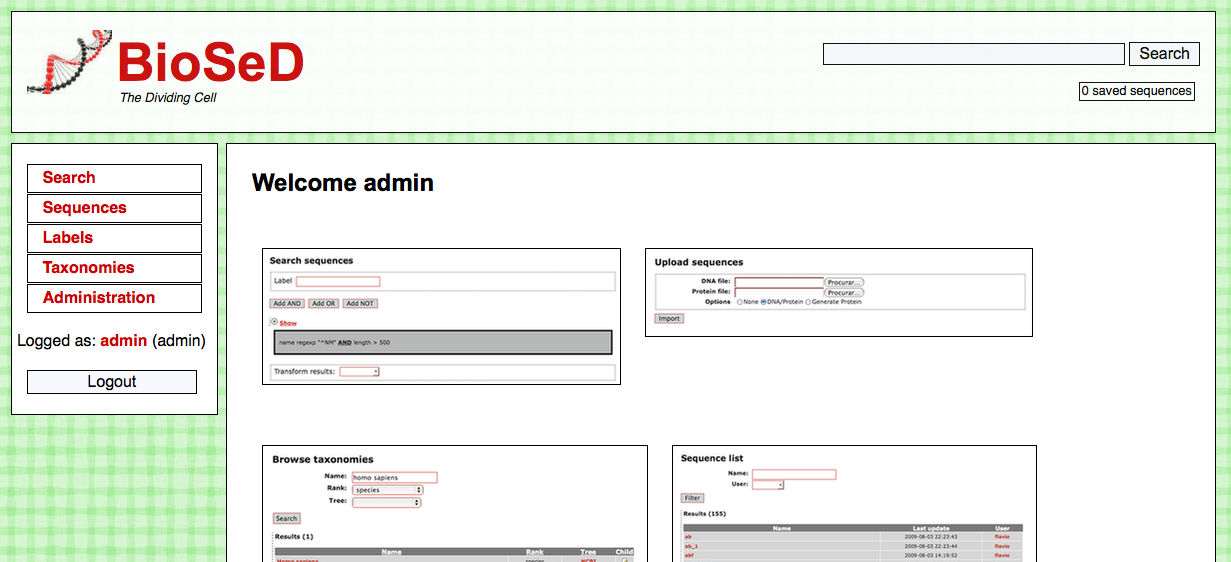
\includegraphics[scale=0.35]{interface.png}
  \caption{System home page.}
  \label{fig:home_page}
\end{figure}

For the rest of this section, we will describe the most interesting
user interface components and interactions.

\section{Grid component}

The grid component is one of the most used interface components in the application.
It works as component to display lists of things. It was implemented as a full jQuery plugin (jquery.mygrid.js).

It supports: custom columns, cell clicking, cell links, column hiding, pagination, cell edition,
row remotion, whole grid reload and row highlighting. More importantly, the data it uses to display the grid
can be fetched from the server (local data is also supported) and used dynamically with pagination.

An usage example is shown in Listing \ref{grid_usage}.

\begin{lstlisting}[float, language=html, frame=single, label=grid_usage, caption={Grid component usage.}]
$('#user_list')
  .gridEnable({paginate: false})
  .grid({
    url: get_app_url() + '/profile',
    retrieve: 'get_all',
    fieldNames: ['Name', 'Complete name', 'Email', 'Last access'],
    fields: ['name', 'complete_name', 'email', 'last_access'],
    width: {
      name: w_user,
      email: w_email,
      last_access: w_update
    },
    links: {
      name: function (row) {
        return get_app_url() + '/profile/view/' + row.id;
      }
    }
  });

(...)

<div id="user_list"></div> <!-- the grid is placed in div #user_list -->
\end{lstlisting}

To see how a grid can look like please see Figure \ref{fig:grid_component}.
The example lists all system labels.

\begin{figure}[H]
  \centering
    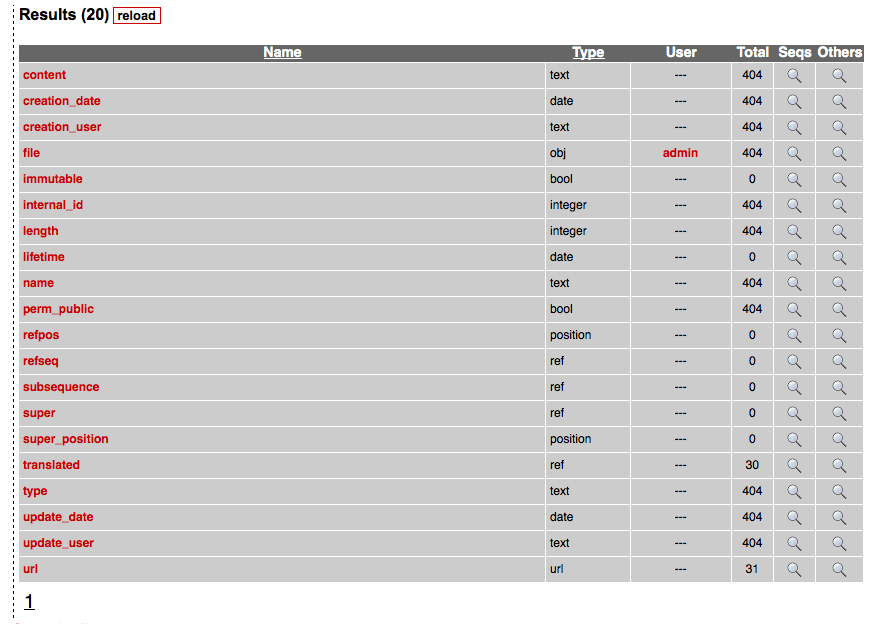
\includegraphics[scale=0.5]{grid.png}
  \caption{Grid component aspect.}
  \label{fig:grid_component}
\end{figure}

\section{Query interface}

The search screen is probably the most important page in the whole application.
This search page helps the user build the query expression and can display the results
in real time.
It is structured into three parts: query input, results and operations.

A search screen showing the query input component is shown in Figure \ref{fig:search1}.

To build a query the user must input the label name, operator and value and then
select in which part of the search tree this new term will be placed. AND, NOT and OR
operators can also be inserted. Optionally, one can also reset the whole query expression.

The query expression is shown in two formats: tree like and simple text. When selecting
a term in the tree format the user can delete that sub-query. The simple text format is read-only.
Optionally we can also transform query results by selecting a reference label from te \textbf{Transform results}
list.

Every time the query expression changes, we store it in a cookie. When the search page
is opened again the old query is restored. This proves useful when the user goes back
and forth between the search page and each operation page, without losing any work. 

\begin{figure}[H]
  \centering
    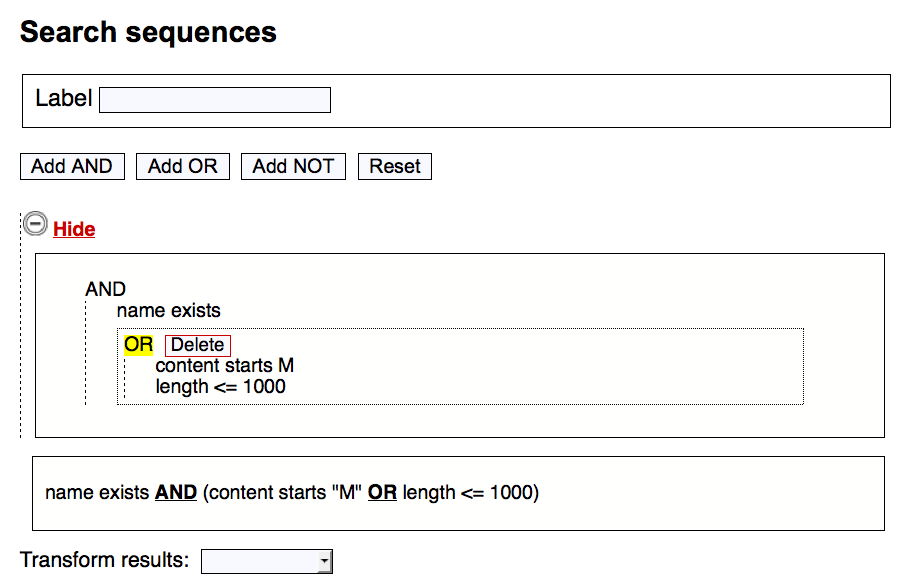
\includegraphics[scale=0.5]{search1.png}
  \caption{Search query input.}
  \label{fig:search1}
\end{figure}

The preview component initially shows the result total, but can display the complete result set
that match the query in a grid component.
The grid component can be augmented with label instance information in \textbf{View label}. For
example we could input the \textbf{length} label and then the grid will show the length for each
sequence in the list.

\begin{figure}[H]
  \centering
    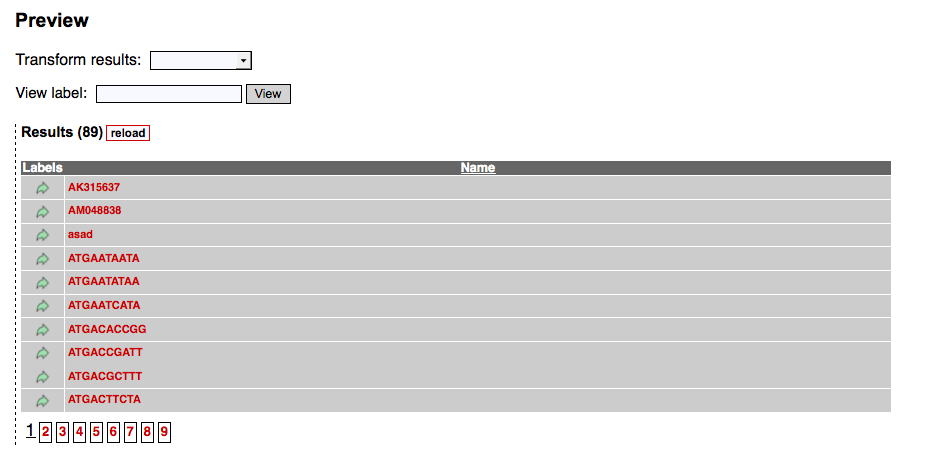
\includegraphics[scale=0.5]{search3.png}
  \caption{Search preview results.}
  \label{fig:search3}
\end{figure}

Appearing right below the preview component, the operator component is shown in Figure \ref{fig:search2}.

\begin{figure}[H]
  \centering
    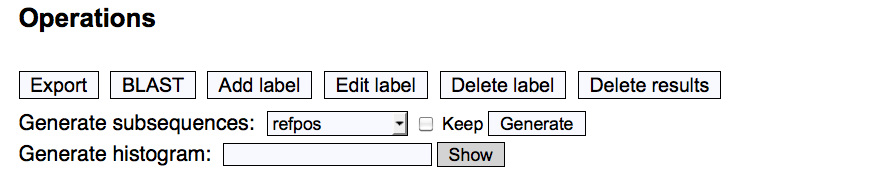
\includegraphics[scale=0.5]{search2.png}
  \caption{Search operations.}
  \label{fig:search2}
\end{figure}

The following operations are available:

\begin{itemize}
  \item \textbf{Export}: export the result sequence list to a file.
  \item \textbf{BLAST}: run a BLAST search across the result list.
  \item \textbf{Add label}: adds label instances to all sequences in the result list.
  \item \textbf{Edit label}: same as before, but editing.
  \item \textbf{Delete label}: removes a specific label from the result list sequences.
  \item \textbf{Delete results}: simply delete the result list sequences.
  \item \textbf{Generate subsequences}: can generate sub-sequences using a \textbf{position} label and the current result list. The user has the option to keep the new subsequences around or not.
  \item \textbf{Generate histogram}: generate an histogram analysis based on the input label. When the label
  is numeric and multiple the user can choose a representative value for each sequence: minimum, maximum or average.
\end{itemize}

Finally, three search screens are available: one can use all sequences, other only searches in DNA sequences and
the third in protein sequences. Hopefully, the interface looks the same in all of them. 

\section{Written query interface}

On the top of each page there is a search box (Figure \ref{fig:search_box}) that can receive various kinds of input.
The user can input query expressions like $<$\textit{(length $>$ 500 and name exists) or content regexp AGTG}$>$
or some other text for system wide searches.

\begin{figure}[H]
  \centering
    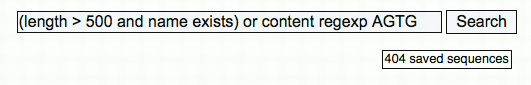
\includegraphics[scale=0.7]{search_box.png}
  \caption{Search box.}
  \label{fig:search_box}
\end{figure}

When the server receives the POST query it tries to parse the expression as a query expression,
if it fails the server will search across all system objects and display, in a different page,
all the objects in which the text matched.

The objects used in this query are:

\begin{itemize}
  \item labels
  \item ranks
  \item taxonomies
  \item sequences
\end{itemize}

This feature is useful to search the system in a fuzzy like way. For example, if the user types
'homo sapiens' in the box, the system will potentially display all taxonomies
that contain 'homo sapiens', as shown in Figure \ref{fig:wide_search}.

\begin{figure}[H]
  \centering
    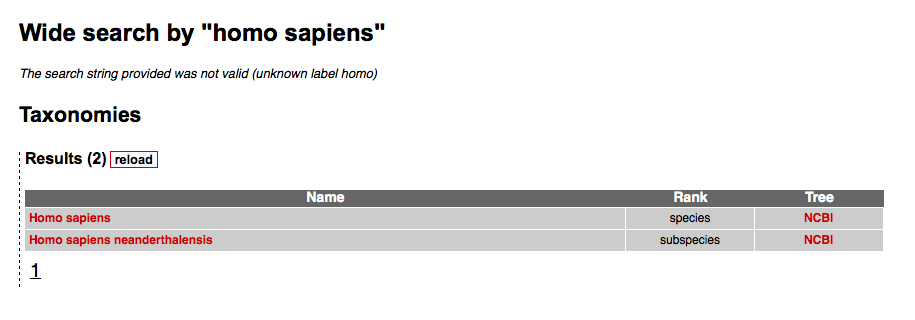
\includegraphics[scale=0.5]{wide_search.png}
  \caption{Wide search page.}
  \label{fig:wide_search}
\end{figure}

\section{Sequence}

A new sequence can be inserted into the system by providing its name and content, as
shown in Figure \ref{fig:add_sequence}.

When the new sequence is DNA, an option named
\textbf{Generate protein} can be checked to generate
the respective protein sequence and link the DNA sequence with the translated protein.

\begin{figure}[ht]
  \centering
    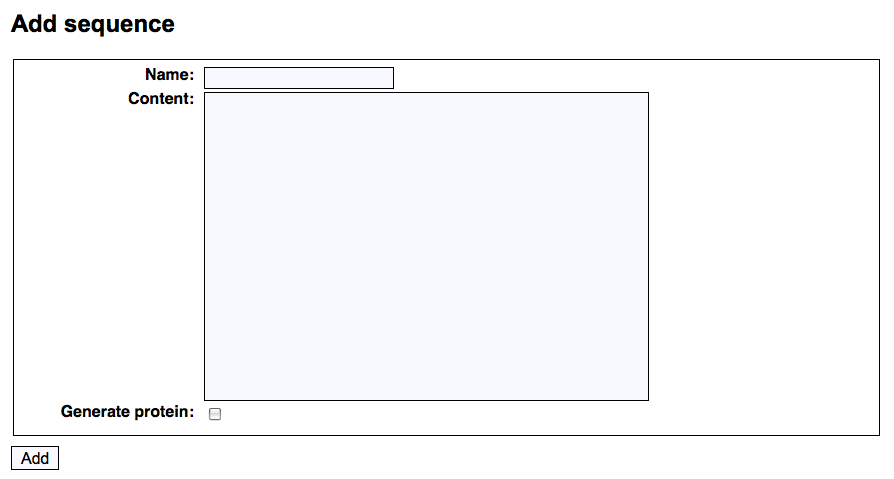
\includegraphics[scale=0.5]{add_sequence.png}
  \caption{Add new sequence page.}
  \label{fig:add_sequence}
\end{figure}

Once the sequence is added the user is redirected to the sequence's page, where
sequence's name, content and history information is shown. A button named
\textbf{View Labels} is available to access the sequence labels page.

The labels page displays the sequence's annotated labels, labels available to add,
missing labels and non-multiple labels that have more than one instance for this sequence,
which we name the \textbf{bad multiple} labels.

The annotated labels list is always shown. The \textbf{Available} labels list
is only shown if the sequence is not annotated with every system label, which is the most frequent case.
The missing labels list is only shown if the sequence has not been annotated with
mandatory labels, like \textbf{type} or \textbf{length}. The bad multiple labels list
is only shown when, for some reason, the sequence is annotated with various instances of
the same label that is not multiple, this can happen when a label, once multiple, no longer is.

An example labels page in shown in Figure \ref{fig:labels}. Some sets of labels are not shown
by default and must be displayed by clicking \textbf{Show}. Filtering of labels is also available
as shown in the example page.

\begin{figure}[ht]
  \centering
    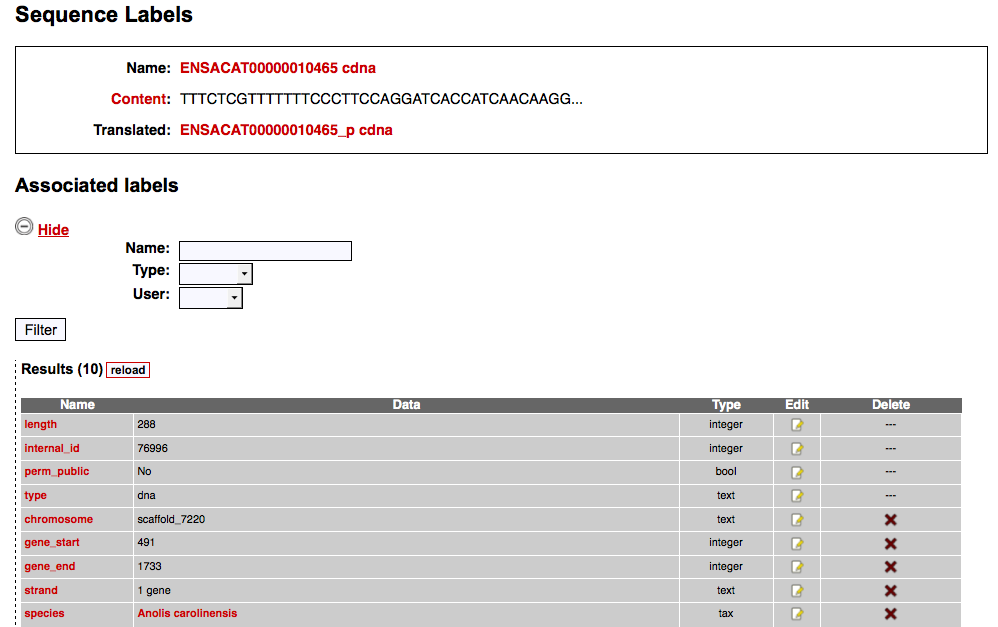
\includegraphics[scale=0.5]{labels.png}
  \caption{Example labels page.}
  \label{fig:labels}
\end{figure}

Some useful interactions were implemented: clicking in one missing label opens the available pages
separator and highlights the label there, easing the process of annotating the sequence with missing
labels; clicking in one bad-multiple label highlights the specific label instance in the annotated labels list.

\section{Changing sequence labels}

To annotate a sequence with new label instances, the user must go to the available labels list \ref{fig:available_labels}
and click the \textbf{add} icon. A new window appears to input the label instance value.

If the label supports automatic generation a checkbox named \textbf{Generate default value} is displayed.
If checked in, the result will be a new label instance generated from the label code.

\begin{figure}[ht]
  \centering
    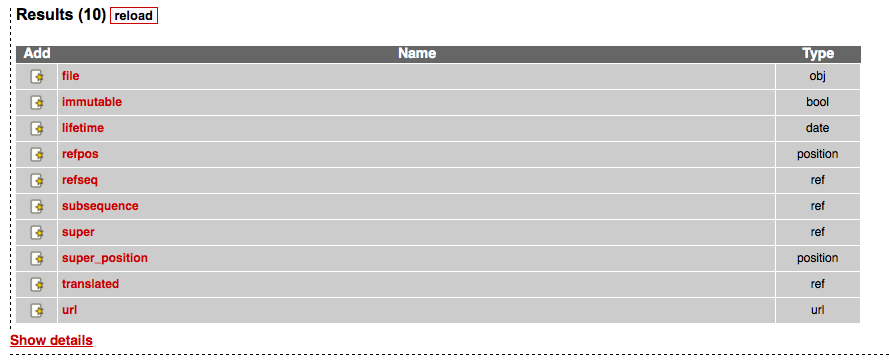
\includegraphics[scale=0.5]{available_labels.png}
  \caption{Available labels grid.}
  \label{fig:available_labels}
\end{figure}

For each label type, this screen is slightly different. Here's a summary:

\begin{itemize}
  \item \textbf{integer}, \textbf{float}: text field with numeric validation.
  \item \textbf{text}: simple text field.
  \item \textbf{url}: text field with URL validation.
  \item \textbf{bool}: a checkbox.
  \item \textbf{position}: two text fields with numeric validation.
  \item \textbf{taxonomy}: a searchable grid with taxonomies that can be selected.
  \item \textbf{reference}: a searchable grid with sequences that can be selected.
  \item \textbf{date}: text field with calendar widget.
  \item \textbf{object} (Figure \ref{fig:obj_label}): if the label has files attached a select list is displayed containing them.
  An upload field is also available.
\end{itemize}

\begin{figure}[ht]
  \centering
    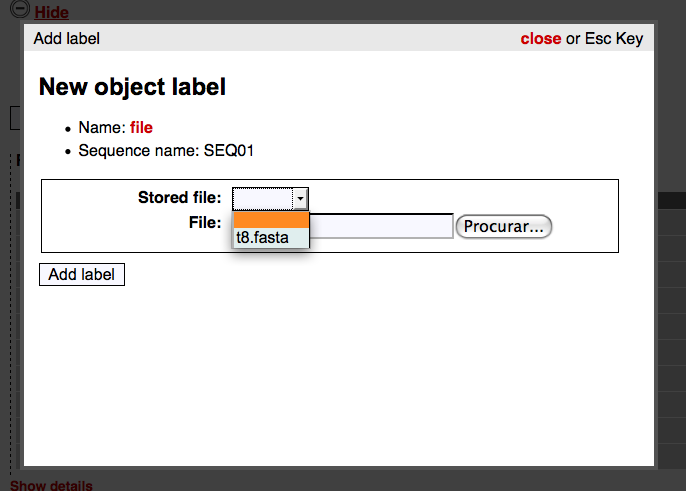
\includegraphics[scale=0.5]{obj_label.png}
  \caption{Annotating a new object label.}
  \label{fig:obj_label}
\end{figure}

To edit label instances, the process is similar, but uses the annotated labels list. Once a label instance
is added or edited the page is updated to reflect the changes.

\section{Batch uploading}

The application features a page where the user can upload sequence files and have them
imported into the system.

In this page (Figure \ref{fig:sequence_upload}) three options are available:
upload a single file; upload both DNA and protein file, linking
the sequences along the process; upload a DNA file and also generate protein sequences.
When generating protein sequences, it is possible to keep the FASTA annotated information,
thus annotating the protein sequences with the DNA labels.

\begin{figure}[ht]
  \centering
    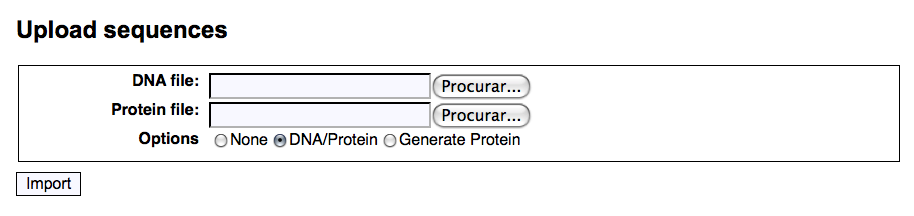
\includegraphics[scale=0.5]{sequence_upload.png}
  \caption{Upload sequences page.}
  \label{fig:sequence_upload}
\end{figure}

Once the files are uploaded and processed, a new page appears reporting the process (Figure \ref{fig:batch_report}).
In this page, the status for each sequence found is displayed, if it was inserted or not, the label metadata found, if any,
and the status for each annotated sequences labels.

If the system found any empty sequences, then they are reported in this page. The system
also creates query expressions to query the uploaded sequences, which can be useful to run
various kinds of operations against the imported sequences.

\begin{figure}[ht]
  \centering
    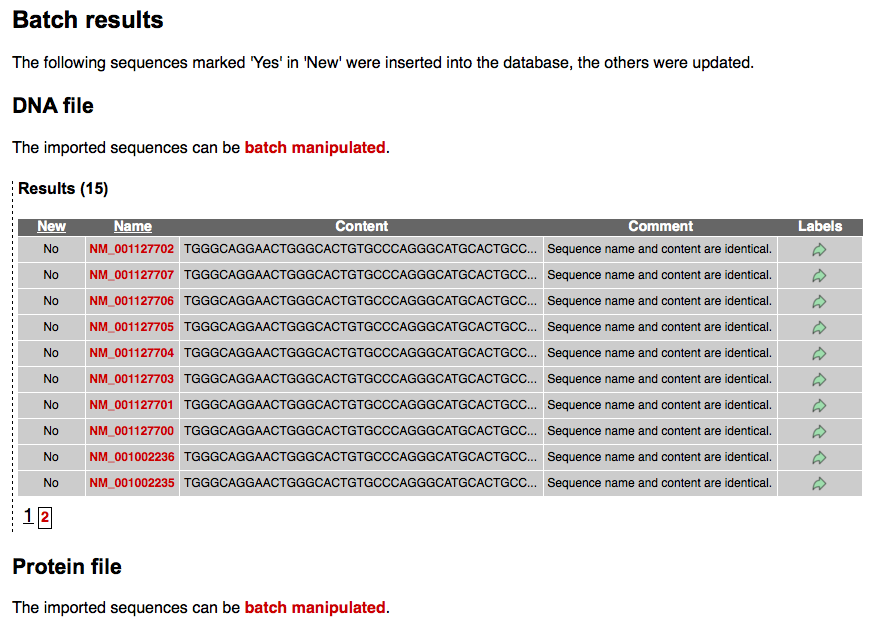
\includegraphics[scale=0.5]{batch_report.png}
  \caption{Upload report after sending a pair of DNA and protein files.}
  \label{fig:batch_report}
\end{figure}

\section{Taxonomy tree browsing}

Once the user selects a tree to browse from the system's taxonomy tree list, he can
navigate through the tree, selecting nodes or going up in the hierarchy.
This page also features a breadcrumb component, enabling the user to jump to a certain
ancestor.

Every navigation step is done without page refreshes. An example page is shown in
Figure \ref{fig:tree_browse}.

\begin{figure}[ht]
  \centering
    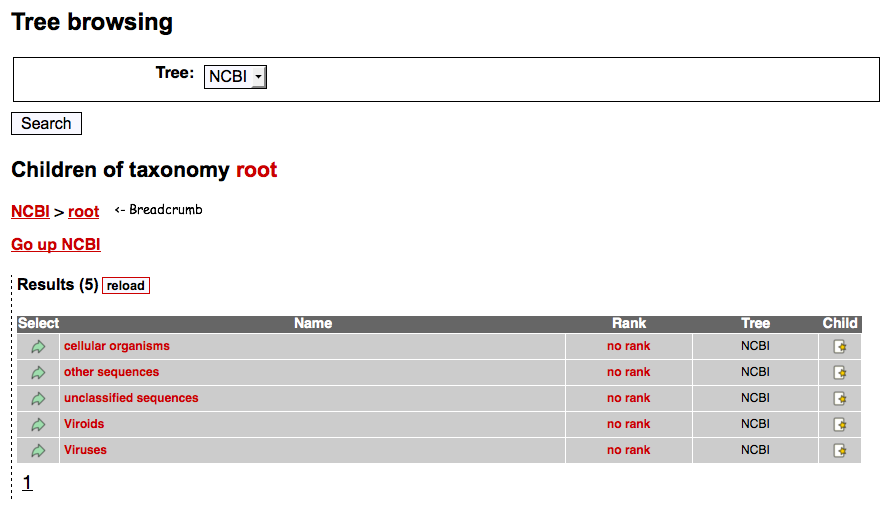
\includegraphics[scale=0.5]{tree_browsing.png}
  \caption{Navigating through the NCBI tree.}
  \label{fig:tree_browse}
\end{figure}

\section{Histograms}

Histograms are useful to analyze a label's value distribution across a set of sequences.
To display a histogram we implemented a jQuery plugin (file \textit{jquery.plot.js}). This plugin
accepts a javascript object representing the value distribution and creates HTML for the plot.

This plugin makes use of the width CSS property to display variable sized plot bars.
An example plot bar is displayed in Figure \ref{fig:histogram}.

\begin{figure}[ht]
  \centering
    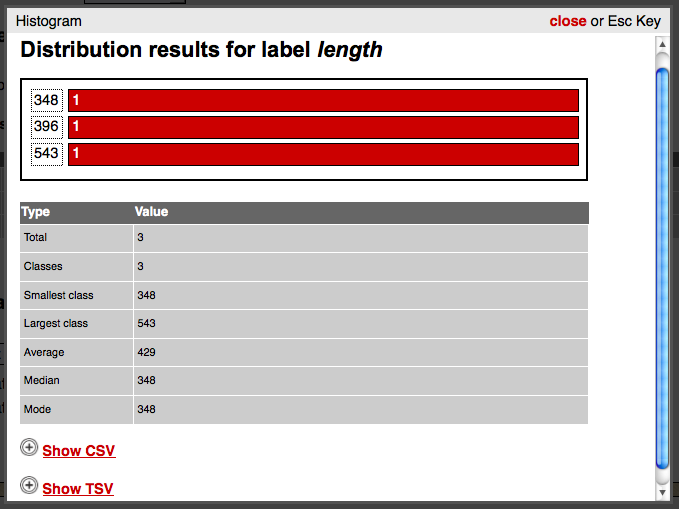
\includegraphics[scale=0.5]{histogram.png}
  \caption{Plotting histograms.}
  \label{fig:histogram}
\end{figure}

\section{BLAST}

The BLAST search interface provides a page where the query sequences
can be provided and the BLAST parameters can be tuned before launching
the search.

This page is displayed on Figure \ref{fig:blast} and shows two distinct
sections: section (1) for basic BLAST setup, section (2) for advanced parametrization.

\begin{figure}[ht]
  \centering
    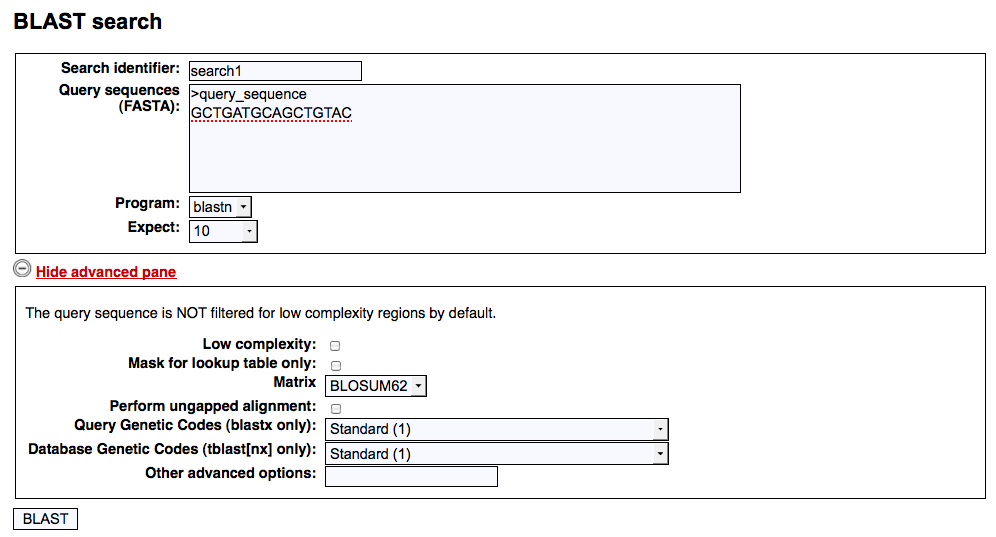
\includegraphics[scale=0.45]{blast.png}
  \caption{BLAST search screen.}
  \label{fig:blast}
\end{figure}

In the first section, the user must provide a search identifier, which identifies
this specific search and the query sequences in FASTA format that will be
matched against the result sequence list. It is also possible to
select between specialized BLAST programs, depending on the result sequence list
characteristics, but usually this option is pretty restricted by the system knowledge of
the sequences. Finally, the default \textit{expect} value can be changed to best
suit the search purposes.

The second section provides more advanced BLAST options.
If some BLAST option can not be found, the \textbf{Other advanced options} input box
is provided to pass arbitrary \texttt{blastall} program arguments.

Once the BLAST parameters are set, the \textbf{BLAST} button launches the BLAST
search and a new page is loaded (Figure \ref{fig:blast_results}), presenting the BLAST output and a button to,
optionally, annotate the matched sequences with BLAST information.

\begin{figure}[ht]
  \centering
    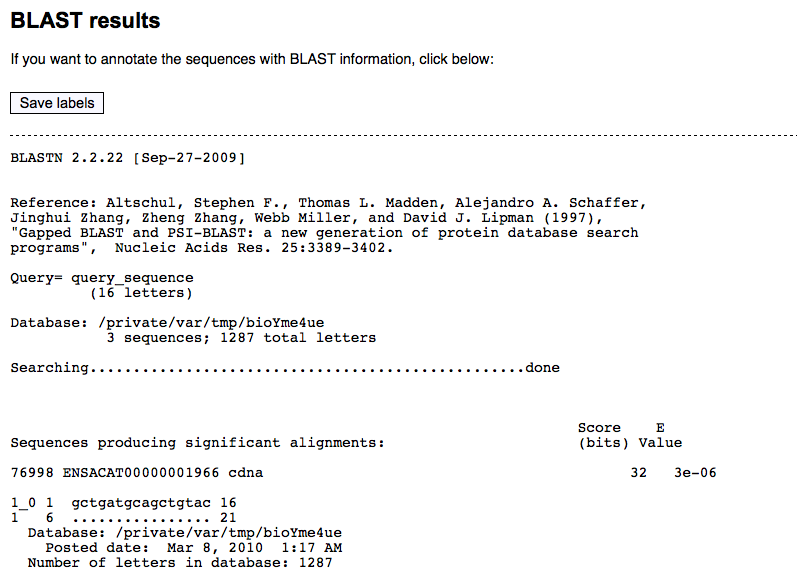
\includegraphics[scale=0.45]{blast_results.png}
  \caption{BLAST results screen.}
  \label{fig:blast_results}
\end{figure}

\section{Loading screens}

For long server processing tasks and to give the user some feedback, we used the jquery blockUI
plugin to implement loading screens.

These loading screens are used in three occasions: when uploading sequence files, when annotating sequences
in batch or when editing label instances in batch.

For each loading screen and associate form we associate a random event code. This code is sent
along the data to process and is used by the server to update the event status into the database.
The client uses the event code to poll the server for information about the specific event. When requested,
the server returns HTML about the event, which is displayed in the loading screen.

An example loading screen (for sequence upload) is displayed in Figure \ref{fig:loading_screen}.

\begin{figure}[ht]
  \centering
    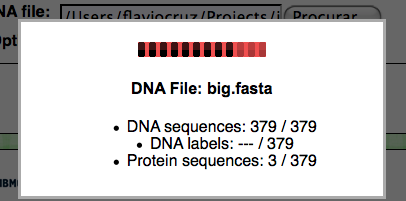
\includegraphics[scale=0.5]{loading_screen.png}
  \caption{Example loading screen.}
  \label{fig:loading_screen}
\end{figure}

Loading screens give an extra clue for when the server will complete the request
and can prevent users from wondering if the server stopped responding or if the request
was sent at all, among other problems.

\clearpage
\chapter{Results}

We next present some experimental results concerning time and space efficiency of various parts of the system.
For our experiments we will feed scripted tasks into the server. No network latency will be involved
as the scripts will be run directly in the server.

The environment for running our scripts is composed of the following components:

\begin{itemize}
  \item Processor: 2GHz Intel Core 2 Duo
  \item Memory: 2GB 1067 MHz DDR 3
  \item Disk: 160GB 5400RPM
  \item Operating System: MacOSX 10.5
  \item MySQL 14.14 Distrib 5.1.32, for apple-darwin9.5.0 (i386)
  \item Apache 2.2.13
  \item PHP 5.3.0
\end{itemize}

To measure time and space results, we considered three main functionalities:

\begin{itemize}
  \item Sequence import: Importing sequences into the system using the FASTA format is an important
  functionality and can be very time consuming. It is an important metric for how fast the system
  can insert new sequences, check existing annotation and update sequence annotations.
  \item Multiple sequence annotation: batch inserting or editing of label instances can give us some
  important insights on annotation performance.
  \item Search: Being the system core functionality it is important to measure its efficiency.
\end{itemize}

Time is measured by calculating the number of seconds and milliseconds spent executing the operation.
For space measurements, we compute the database size using the SQL query presented in Listing \ref{mysql_database_size}.

\begin{lstlisting}[float, language=sql, frame=single, label=mysql_database_size, caption={MySQL database size query.}]
SELECT table_schema "Data Base Name", sum( data_length + index_length) / 1024 "Data Base Size in KB" FROM information_schema.TABLES WHERE table_schema = "BioSeD_Database";
\end{lstlisting}

\section{Sequence import}

Every FASTA file used in this section is available in the source code package at \textit{fasta/}.

The scripts used to import sequence files were:

\begin{itemize}
  \item tools/import\_seq\_file.sh: simple file import.
  \item tools/import\_and\_generate.sh: import a DNA file and generate proteins.
  \item tools/import\_two.sh: import a pair of DNA and protein files.
\end{itemize}

The test files used were:

\begin{itemize}
  \item fasta/big.fasta: 373 DNA sequences and 10 associated labels. 6 repeated sequences. All labels described in the file were installed in the system.
  \item fasta/serpina1.dna.fasta and fasta/serpina1.trans.fasta: pair of DNA and protein files, 15 sequences each. No labels.
\end{itemize}

The labels installed in the system during measurements are available in \textit{fasta/test\_labels.xml}.
Initial database size was 803.0664KB. The tables were recreated before each test using \texttt{OPTIMIZE TABLE}.

\begin{table}[H]
  \begin{center}
    \scalebox{0.7}{
    \begin{tabular}{ | l | c | c | c | c | }
      \hline
      \textbf{Test} & \textbf{Sequences in the system} & \textbf{Time} & \textbf{Database size} & \textbf{Size increment} \\ \hline
      (1) big.fasta with no protein translation & 0 & 0m28.139s & 2819.0664KB & 2015.9996KB \\ \hline
      (2) big.fasta with protein translation & 0 & 1m0.126s & 4739.0664KB & 3936KB \\ \hline
      (3) serpina1.dna.fasta + serpina1.trans.fasta & 0 & 0m2.058s & 883.0664KB & 80KB \\ \hline
      (4) serpina1.dna.fasta + serpina1.trans.fasta & 748: test (2) results & 0m2.017s & 4835.0664KB & 4032KB \\ \hline
    \end{tabular}}
  \end{center}
  \caption{Sequence importing results.}
  \label{tbl:results_importing}
\end{table}

By analyzing Table \ref{tbl:results_importing} we can see that the number of sequences to import linearly affects the
resulting time and space. For example, when importing translated sequences in the test (2), the test time nearly doubled from
a simple import from the test (1).

\section{Multiple sequence annotation}

For multiple sequence annotation we loaded the system with hundreds of sequences and then
batch annotated them.

The labels used in these tests are \textbf{url} (an URL multiple label) and \textbf{refpos} (a position label).

The scripts we used to run the tests were:

\begin{itemize}
  \item tools/add\_url\_label.sh
  \item tools/add\_refpos\_label.sh
  \item tools/edit\_refpos\_label.sh
\end{itemize}

The database state from sequence importing test (4) was used and the initial database size was 4835.0664KB.

\begin{table}[H]
  \begin{center}
    \scalebox{0.7}{
    \begin{tabular}{ | l | c | c | c | c | }
      \hline
      \textbf{Test} & \textbf{Sequences} & \textbf{Time} & \textbf{Database size} & \textbf{Size increment} \\ \hline
      (1) annotate all sequences with \textbf{url} (google.pt, parameter google) & 788 & 0m4.291s & 5091.0664KB & 256KB \\ \hline
      (2) annotate all sequences with \textbf{url} (sapo.pt, parameter sapo) & 788: test (1) & 0m4.318s & 5491.0664KB & 656KB \\ \hline
      (3) annotate all sequences with \textbf{refpos} (start: 1, length: 10) & 788: test (2) & 0m4.453s & 5683.0664KB & 848KB \\ \hline
      (4) edit all \textbf{refpos} instances (start: 2, length: 10) & 788: test (3) & 0m7.246s & 5811.0664KB & 976KB \\ \hline
    \end{tabular}}
  \end{center}
  \caption{Multiple sequence annotation.}
  \label{tbl:results_multiple_annotation}
\end{table}

The results can be seen in Table \ref{tbl:results_multiple_annotation}.
Some conclusions can be made:

\begin{itemize}
  \item Editing label values takes more time than adding them, as the edit operations requires
  more verifications.
  \item As we annotate the sequences with more labels, more time is needed to verify that we are not
  repeating label values. More annotations also means searching through larger database tables.
\end{itemize}

\section{Search}

For search we created the script tools/search.sh, which accepts a search expression and, optionally, a transform label.

First, we used a sequence set composed of serpina1.dna.fasta, serpina1.trans.fasta and big.fasta without DNA translation
(409 sequences). The NCBI taxonomy database was imported into the system.
Next, we ran some test expressions against the database and augmented it with big.fasta protein translations and ran
the same test expressions.

\begin{table}[H]
    \begin{tabular}{ | p{11.2cm} | c | c |}
      \hline
      \textbf{Expression} & \textbf{Results} & \textbf{Time} \\ \hline
      length exists & 409 & 0m0.150s \\ \hline
      length $>$ 0 & 409 & 0m0.152s \\ \hline
      length $>$ 0 and name regexp A & 48 & 0m0.134s \\ \hline
      length $>$ 0 and name regexp A and content regexp A & 48 & 0m0.137s \\ \hline
      length $>$ 0 and name regexp A and content regexp A and species like Drosophila & 44 & 0m5.491s \\ \hline
  \end{tabular}
  \caption{Searching 404 sequences, no result translation.}
  \label{tbl:results_search_404_no_translation}
\end{table}

\begin{table}[H]
    \begin{tabular}{ | p{11.2cm} | c | c |}
      \hline
      \textbf{Expression} & \textbf{Results} & \textbf{Time} \\ \hline
      length exists & 30 & 0m0.125s \\ \hline
      length $>$ 0 & 30 & 0m0.134s \\ \hline
      length $>$ 0 and name regexp A & 4 & 0m0.129s \\ \hline
      length $>$ 0 and name regexp A and content regexp A & 4 & 0m0.131s \\ \hline
      length $>$ 0 and name regexp A and content regexp A and species like Drosophila & 0 & 0m1.396s \\ \hline
  \end{tabular}
  \caption{Searching 404 sequences with \textbf{translated} translation.}
  \label{tbl:results_search_404_translation}
\end{table}

\begin{table}[H]
    \begin{tabular}{ | p{11.2cm} | c | c |}
      \hline
      \textbf{Expression} & \textbf{Results} & \textbf{Time} \\ \hline
      length exists & 788 & 0m0.352s \\ \hline
      length $>$ 0 & 788 & 0m0.170s \\ \hline
      length $>$ 0 and name regexp A & 244 & 0m0.145s \\ \hline
      length $>$ 0 and name regexp A and content regexp A & 244 & 0m0.304s \\ \hline
      length $>$ 0 and name regexp A and content regexp A and species like Drosophila & 44 & 0m2.799s \\ \hline
  \end{tabular}
  \caption{Searching 788 sequences with no translation.}
  \label{tbl:results_search_778_no_translation}
\end{table}

\begin{table}[H]
    \begin{tabular}{ | p{11.2cm} | c | c |}
      \hline
      \textbf{Expression} & \textbf{Results} & \textbf{Time} \\ \hline
      length exists & 788 & 0m0.188s \\ \hline
      length $>$ 0 & 788 & 0m0.178s \\ \hline
      length $>$ 0 and name regexp A & 244 & 0m0.298s \\ \hline
      length $>$ 0 and name regexp A and content regexp A & 244 & 0m0.163s \\ \hline
      length $>$ 0 and name regexp A and content regexp A and species like Drosophila & 43 & 0m2.827s \\ \hline
  \end{tabular}
  \caption{Searching 778 sequences with \textbf{translated} translation.}
  \label{tbl:results_search_778_translation}
\end{table}

From tables \ref{tbl:results_search_404_no_translation}, \ref{tbl:results_search_404_translation},
\ref{tbl:results_search_778_no_translation}, and \ref{tbl:results_search_778_translation}
we can see that the number of stored sequences affects the system performance.
The performance also tends to decrease when the search expression gets more complex.

\clearpage
\chapter{Conclusion}

In this technical report we presented a possible design and implementation of a bioinformatics
system that was built to store sequences and annotations called labels.

We presented all the system objects that make up the bulk of the system: sequences, labels and taxonomies.

The design of a relational model with an emphasis on search facilities was put forward in the design section along
with data formats and a query grammar. The query grammar, used for sequence searching, showed how search fits in the system.
The main difficulty when designing the system was coming up with the relational model and making it efficient to
store and retrieve thousands of rows of data, especially when using the NCBI database.

The implementation section explained how the queries are processed and run in an efficient manner
using the MySQL database. Some database optimizations were listed and explained: indexes, views and keys.
We build a query expression parser that is capable of parsing the grammar put forward in the design section.
The parser helped turning query expressions into query objects and finally transforming them in efficient SQL code.
In terms of difficulties, \textit{CodeIgniter} had some problems when running multiple SQL queries;
the Database plugin was caching all the queries, wasting a lot of memory.
Another problem was related to cookie handling and encoding, mainly when storing
regular expressions in cookies and some characters were lost during the encoding/decoding
process.

The most interesting aspects of our user interface were displayed and described. Two types of
search interfaces were designed: one more exploratory oriented, where you build the search expressions
step by step and view the results in realtime and where each sub-expression can be analyzed; and another form of
search, for more experienced users, where the expressions are written directly.
The designed search page provides an interesting analysis and operation facility, making it easy to generate
histograms for label distribution and run various tasks in a batch fashion over the result list.

Some project difficulties involved the recurrent problem in software engineering, which is the change of
requirements during the project lifetime.
More frequent and intensive testing were not always done and it caused some problems. The creation
of a set of unit and interface tests should have been done to fight those issues.

We also made some benchmarking for the most interesting features: searching, sequence importing and multiple sequence annotation.

We conclude this report believing that the resulting system will be useful for sequence management and analysis,
making the life easier for those who work with the system.

\clearpage
\renewcommand{\bibname}{References} 
\begin{thebibliography}
  {10}
	\bibitem{apache} The Apache Software Foundation, \url{http://www.apache.org/}
	
	\bibitem{mysql} MySQL, Sun Microsystems, \url{http://www.mysql.com/}
	
	\bibitem{json} JavaScript Object Notation, \url{http://json.org/}
	
	\bibitem{php} PHP: HyperText Preprocessor, \url{http://www.php.net/}
	
	\bibitem{innodb} The InnoDB Storage Engine, \url{http://dev.mysql.com/doc/refman/5.0/en/innodb.html}
	
	\bibitem{fasta} FASTA format description, \url{http://www.ncbi.nlm.nih.gov/blast/fasta.shtml}
	
	\bibitem{codeigniter} CodeIgniter - Open Source PHP web application framework, \url{http://codeigniter.com/}
	
	\bibitem{smarty} Smarty : Template Engine, \url{http://www.smarty.net/}
	
	\bibitem{jquery} jQuery: The Write Less, Do More, Javascript Library, \url{http://jquery.com/}
	
	\bibitem{python} Python Programming Language, \url{http://www.python.org/}
	
	\bibitem{mysqldb} MySQLdb's User Guide, \url{http://mysql-python.sourceforge.net/MySQLdb.html}
	
	\bibitem{emboss} Rice, P. Longden, I. and Bleasby, A. EMBOSS: The European Molecular Biology Open Software Suite.
	\textit{Trends in Genetics} 16, (6) pp276--277, 2000.
	
	\bibitem{compilers} Aho, Sethi, Ullman, Compilers: Principles, Techniques, and Tools, Addison-Wesley, 1986. ISBN 0-201-10088-6
	
	\bibitem{seqret} seqret, EMBOSS, \url{http://emboss.sourceforge.net/apps/release/5.0/emboss/apps/seqret.html}
	
	\bibitem{ncbi} NCBI website, \url{http://www.ncbi.nlm.nih.gov/}
	
	\bibitem{ncbi_tax} NCBI taxonomy database, \url{ftp://ftp.ncbi.nih.gov/pub/taxonomy/}
	
	\bibitem{genotator} Harris, N.L. Genotator: A workbench for sequence annotation. \textit{Genome Research} 7(7):754-762, 1997.
	
	\bibitem{about_genotator} Harris, N.L. About Genotator, \url{http://www.fruitfly.org/~nomi/genotator/about.html}
	
	\bibitem{biodas} Dowell RD, Jokerst RM, Day A, Eddy SR, and Stein L. The distributed annotation system.
	\textit{BMC Bioinformatics 2001}; 2 7. pmid:11667947, 2001.
	
	\bibitem{about_biodas} BioDAS project. About DAS, \url{http://www.biodas.org/wiki/Main_Page}
	
	\bibitem{ensembl} Ensembl project, How Ensembl uses DAS, \url{http://www.ensembl.org/info/data/ensembl_das.html}
	
	\bibitem{gbrowse} Stein LD et al. The generic genome browser: a building block for a model organism system database. \textit{Genome Res 12: 1599-610}, 2002.
	
	\bibitem{igb} Integrated Genome Browser, \url{http://genoviz.sourceforge.net/}
	
	\bibitem{ensmart_shopping} D. Gilbert, Shopping in the genome market with EnsMart, \textit{Briefings in Bioinformatics}, 2003.
	
	\bibitem{ensmart} Kasprzyk A, Keefe D, Smedley D, London D, Spooner W, Melsopp C, Hammond M, Rocca-Serra P, and Cox T, Birney E. EnsMart: a generic system for fast and flexible access to biological data. \textit{European Bioinformatics Institute}, 2004.
  
  \bibitem{biomart} Smedley D, Haider S, Ballester B, Holland R, London D, Thorisson G, Kasprzyk A. BioMart--biological queries made easy. \textit{BMC Genomics}, 2009.
  
  \bibitem{cbs} Peter F. Hallin and David W. Ussery. CBS Genome Atlas Database: a dynamic storage for bioinformatic results and sequence data. \textit{Bioinformatics} Volume 20 Issue 18, 2004.
	
	\bibitem{extensible_open_source} Sean D. Mooney and Peter H. Baenziger. Extensible open source content management systems and frameworks: a solution for many needs of a bioinformatics group. \textit{Center for Computational Biology and Bioinformatics, Department of Medical and Molecular Genetics, Indiana University School of Medicine}, 2007.
	
	  \bibitem{gendb} Folker Meyer, Alexander Goesmann, Alice C. McHardy, Daniela Bartels, Thomas Bekel, Jorn Clausen, Jorn Kalinowski, Burkhard Linke, Oliver Rupp, Robert Giegerich and Alfred Puhler. \textit{GenDB: an open source genome annotation system for prokaryote genomes}. \textit{Nucleic Acids Research}, 2003.
	  
	  \bibitem{blast} Altschul, S.F., Gish, W., Miller, W., Myers, E.W. and Lipman, D.J. \textit{Basic local alignment search tool}. \textit{Journal of Molecular Biology}, 1990.
	  
\end{thebibliography}

\appendix

\chapter{User manual}

\section{Installation}

Before installing the application we will need to download the install package from the project
webpage. Two methods are available to download the application: downloading a release or
through Subversion, getting the most recent source code updates and fixes.

First, point your browser to \url{http://code.google.com/p/ibmc-bio-db/}.

If you want to use Subversion, select \textbf{Source} and once the page has loaded
you should see the Subversion checkout command. Run:

\begin{lstlisting}[language=c, frame=single]
$ svn checkout http://ibmc-bio-db.googlecode.com/svn/trunk/ biosed
\end{lstlisting}

If you want to download a stable release, select \textbf{Downloads} and click on the most up-to-date
version. Once the file as downloaded, run:

\begin{lstlisting}[language=c, frame=single]
$ tar zxvf biosed-version.tar.gz
\end{lstlisting}

For both methods, enter into the \textbf{biosed} directory. Take a look at the file \textbf{README}
and follow the instructions.

Once done, the application should be installed. Congratulations!

The install scripts creates one user for using the application, the \textit{admin} user, and, as name
says has more rights than \textit{normal} users.
Right now, you should point your browser to the application's location and login with this user.

Once the page has loaded, you should now see the main application's page.
On the left is the main menu, in the header there is a search box and at the main box is located
the main application's work area.

Right below the main menu there is a login box. Put \textit{admin} in the user field and
use the password you provided during the installation process.

\begin{figure}[H]
  \centering
    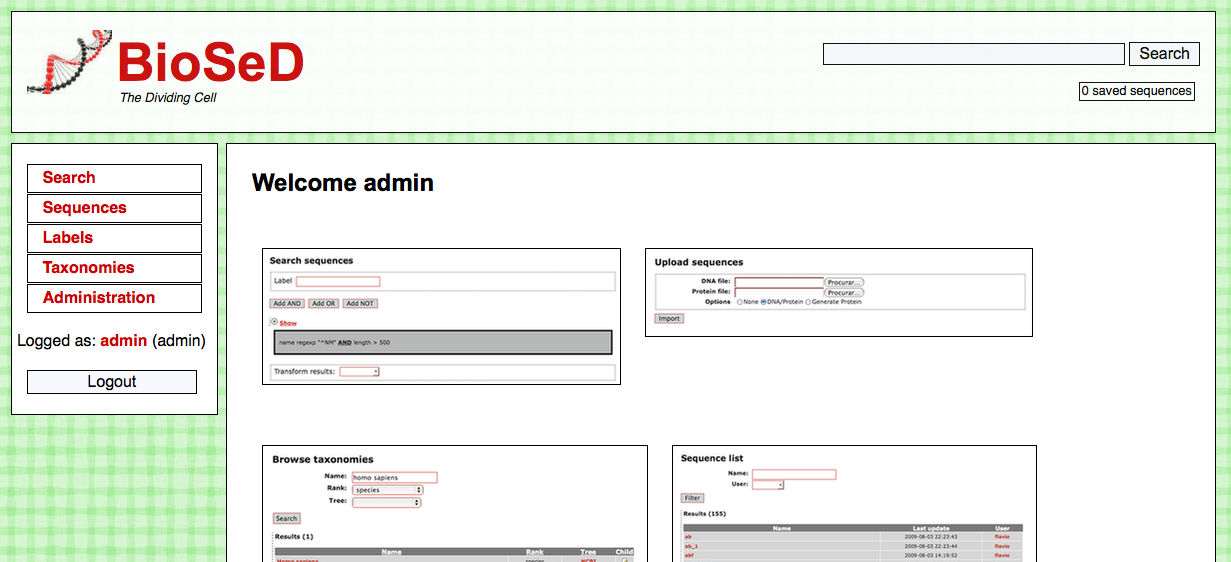
\includegraphics[scale=0.4]{interface.png}
  \caption{System home page.}
  \label{fig:home_page2}
\end{figure}

If you entered the correct password, the new page should look like Figure \ref{fig:home_page2}.

\section{Labels}

Label related options are found in the \textbf{Labels} submenu. For normal users
only the options \textbf{Labels - List} and \textbf{Labels - Export} are available.
The \textbf{admin} user has access to a few more options: \textbf{Labels - Add/New} and
\textbf{Labels - Import}.

\begin{figure}[H]
  \centering
    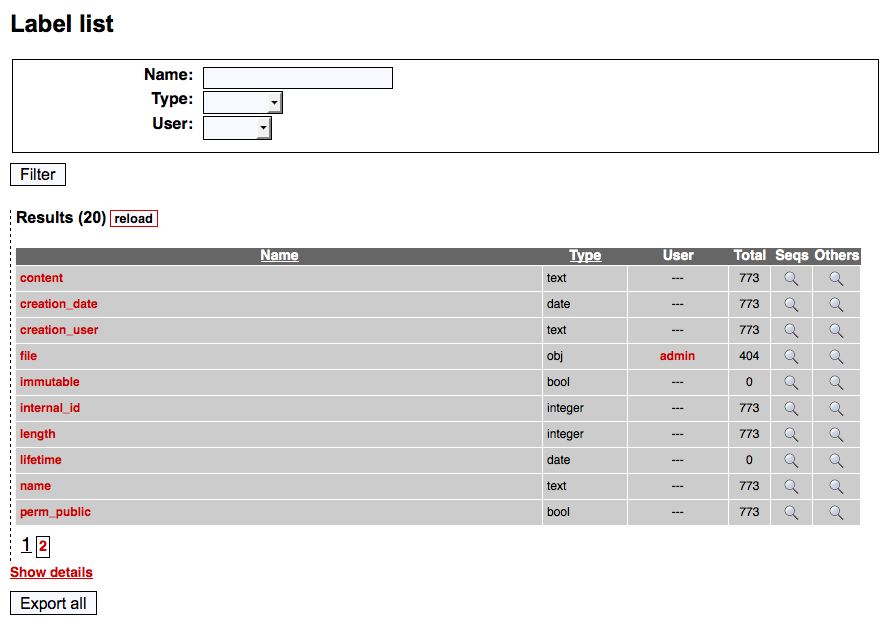
\includegraphics[scale=0.4]{label_list.png}
  \caption{Listing all labels}
  \label{fig:label_list}
\end{figure}

When listing labels, a page like Figure \ref{fig:label_list} should appear. The traditional
filter form is available and it is also possible to filter by label type.

The label types available are:
\begin{itemize}
  \item Integer: integer value.
  \item Float: float value.
  \item Text: text value.
  \item Position: pair of start and length values, representing a sequence's segment.
  \item Reference: pointer to another sequence.
  \item Taxonomy: pointer to a taxonomy.
  \item URL
  \item Bool: true/false value.
  \item Date: day, month and year triplet.
  \item Object: an uploaded file.
\end{itemize}

Still in this page, one can push the button \textbf{Export all} to export the current set of
labels being listed to XML. The button \textbf{Add new} redirects to the new label page, where one can
create a new label.

In the label list grid, special notes should be said about the columns:

\begin{itemize}
  \item Clicking on the label name redirects the application to the label's page.
  \item The column \textbf{Seqs} creates a new search page with sequences that contain that label.
  \item The column \textbf{Others} creates a new search page with sequences that do not contain that label.
\end{itemize}

\subsection{Creating new labels}

If you are an administrator, pushing the \textbf{Add new} button a new form will be presented.
The form contains all the fields needed to create a new label. They are:

\begin{itemize}
  \item \textbf{Name}: the label's name.
  \item \textbf{Type}: the label's type.
  \item \textbf{Code}: the code to generate a new label value using the sequence information as input.
  \item \textbf{Validation code}: code to validate a new label instance. Should return true if the value is valid, false otherwise.
  \item \textbf{Modification code}: block of code run after the sequence's content is updated. Should not return anything.
  \item \textbf{Comment}: comment about the label.
  \item \textbf{Must exist}: if true, every sequence must be annotated with this label, when that does not happen the label goes to the sequence's missing list.
  \item \textbf{Generate on creation}: if true when a sequence is created, the sequence will be automatically annotated with this label using the \textbf{Code} field.
  \item \textbf{Generate on modification}: if true and if the sequence is already annotated with this label, the label value is automatically changed using the \textbf{Code} field when the sequence's content is altered.
  \item \textbf{Deletable}: if true a specific label instance can be user deleted.
  \item \textbf{Editable}: if true a specific label instance can be user edited.
  \item \textbf{Default}: if true the label will me made system default and cannot be edited thereafter.
  \item \textbf{Public}: if true the label can be made part of public (no login) searches. 
\end{itemize}

All the code fields must be written in PHP \cite{php}.

Once created, you will be redirect to the label's page, where you can view or edit information about
the label. Each field can be changed by clicking on it.

Other options are present: \textbf{Delete} prompts you to delete the label, \textbf{Export} exports the label
to XML and \textbf{List labels} redirects you to the label list.

\subsection{Import / Export}

To export all labels you can use the option \textbf{Labels - Export} from the main menu. This
operation can be performed by any user.

Only the administrator is entitled to import files with labels. The option for this is
\textbf{Labels - Import}. There you should upload a XML file containing labels.
Once the file is processed a new report page is shown, as in Figure \ref{fig:import_labels}.

\begin{figure}[H]
  \centering
    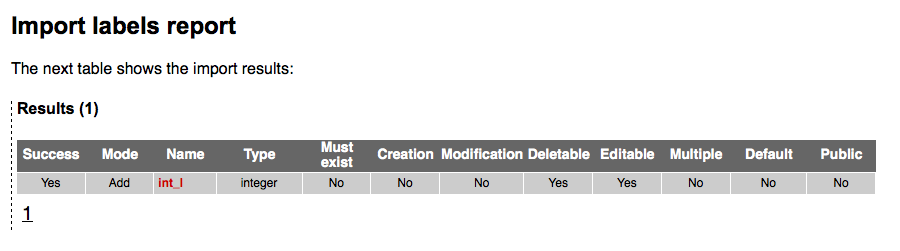
\includegraphics[scale=0.4]{import_labels.png}
  \caption{Import labels report}
  \label{fig:import_labels}
\end{figure}

The \textbf{Success} column tells if the label was successfully installed into the system
and the \textbf{Mode} column if the label is new to the system (mode \textit{add}) or the label
was already present and it was only updated (mode \textit{edit}).

\section{Sequences}

All sequence related options can be found in the \textbf{Sequences} submenu.
Three options can be found there: \textbf{List}, \textbf{Add/New} and \textbf{Batch}.

The \textbf{Sequences - List} option is used to list all system sequences. This page can also
be accessed without logging in, where only the labels annotated with the label \textbf{perm\_public}
as true will appear. This page also features a filter form.

More options are available in that page, namely:

\begin{itemize}
  \item \textbf{Search}: launches a new search page with the sequences present in the grid.
  
  \item \textbf{Add new}: redirects to a new page, where one can insert a new sequence.
\end{itemize}

To insert a new sequence one can use the \textbf{Add new} button or the \textbf{Sequences - Add/New}
option from the main menu. In the new sequence page, three fields are available: \textbf{Name}, for the
sequence name; \textbf{Content}, for the sequence content and \textbf{Generate protein}, that when the
sequence being insert is a DNA sequence, a protein sequence will be generated from it and the two sequences
will be automatically linked using the \textbf{translated} label.

Once the sequence is inserted, the user will be redirected to the sequence page (Figure \ref{fig:view_sequence}).
In this page, basic information about the sequence is shown, namely its name, content,
a link to the translated sequence, and, in the case of
sub-sequences, a link to the original sequence. In this page it is also possible to export the sequence,
by pushing the \textbf{Export} button.

The \textbf{Delete} button prompts you to delete the sequence and the \textbf{View labels} button
redirects you the sequence's label page.

\begin{figure}[H]
  \centering
    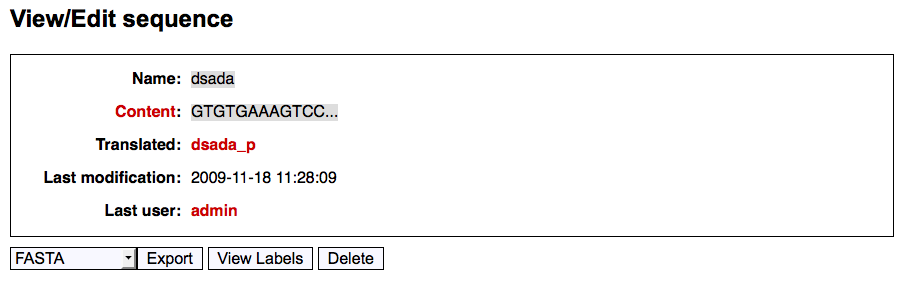
\includegraphics[scale=0.4]{view_sequence.png}
  \caption{Sequence page.}
  \label{fig:view_sequence}
\end{figure}

To edit sequence name or content just click in the respective name and content.

\subsection{Labels page}

Through the \textbf{View labels} button we can access the sequence's label page.

The labels page displays the sequence's annotated labels, labels available to add,
missing labels and non-multiple labels that have more than one instance for this sequence,
which we name the \textbf{bad multiple} labels.

The annotated labels list is always shown. The \textbf{Available} labels list
is only shown if the sequence is not annotated with every system label, which is the most frequent case.
The missing labels list is only shown if the sequence has not been annotated with
mandatory labels, like \textbf{type} or \textbf{length}. The bad multiple labels list
is only shown when, for some reason, the sequence is annotated with various instances of
the same label that is not multiple, this can happen when a label, once multiple, no longer is.

An example labels page in shown in Figure \ref{fig:labels2}. Some sets of labels are not shown
by default and must be displayed by clicking \textbf{Show}. Filtering of labels is also available
as shown in the example page.

\begin{figure}[ht]
  \centering
    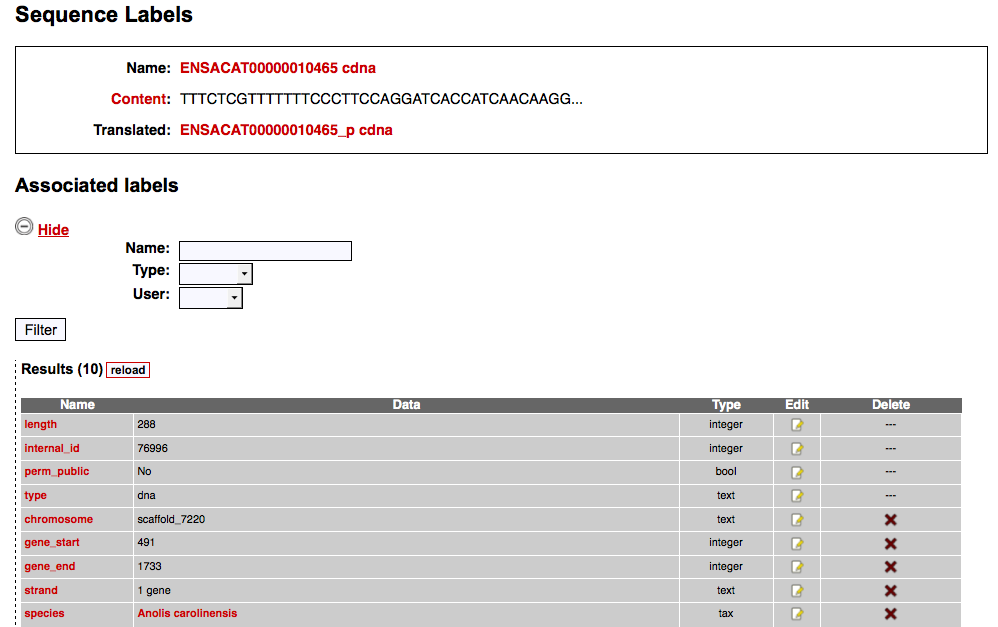
\includegraphics[scale=0.5]{labels.png}
  \caption{Example labels page.}
  \label{fig:labels2}
\end{figure}

Some useful interactions were implemented: clicking in one missing label opens the available pages
separator and highlights the label there, easing the process of annotating the sequence with missing
labels; clicking in one bad-multiple label highlights the specific label instance in the annotated labels list.

Clicking on the \textbf{Show details} link forces the annotated labels list to display more details
about the labels.

Multiple labels are shown as \textit{label\_name[parameter]}, where \textit{parameter} is the multiple
label parameter.

Clicking \textbf{Add} the icon from the first column of the \textbf{Available labels} list popups a new window
that will be used to create a new label instance. To delete any annotated label,
just use the icons from the \textbf{Delete} column
from the same list. The \textbf{Data} column displays the label value and for label types like
reference, object, taxonomy or URL, a link is rendered that redirects you to the resource.

The \textbf{Edit} icon from the annotated labels list
launches a new window to edit the current label value.
This window is similar to the one used to insert new label instances.

The edit or add label popup windows display forms where the user can insert or edit label values.

If the label supports automatic generation a checkbox \textbf{Generate default value} is displayed.
If checked in, the result will be a new label instance generated from the label code.

For each label type, the popup window is slightly different. Next's a summary is enumerated:

\begin{itemize}
  \item \textbf{integer}, \textbf{float}: text field with numeric validation.
  \item \textbf{text}: simple text field.
  \item \textbf{url}: text field with URL validation.
  \item \textbf{bool}: a checkbox.
  \item \textbf{position}: two text fields with numeric validation.
  \item \textbf{taxonomy}: a searchable grid with taxonomies that can be selected.
  \item \textbf{reference}: a searchable grid with sequences that can be selected.
  \item \textbf{date}: text field with calendar widget.
  \item \textbf{object} (Figure \ref{fig:obj_label2}): if the label has files attached a select list is displayed containing them.
  An upload field is also available.
\end{itemize}

\begin{figure}[ht]
  \centering
    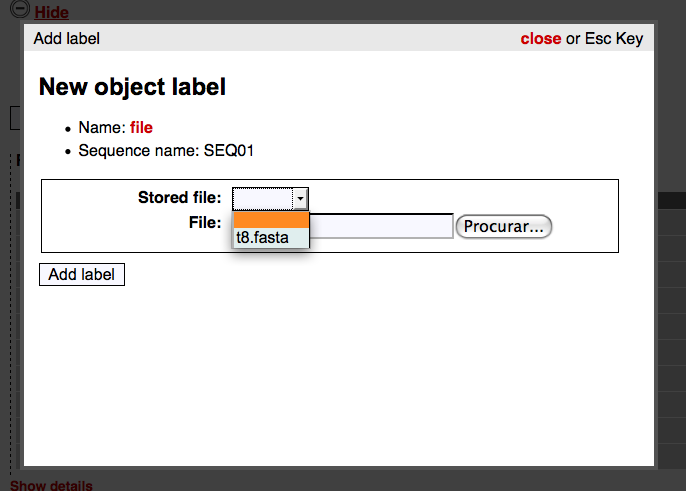
\includegraphics[scale=0.5]{obj_label.png}
  \caption{Annotating a new object label.}
  \label{fig:obj_label2}
\end{figure}

Once a label instance is added or edited the labels page is updated to reflect the changes.

\subsection{Batch}

Instead of inserting sequences one by one using the page described above, you can
upload a file with several sequences in either XML or FASTA format. These files
can be also annotated with labels as described in the section \ref{sec:file_formats}.

When uploading the file, the system will try to insert or update the stored sequences.
A sequence is only updated if the application can found a previously stored sequence with
the same name and content, everything else is treated as a new sequence.

To access this functionality use the \textbf{Sequences - Batch} main menu option.

In this page (Figure \ref{fig:sequence_upload2}) three options are available: upload a single file; upload both DNA and protein file, linking
the sequences along the process; upload a DNA file and also generate protein sequences.
When converting DNA to protein sequences, it is possible to annotate the protein sequences
with the same DNA labels by using the \textbf{Keep structure} option.

\begin{figure}[ht]
  \centering
    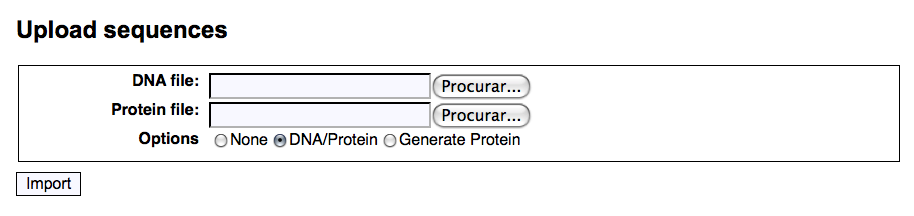
\includegraphics[scale=0.5]{sequence_upload.png}
  \caption{Upload sequences page.}
  \label{fig:sequence_upload2}
\end{figure}

When the file is being processed a loading screen appears displaying the progress.
When everything is done a report page like the Figure \ref{fig:batch_report2} should appear.

\begin{figure}[ht]
  \centering
    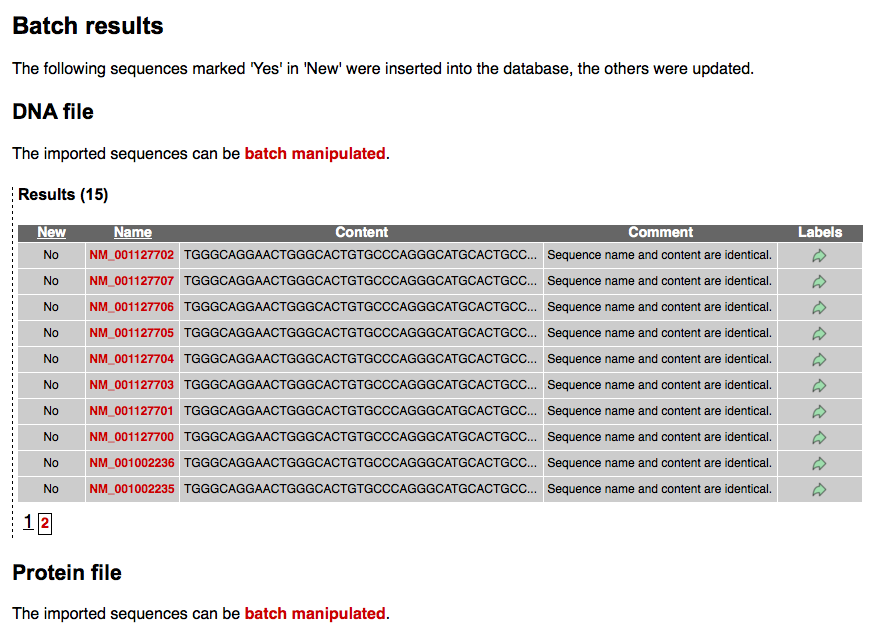
\includegraphics[scale=0.5]{batch_report2.png}
  \caption{Batch sequence report.}
  \label{fig:batch_report2}
\end{figure}

If the \textbf{none} option was chosen, only a list of sequences is shown, for everything else,
a list of DNA and protein sequences are shown.

If the files sent were annotated with labels, a label report is shown, indicating the state for each label.
For example, if a label present in the file is not installed in the system, a warning indicating the label
is not installed will be shown. Only previously installed labels will be used when importing label values.

In each sequence list the \textbf{New} column indicates if the sequence is new and was inserted, or if it is old
and it is being updated. The \textbf{Comment} label displays various kinds of informations and can tell when
the sequence was only updated.

If the file was annotated with labels, a column named \textbf{Status} will appear in the sequence list. Clicking
on the green arrow will popup a window with a grid, indicating for each label, the status for this sequence.
For example, if a label is automatically generated when a sequence is created and its value was specified in the file,
the label will not be updated and the text \textbf{Already inserted} will be shown.

Clicking on the \textbf{batch manipulated} link will redirect you to a new search page with only the imported sequences,
which is useful to run various operations for all those sequences in batch mode.

\section{Taxonomies}

To manage taxonomies we should pay attention to three things: trees, taxonomy ranks and taxonomies.

With taxonomy trees one can have multiple trees of taxonomies, which is useful to have custom
taxonomies and more scientific trees like the NCBI taxonomy tree.

Ranks is one way to categorize taxonomies. The system installs a rich set of ranks,
with parent/child relationships already defined.

To access taxonomy related features, use the \textbf{Taxonomies} submenu from the main menu.

\subsection{Managing trees}

To list the currently defined taxonomy trees, select \textbf{Taxonomies - Trees - List}, there
you should at least see the NCBI tree (Figure \ref{fig:tree_list}).

\begin{figure}[H]
  \centering
    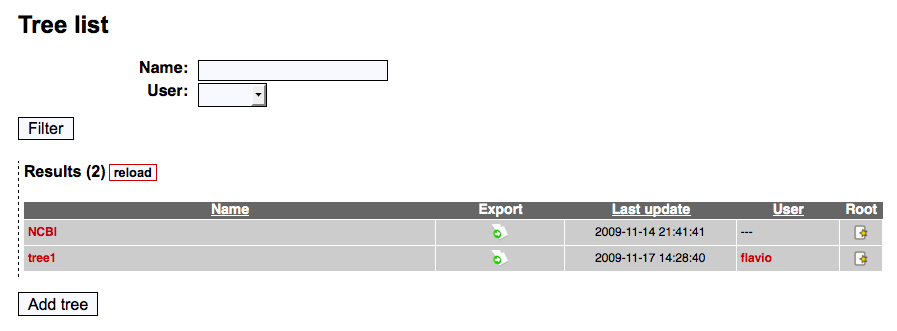
\includegraphics[scale=0.4]{tree_list.png}
  \caption{Tree listing.}
  \label{fig:tree_list}
\end{figure}

The user has the possibility to filter the tree list using a tree name or the user who made the last update.

From here you can select a tree to view or edit or select \textbf{Add tree} to create a new tree.
To create a new tree you can also use \textbf{Taxonomies - Trees - Add/New}.

Each tree can also be exported to a XML file using the green \textbf{Export} button.
The yellow \textbf{Root} button helps creating a new root taxonomy for this tree.

Selecting \textbf{Add tree}, you will be prompted for the tree name. Once created, you will be
redirected to the tree's page, as in Figure \ref{fig:view_tree}.

In it you can see history information and also edit the tree name by clicking on it.

There is also four operation buttons:

\begin{itemize}
  \item List trees: redirects you back to the tree list.
  \item Export: exports the tree to a XML file.
  \item Delete: prompts you to delete the tree (not available for the NCBI tree).
  \item Browse: enables you to browse the tree.
\end{itemize}

\begin{figure}[H]
  \centering
    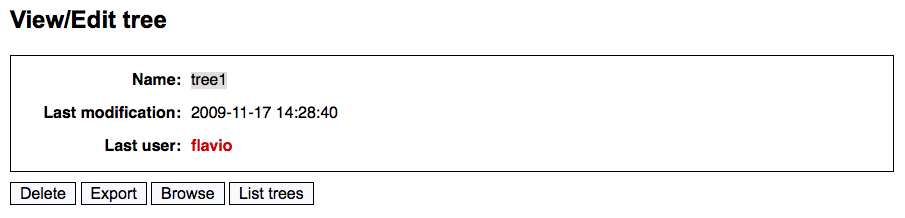
\includegraphics[scale=0.4]{view_tree.png}
  \caption{Viewing a tree.}
  \label{fig:view_tree}
\end{figure}

If you are an administrator you can make use of the option \textbf{Taxonomies - Trees - Import}
to upload a taxonomy tree XML file. Once the file is uploaded, the system tries to insert
all taxonomies from that tree into the system. If some taxonomies are found, updates are done.

\subsubsection{Tree browsing}

The tree browser page provides an easy to use interface to navigate through the target tree.

In Figure \ref{fig:tree_browsing} we are navigating the NCBI tree, currently at node \textbf{root}
and the grid is filled with \textbf{root}'s children.

We can go up in the hierarchy by clicking \textbf{Go up \textit{node name}}. To navigate into
a taxonomy we click the green arrow in the select column for that taxonomy. We can also
add a new taxonomy child, selecting the last icon from the \textbf{Child} column, it redirects us
to a new taxonomy form, with the parent taxonomy already setup.

\begin{figure}[H]
  \centering
    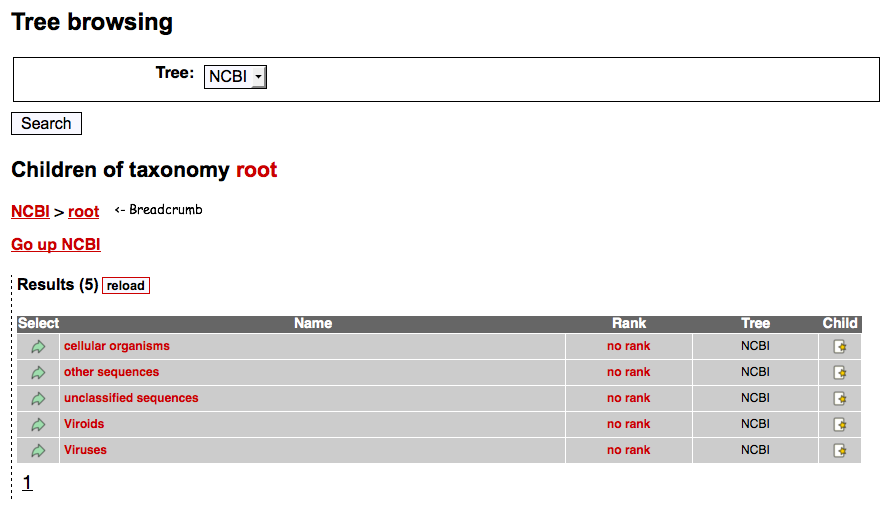
\includegraphics[scale=0.4]{tree_browsing.png}
  \caption{Browsing the NCBI tree.}
  \label{fig:tree_browsing}
\end{figure}

Another important aspect is the breadcrumb component (in the example \textbf{NCBI $>$ root}). Clicking
in one breadcrumb name will make the current taxonomy change.

\subsection{Managing ranks}

To list all system ranks use the option \textbf{Taxonomies - Ranks - List} from the main menu.
This page gives you a filter enabled rank list, being possible to filter the rank list by
rank name, parent rank name or the user who made the last rank change.

You can also order the rank names by alphabetical order, ascending or descending.

To export the current set of ranks just push the \textbf{Export all} button.

For each rank in the grid, there are two action icons: one named \textbf{Taxonomy}, that redirects us
to the new taxonomy form where the rank is already selected, and the other, \textbf{Child}
opens a new page with a form to create a new rank with the parent rank already set.

To create ranks, there's also the \textbf{Taxonomies - Ranks - Add/New} menu option.
On this page, you should input the rank name and select the parent rank from the list of inserted ranks.

Once a rank is created, the system redirects you to the rank page where you can edit the rank name
or parent rank by clicking in the respective name. Editing by clicking on the name, changes the rank name
to a text field, where you can input the new name and then, when pushing the \textbf{OK} button, sends the
changes back to the server.

Also, when on the rank page, there are two buttons at the end of the page: \textbf{Delete} prompts you to
delete the rank and \textbf{List ranks} redirects you back to the rank list.

\subsubsection{Import / Export}

When logged in as \textbf{admin} you can export all system ranks through the option
\textbf{Taxonomies - Ranks - Export}. The output file is XML.

The other way around, you can import a XML file with ranks, through the option
\textbf{Taxonomies - Ranks - Import}. Once the file is processed by the server
a page like Figure \ref{fig:rank_import} is shown.

The column \textbf{Success} tells if the new rank was installed into the system or not,
the column \textbf{Mode} indicates if the new rank was added or edited. The \textbf{Parent found}
column tells if the parent was found in the system (if the system can not find it, it is created).
The column \textbf{Original parent} was the rank parent before the import operation if the rank
was already in the system and the column \textbf{Parent} just indicates the new parent rank.

\begin{figure}[H]
  \centering
    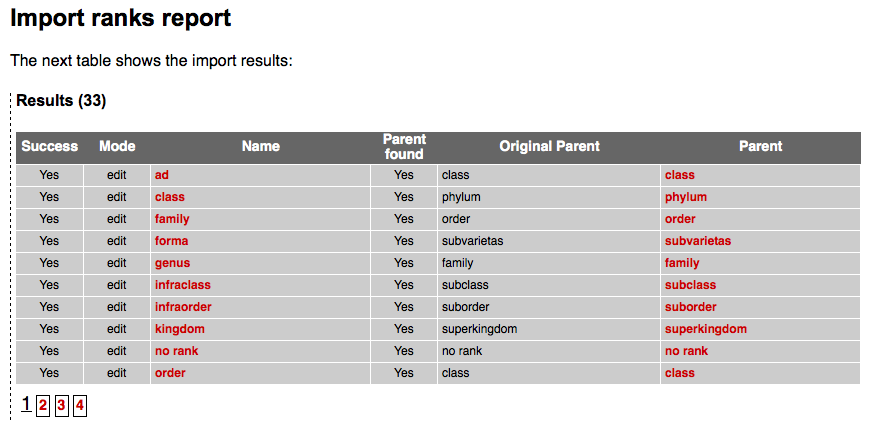
\includegraphics[scale=0.4]{rank_import.png}
  \caption{Import rank report}
  \label{fig:rank_import}
\end{figure}

\subsection{Managing taxonomies}

We have seen that there are lots of ways to get to the new taxonomy form. The standard way is to
choose the option \textbf{Taxonomies - Add/New} from the main menu. There you should enter the
taxonomy name, choose the rank and tree from a list of stored ranks and trees, respectively.

The rank and tree can be left empty, but as a recommendation, you should define them right
from the beginning.

Once a taxonomy is created, the system redirects you to the taxonomy page.
Each taxonomy page is composed of: a form where you can edit basic taxonomy information (Figure \ref{fig:taxonomy_basic}),
a list of optional taxonomy names (Figure \ref{fig:other_names}) and a list of children taxonomies.

In the first part (Figure \ref{fig:taxonomy_basic}), you can edit the name and rank by clicking in the respective name.
Changing the tree is not allowed. To change the parent you should click the red \textbf{Parent:} link and when
a window popup appears you should search for your parent taxonomy, select the name from the grid and then push
the \textbf{Select} button.

\begin{figure}[H]
  \centering
    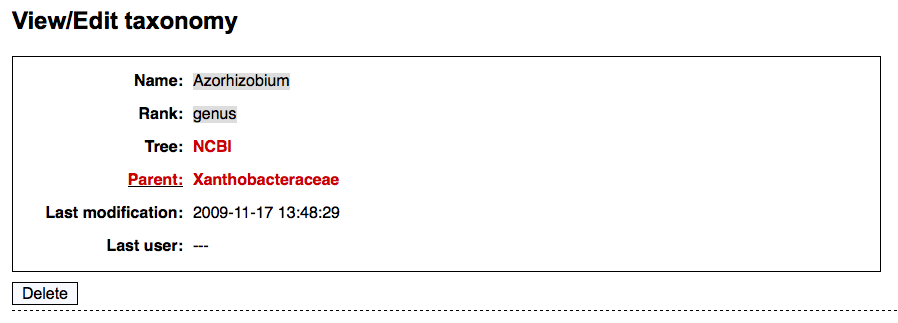
\includegraphics[scale=0.4]{taxonomy_basic.png}
  \caption{Editing taxonomy information.}
  \label{fig:taxonomy_basic}
\end{figure}

The \textbf{Other names} section provide a list of other names for the taxonomy. Each name can be deleted
using the \textbf{Delete} column. To edit a name you should click on the name cell and then push the \textbf{OK}
button. To edit the name type the process is identical. To add a name, just use the provided form.

\begin{figure}[H]
  \centering
    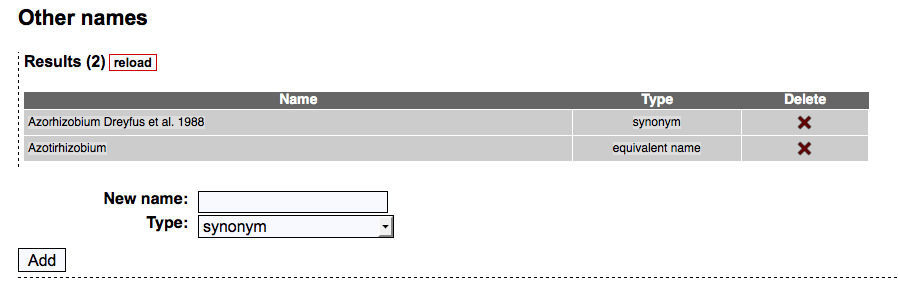
\includegraphics[scale=0.4]{other_names.png}
  \caption{Other names section.}
  \label{fig:other_names}
\end{figure}

The final section displays a grid with the children taxonomy. You can add new ones to the list by pushing
the \textbf{Add child} button.

As the number of taxonomies can get very large, we provided a page where one can search by taxonomies
by just using the name, tree or rank, or any combination of these.

To use this interface go to \textbf{Taxonomies - Browse}.

\section{Search}

To search sequences using the annotated label information, one can use the search pages available
from the main menu. Three pages are available:

\begin{itemize}
  \item \textbf{Search - ALL}: to search all sequences.
  \item \textbf{Search - DNA}: search only DNA sequences.
  \item \textbf{Search - Protein}: search only protein sequences.
\end{itemize}

All the three search pages look the same, so everything we will describe for the rest
of this section will apply for all of them.

Accessing any search page, we will rapidly discover three main sections in this page:
the query input section, the operations section and the preview section.

\subsection{Query input}

The query input section (as shown in Figure \ref{fig:search1_man}) presents you controls
to display and manipulate the query expression.

The query is presented in two formats: the tree, where you can manipulate parts of the expression
and the query text, where the query is presented in an human readable format. In the query tree view,
apart from selecting where to insert sub-expressions, you can also delete parts of the expression by
selecting an AND, OR, NOT or terminal expression and pressing \textbf{Delete}.

To insert a new query expression, you should choose where the expression will be put. That is possible
selecting one of the previously inserted OR, AND or NOT expressions. If you simply want
to create a simple AND query expression, press the \textbf{Reset} button and start
inserting expressions. But if you want to create complex queries you should know how to
insert expressions at different positions.

\begin{figure}[H]
  \centering
    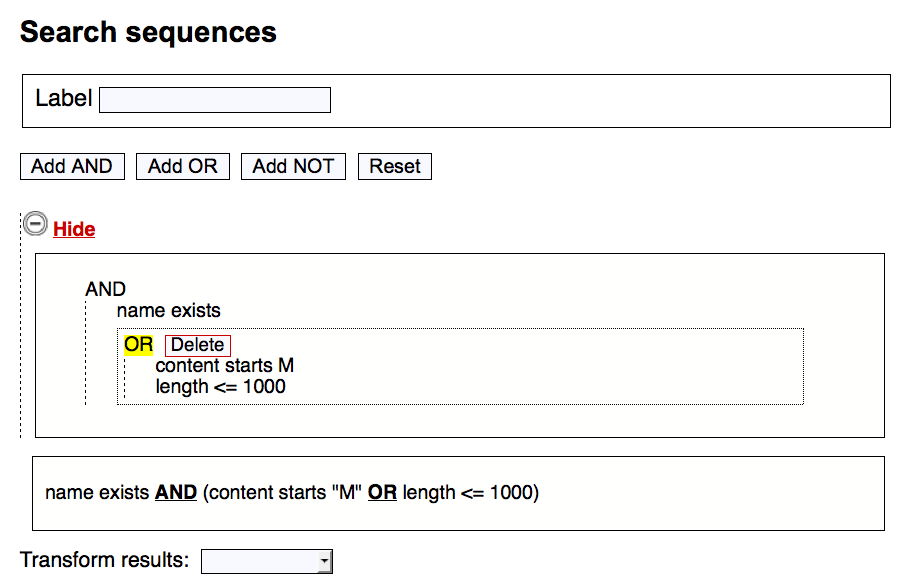
\includegraphics[scale=0.5]{search1.png}
  \caption{Search query input.}
  \label{fig:search1_man}
\end{figure}

When creating a new sub-expression, the process involves various steps:

\begin{itemize}
  \item First, input the label name you want to use for this term in the \textbf{Label} field.
  The system will autocomplete the label names as you type.
  \item When a label is chosen, you must select the search operator. Please see the table \ref{tbl:operators}
  for information about each operator.
  \item After the operator is chosen, you must, optionally, input the value for the operator.

  In resume, for each label type:
  
  \begin{itemize}
     \item Text, URL and Object: Text field.
     \item Integer, position and float: Numeric text field.
     \item Bool: Checkbox.
     \item Date: The date is input in a calendar widget. Please click on the text field to activate it.
     \item Taxonomy: Text field for the \textbf{like} operator. For the \textbf{equal} operator you should
      click on the \textbf{Find taxonomy} link, search a taxonomy within the popup window and then click on
      the chosen taxonomy name.
     \item Reference: Text field for the \textbf{like} operator. For the \textbf{equal} operator you should
      click on the \textbf{Find sequence} link, search a sequence within the popup window and then click on
      the chosen sequence.
  \end{itemize}

  \item Press the \textbf{Add term} button. The new term should appear on the query views, and the preview
  section will be automatically updated.
\end{itemize}

Please remember that you can use the \textbf{exists} and \textbf{not exists} operators. These
operators will filter sequences that are annotated with a label or not, respectively, and do not need
values.

If the label is multiple, you can, optionally, input the multiple parameter. If the multiple parameter is
not given, the search is done for all label instances. If given, the query will only use the specific label instance.

You can also insert AND, OR and NOT terms. Use the respective buttons.

\begin{table}[H]
  \scalebox{0.7}{%
    \begin{tabular}{ | c | p{1.2\textwidth} |}
      \hline
      \textbf{Label type} & \textbf{Operators} \\ \hline
      
      URL, text and object & \begin{itemize}
        \item equal: Equal comparison.
        \item contains: If the label contains a substring.
        \item starts: If the instance starts with.
        \item ends: Starts counterpart.
        \item regexp: Regular expression matching.
      \end{itemize} \\ \hline
      
      Bool & \begin{itemize}
        \item equal: Equal comparison.
      \end{itemize} \\ \hline
      
      Integer and float & \begin{itemize}
        \item $=$
        \item $>$
        \item $<$
        \item $>=$
        \item $<=$
      \end{itemize} \\ \hline
      
      Position & \begin{itemize}
        \item $=$
        \item $>$
        \item $<$
        \item $>=$
        \item $<=$
      \end{itemize} You should also select the position component, start or length for the term.
      \\ \hline
      
      Date & \begin{itemize}
        \item equal: Equal comparison.
        \item before: Date is before some date.
        \item after: Date is after some date.
      \end{itemize} \\ \hline
      
      Taxonomy & \begin{itemize}
        \item equal: Equal comparison.
        \item like: A taxonomy name to search for. Using this operator will make system search for all
        taxonomies in the database with this name and then the query will match if a sequence points to any of them.
      \end{itemize} \\ \hline
      
      Reference & \begin{itemize}
        \item equal: Equal comparison.
        \item like: A sequence name to search for. Works the same way as for taxonomies.
      \end{itemize} \\ \hline
  \end{tabular}}
  \caption{Label types and operators.}
  \label{tbl:operators}
\end{table}

One important option in this section is \textbf{Transform results}. Here you can select a reference label,
and the results will be transformed using the annotated reference label in each sequence.
If not all sequences are annotated with that label, the new result set will be smaller than the original.
If the reference label is multiple, the new result set can be potentially bigger.

Please note that the new, transformed, set will be used for the following operations.

\subsection{Operations}

While you create your complex query you can see the preview component getting refreshed,
with either the result total, or, optionally, the result list. Finally, once the query is built,
you can do operations on the results.

The operations section as it can be seen in Figure \ref{fig:search2_man}, contains various operations
you can do to the search result list.

\begin{figure}[H]
  \centering
    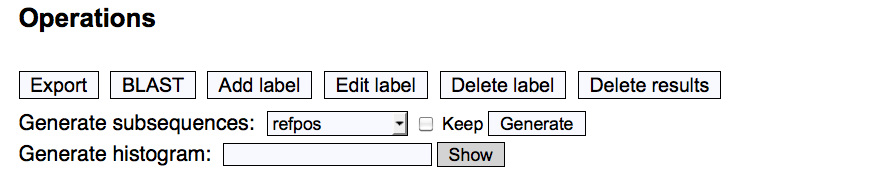
\includegraphics[scale=0.5]{search2.png}
  \caption{Search operations.}
  \label{fig:search2_man}
\end{figure}

\subsection{Sub-sequences}

We can generate sub-sequences using a position label from the result list. For example,
if your sequences contain a position label for a specific sequence segment, you can generate
sub-sequences for the complete set of sequences. To do that, you must select the position label
from the \textbf{Generate subsequences} select list and then push the \textbf{Generate button}.
If you want to keep your sub-sequences around longer than a few days, you should check the \textbf{Keep}
checkbox. When not keeping the sequences around, the system will delete them after some hours.

Once the sub-sequences are generated, a report page will be shown.

\subsection{BLAST}

The BLAST search option is used to do a BLAST search
over the result sequence list using an arbitrary number of 
query sequences.

The BLAST page is displayed on Figure \ref{fig:blast2} and shows two distinct
sections: section (1) for basic BLAST setup, section (2) for advanced parametrization.

\begin{figure}[ht]
  \centering
    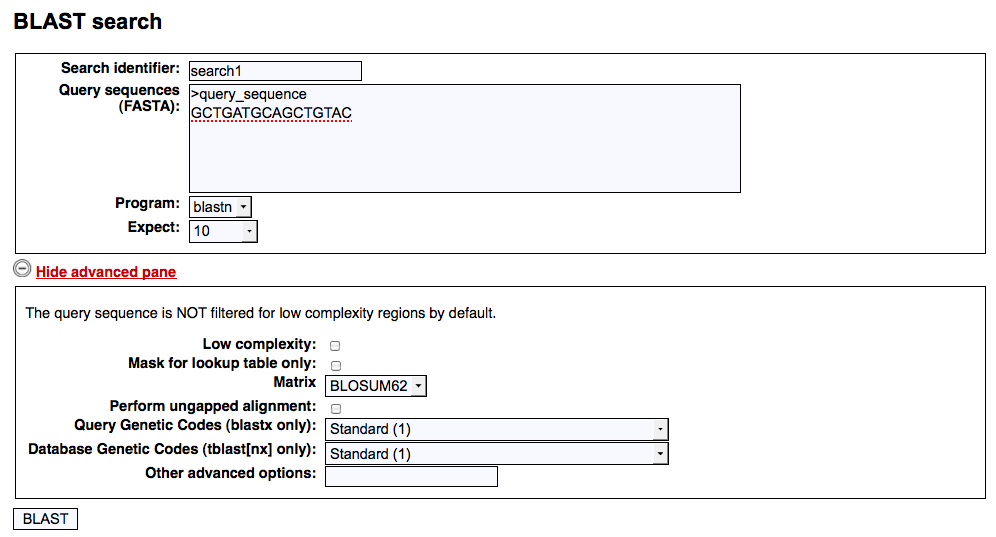
\includegraphics[scale=0.45]{blast.png}
  \caption{BLAST search screen.}
  \label{fig:blast2}
\end{figure}

In the first section, a search identifier must be provided, which identifies
this specific search and the query sequences in FASTA format that will be
matched against the result sequence list. It is also possible to
select between specialized BLAST programs, depending on the result sequence list
characteristics, but usually this option is pretty restricted by the system knowledge of
the sequences. Finally, the default \textit{expect} value can be changed to best
suit the search purposes.

The second section provides more advanced BLAST options.
If some BLAST option can not be found, the \textbf{Other advanced options} input box
is provided to pass arbitrary \texttt{blastall} program arguments.

Once the BLAST parameters are set, the \textbf{BLAST} button launches the BLAST
search and a new page is loaded (Figure \ref{fig:blast_results2}), presenting the BLAST output and a button to,
optionally, annotate each matched sequence with BLAST information.

\begin{figure}[ht]
  \centering
    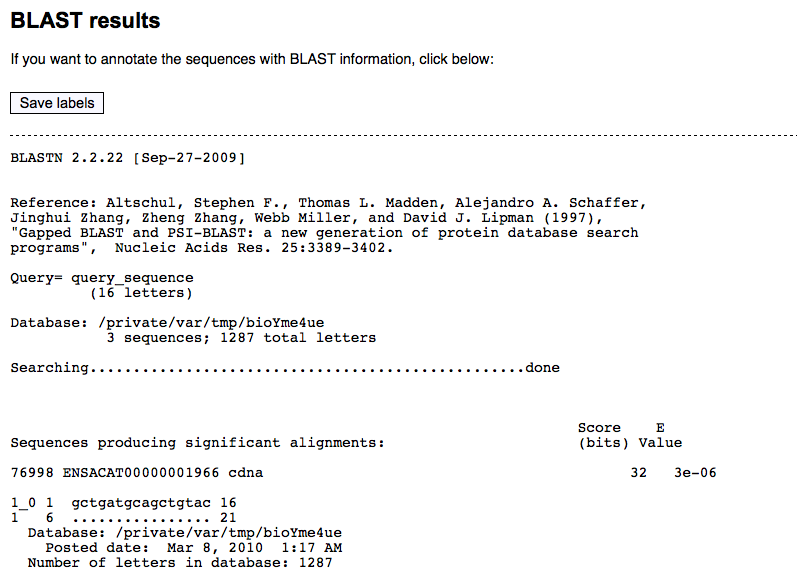
\includegraphics[scale=0.45]{blast_results.png}
  \caption{BLAST results screen.}
  \label{fig:blast_results2}
\end{figure}

The following labels are used:

\begin{itemize}
  \item \textbf{evalue} (float): Expectation value.
  \item \textbf{blast\_score} (float): BLAST score.
  \item \textbf{blast\_query} (boolean): True if the sequence matched the BLAST search.
\end{itemize}

Each one of these labels can have multiple instances and is parametrized by a search identifier
and the name of the matched query sequence.

For example, the search identifier provided was \textit{search1}, the
query sequences only included one sequence named \textit{query\_sequence} and
one sequence on the result list matched the query sequence.
The following annotations would be made:

\begin{itemize}
  \item \texttt{evalue[search1:query\_sequence] = 3e-06}
  \item \texttt{blast\_score[search1:query\_sequence] = 32}
  \item \texttt{blast\_query[search1:query\_sequence] = Yes}
\end{itemize}

\subsection{Histograms}

Another operation is the \textbf{Generate histogram} (Figure \ref{fig:histogram_man}).
This option can generate an histogram
for that label distribution across the result list. For example, you could generate a length
distribution for a given sequence set and then the system will generate the frequency histogram
and display the distribution total and number of classes.
For numeric labels the smallest class, largest class, average, median and mode values are also shown.

If your label is multiple and numeric, you can chose what value will be representative for each sequence.
You can use the average value for all label instances from a sequence, the minimum or the maximum value.
If the label is not numeric but multiple, all values will be considered.

\begin{figure}[ht]
  \centering
    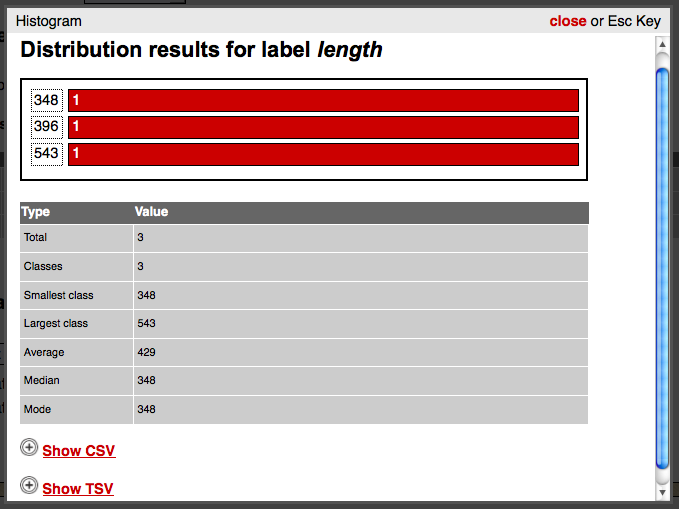
\includegraphics[scale=0.4]{histogram.png}
  \caption{Plotting histograms.}
  \label{fig:histogram_man}
\end{figure}

In the popup window that appears when generating the histogram, you can also copy the distribution values
to use with programs like Microsoft Excel.

\subsection{Export}

Another important operation is the \textbf{Export} button.
It can export your result sequences (Figure \ref{fig:export_search})
into the file formats mentioned before and supported by the system.

For formats like FASTA, CSV or XML, you can select the labels that will appear on the file, only exporting annotation 
that is important to the task at hand.

\begin{figure}[ht]
  \centering
    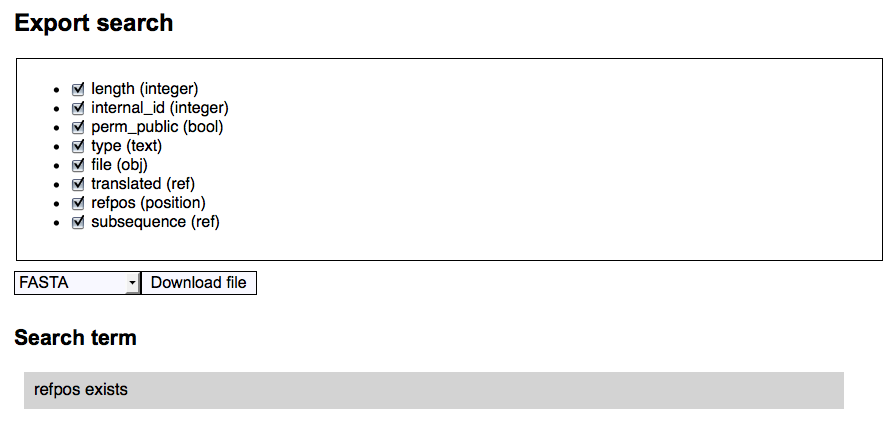
\includegraphics[scale=0.4]{export_search.png}
  \caption{Export search page.}
  \label{fig:export_search}
\end{figure}

\subsection{Batch labels}

Another common action to do is, for example, annotate a list of sequences with the same label instance.
For this you can use the button \textbf{Add label}, to add, or the button \textbf{Edit label}, to edit.

Using the \textbf{Add label} option you will be redirected to a page that looks like Figure \ref{fig:add_label_batch}.
First you should enter the label name into the \textbf{Label} text field, optionally you can check the \textbf{Update}
checkbox. When checked and if the sequence already contains that label instance, the current value will updated; if not
checked, nothing will be done.

When ready press the \textbf{Next...} button. A popup window should appear.
This window is very similar to the one we used to add a label to a sequence, so, it works the same way.

Once you input the label value, a report on the process should appear, right below the \textbf{Next...} button.

\begin{figure}[ht]
  \centering
    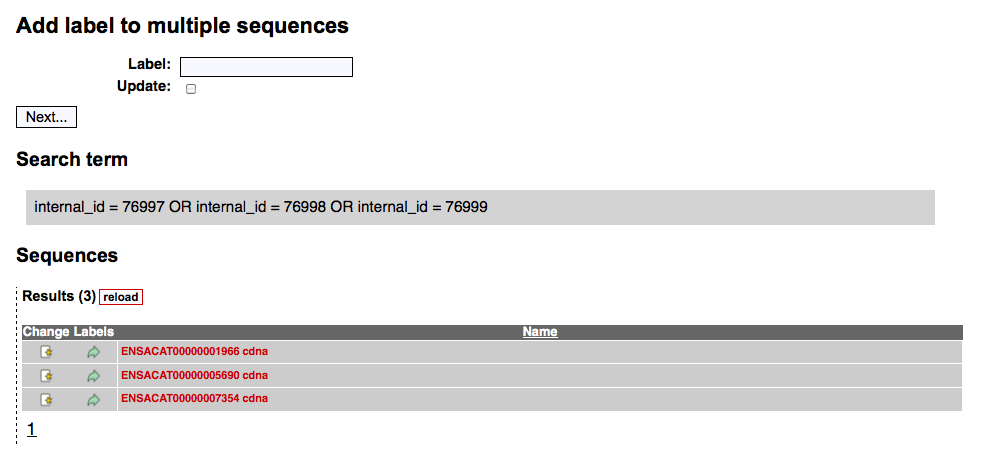
\includegraphics[scale=0.4]{add_label_batch.png}
  \caption{Add label to multiple sequences.}
  \label{fig:add_label_batch}
\end{figure}

The \textbf{Edit label} operation works in a similar fashion, but instead of having the \textbf{Update} checkbox,
it contains the \textbf{Add new} checkbox. This checkbox, when checked and when the sequence does not contain the
label, forces the system to add a new label value. It is the counterpart of the \textbf{Update} option, but for
the designed for the edit mode.

There is still another button, the \textbf{Delete label} button. This button gives you the possibility
to delete a label from the set of sequences. After you put the label, press the \textbf{Next...} button and
answer \textbf{Yes} and all annotations related to that label will disappear from the sequence list.

\subsection{Delete}

If you want to delete your sequence list just select the button \textbf{Delete} and
everything will be deleted. The action is irreversible, so use it with care!

\subsection{Preview}

The middle section (Figure \ref{fig:search3_man}) present in the search page is the preview section. In it
we can see the results for the query being build, as either the final total or the result list in a data grid.

\begin{figure}[H]
  \centering
    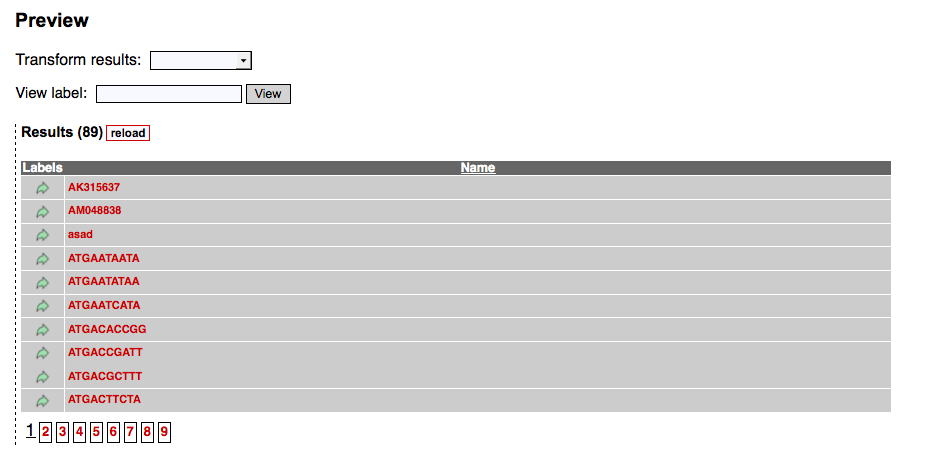
\includegraphics[scale=0.5]{search3.png}
  \caption{Search preview results.}
  \label{fig:search3_man}
\end{figure}

The \textbf{View label} option, can add new label columns to the result grid, showing the label
values for each sequence, as shown in Figure \ref{fig:view_label}.

\begin{figure}[H]
  \centering
    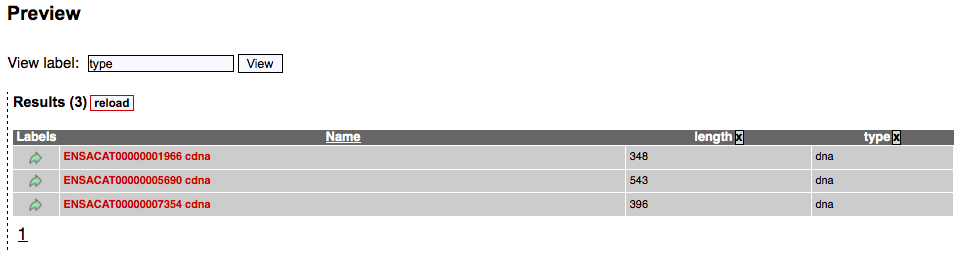
\includegraphics[scale=0.5]{view_label.png}
  \caption{Using view label.}
  \label{fig:view_label}
\end{figure}

Each new label column added can be removed by clicking the \textbf{X} on the column header.

\subsection{Written queries}

Instead of using the query input section from the search page, you can use the search field
on the top of each page to input arbitrarily complex queries.

The search field can also search for anything in the system: labels, taxonomies, ranks and sequences.
When the specified search expression is not valid, the system will fallback to a wide search for the
former objects, displaying a page with a grid for each entity where the query matched. So, for example,
if you input 'homo sapiens', the system will display a grid with taxonomies with 'homo sapiens' in the name.

But the more interesting case is when using valid query expressions. A query expression
is composed of terminal expressions and composed expressions.

A terminal expression contains a label name, an operator and, optionally, a value.
The following expression is a terminal expression: \textit{length $>$ 500}. The operators that
do not need a value, are the \textbf{exists} and \textbf{notexists} operators, like \textit{species exists}.
For everything else the form is \textit{label\_name operator value}. Operators and value information
is shown in table \ref{tbl:operators_values_expressions}.

Another note: if you want to write values with spaces, wrap the value around ' or ".

\begin{table}[ht]
  \scalebox{0.75}{%
    \begin{tabular}{ | c | p{0.4\textwidth} | p{0.7\textwidth} |}
      \hline
      \textbf{Label type} & \textbf{Operators} & \textbf{Values} \\ \hline
      
      URL, text and object & \begin{itemize}
        \item equal: Equal comparison.
        \item contains: If the label contains a substring.
        \item starts: If the instance starts with.
        \item ends: Starts counterpart.
        \item regexp: Regular expression matching.
      \end{itemize} & --- \\ \hline
      
      Bool & \begin{itemize}
        \item equal: Equal comparison.
      \end{itemize} & The value should be "true" or "false". \\ \hline
      
      Integer and float & \begin{itemize}
        \item $=$
        \item $>$
        \item $<$
        \item $>=$
        \item $<=$
      \end{itemize} & The value should be a number. \\ \hline
      
      Position & \begin{itemize}
        \item $=$
        \item $>$
        \item $<$
        \item $>=$
        \item $<=$
      \end{itemize} & Before the operator you should indicate the position component to compare: 'start' or 'length'. \\ \hline
      
      Date & \begin{itemize}
        \item equal: Equal comparison.
        \item before: Date is before some date.
        \item after: Date is after some date.
      \end{itemize} & Values should be in the form \textit{dd-mm-yyyy} like \textit{03-11-2009}. \\ \hline
      
      Taxonomy & \begin{itemize}
        \item like: A taxonomy name to search for.
      \end{itemize} & The \textbf{like} operator gets a taxonomy name and then searches all taxonomies
      with that name in the system and if the sequence points to any of them the query succeeds. \\ \hline
      
      Reference & \begin{itemize}
        \item like: A sequence name to search for.
      \end{itemize} & The values and operators work just like the taxonomy labels, but applied for sequences. \\ \hline
  \end{tabular}}
  \caption{Operators and values in query expressions.}
  \label{tbl:operators_values_expressions}
\end{table}

Now, composed expressions can combine various other expressions, recursively, and use the special operators: AND, OR or NOT.
AND and OR can be used like \textit{expression1 AND expression2 AND expression3 ...}. The NOT operator can only have
an expression as argument, like this: \textit{NOT expression}.

You can also use parenthesis to group expressions. So for example, you can have things like:
$<$\textit{(length $>$ 500 and name exists) or content regexp AGTG}$>$.

Once you input the expression, the system will analyze it and build a tree for it, redirecting you to the search page,
where you can run batch operations against the resulting sequences.

\section{File formats}

For file format information please read the section \ref{sec:file_formats} from the main technical report.

\section{Administration}

There are a few functionalities to do maintenance or administration tasks.
These tasks can only be used when logged in as \textbf{admin}.

\subsection{User management}

One of the key areas in administration is user management.
Lets see how we can add new users, update user settings and so forth.

\subsubsection{New user}

To create a new user select \textbf{Administration - Users - Register} and input the user information.
The username field is the name that should be used to login. You must also input the
user's password twice. Click \textbf{Do register}. If everything went well,
a new user has been registered and a list of all system users is shown.

This list can be accessed through \textbf{Administration - Users - List}.

Create more users as needed. You can also logout and try the new registered users if you want.

\subsubsection{User settings}

Given that only administrators can register new users, normal users can modify their information,
namely, the complete name, password, email and other settings.

To edit profile data, click on the user's name, below the main menu. The new page
presents user information and two buttons, as shown in Figure \ref{fig:settings}.

\begin{figure}[H]
  \centering
    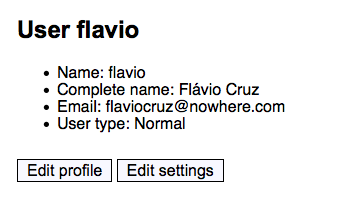
\includegraphics[scale=0.6]{settings.png}
  \caption{Page with user information.}
  \label{fig:settings}
\end{figure}

Selecting \textbf{Edit profile} enables us to edit the complete name, email or password.
When editing any information here, you should input your old password. If you want to change
the current password fill the two text fields for that, if not, leave them empty.

The other button, \textbf{Edit settings} enables you to change other, aspect related settings, like
the number of items per grid.

\subsubsection{Managing other users}

If you are an administrator using the \textbf{admin} account, you can edit other user profiles,
through \textbf{Administration - Users - List} and then selecting the target user. When editing
one user you should enter the \textbf{admin} password and not the user's current password.

For some reason, if you want to disable one user, go to the users list, select the user name
and click the \textbf{Delete} option.

One very destructive feature is the \textbf{Database reset}. It
can be accessed through the menu option \textbf{Administration - Reset Database} and removes all
custom data from the database, which is:

\begin{itemize}
  \item All taxonomy trees, except the NCBI tree.
  \item All ranks except the system defaults.
  \item All non-default labels.
  \item All sequences.
  \item All normal users.
  \item All files in the \textbf{file} table.
\end{itemize}

\subsection{Import / Export database}

Another useful feature is the database export / import facilities. One can
export the whole database as a XML file and then import it somewhere else, literally copying
the source database.

What is exported?

\begin{itemize}
  \item labels
  \item ranks
  \item taxonomy trees, except the NCBI tree
  \item sequences
\end{itemize}

To export the database, use the option \textbf{Administration - Export Database}.

To import a database XML file, go to \textbf{Administration - Import Database} from
the main menu. There you should upload the file and, once processed, an import report
is shown. The report is similar to the individual ones, but over various entities.

\subsection{Application customization}

There are two ways of customizing the application:

\begin{itemize}
  \item Changing the text that appears on the header: use the option \textbf{Administration - Database Description}.
  \item Changing the application's background: use the option \textbf{Administration - Database Background}. You should upload an JPG or PNG file.
\end{itemize}


\chapter{Tables}\label{app:tables}

\begin{table}[ht]
  \begin{tabular}{ | >{\centering}m{20mm} | p{12cm} |}
    \hline
    Table & Fields \\ \hline
    User & \begin{itemize}
      \item id (SERIAL)
      \item name (CHAR)
      \item complete\_name (VARCHAR)
      \item password (CHAR): MD5 hash of the user password. 
      \item email (VARCHAR)
      \item user\_type (ENUM): Can be 'admin' or 'user'.
      \item enabled (BOOL): TRUE if user is active.
      \item history\_id (ID): Pointer to history table.
      \item last\_access (TIMESTAMP): Timestamp of last access.
    \end{itemize} \\ \hline
  \end{tabular}
  \caption{User table.}
  \label{tbl:user_table}
\end{table}

\begin{table}[H]
  \begin{tabular}{ | >{\centering}m{25mm} | p{12cm} |}
    \hline
    Table & Fields \\ \hline
    Configuration & \begin{itemize}
      \item user\_id (ID): Pointer to user table.
      \item key (CHAR)
      \item value (VARCHAR)
    \end{itemize} \\ \hline
  \end{tabular}
  \caption{Configuration table.}
  \label{tbl:configuration_table}
\end{table}

\begin{table}[H]
  \begin{tabular}{ | >{\centering}m{20mm} | p{12cm} |}
    \hline
    Table & Fields \\ \hline
    History & \begin{itemize}
      \item id (SERIAL)
      \item creation\_user\_id (ID): Pointer to user who created the object.
      \item creation (TIMESTAMP): Timestamp at creation's time.
      \item update\_user\_id (DI): Pointer to user who made the last object update.
      \item update (TIMESTAMP): Last update's timestamp.
    \end{itemize} \\
    \hline
  \end{tabular}
  \caption{History table.}
  \label{tbl:history_table}
\end{table}

\begin{table}[H]
  \begin{tabular}{ | c | p{12cm} |}
    \hline
    Table & Fields \\ \hline
    TaxonomyNameType & \begin{itemize}
      \item id (SERIAL)
      \item name (VARCHAR)
    \end{itemize} \\ \hline
  \end{tabular}
  \caption{TaxonomyNameType table.}
  \label{tbl:taxonomy_name_type_table}
\end{table}

\begin{table}[H]
  \begin{tabular}{ | c | p{12cm} |}
    \hline
    Table & Fields \\ \hline
    TaxonomyName & \begin{itemize}
      \item id (SERIAL)
      \item name (VARCHAR)
      \item tax\_id (ID): The taxonomy this name refers to.
      \item type\_id (ID): Points to a TaxonomyNameType row.
    \end{itemize} \\ \hline
  \end{tabular}
  \caption{TaxonomyName table.}
  \label{tbl:taxonomy_name_table}
\end{table}

\begin{table}[H]
  \begin{tabular}{ | c | p{12cm} |}
    \hline
    Table & Fields \\ \hline
    TaxonomyRank & \begin{itemize}
      \item id (SERIAL)
      \item name (CHAR)
      \item history\_id (ID): To store rank history information.
      \item parent\_id (ID): Pointer to parent rank.
      \item is\_default (BOOL): TRUE if system rank.
    \end{itemize} \\ \hline
  \end{tabular}
  \caption{TaxonomyRank table.}
  \label{tbl:taxonomy_rank_table}
\end{table}

\begin{table}[H]
  \begin{tabular}{ | c | p{12cm} |}
    \hline
    Table & Fields \\ \hline
    TaxonomyTree & \begin{itemize}
      \item id (SERIAL)
      \item name (VARCHAR)
      \item history\_id (ID): To store tree history information.
    \end{itemize} \\ \hline
  \end{tabular}
  \caption{TaxonomyTree table.}
  \label{tbl:taxonomy_tree_table}
\end{table}

\begin{table}[H]
  \begin{tabular}{ | c | p{12cm} |}
    \hline
    Table & Fields \\ \hline
    Taxonomy & \begin{itemize}
      \item id (SERIAL)
      \item name (VARCHAR): Taxonomy's main name.
      \item parent\_id (ID): Pointer to parent taxonomy in this table.
      \item rank\_id (ID): Taxonomy rank.
      \item tree\_id (ID): The tree where this taxonomy belongs.
      \item history\_id (ID): To store taxonomy history information.
      \item import\_id (ID): ID in the imported database.
      \item import\_parent\_id (ID): Parent ID in the imported database.
    \end{itemize} \\
    \hline
  \end{tabular}
  \caption{Taxonomy table.}
  \label{tbl:taxonomy_table}
\end{table}

\begin{table}[H]
  \begin{tabular}{ | c | p{12cm} |}
    \hline
    Table & Fields \\ \hline
    Label & \begin{itemize}
      \item id (SERIAL)
      \item type (ENUM): Can be: integer, float, text, obj, position, ref, tax, url, bool or date.
      \item name (CHAR)
      \item comment (VARCHAR)
      \item history\_id (ID): To store label history information.
      \item default (BOOL): If true, label is a system label.
      \item must\_exist (BOOL): If true, each sequence must have an instance of this label.
      \item auto\_on\_creation (BOOL): If true and when a sequence is being added into the system, a label instance should be generated and connected to the new sequence.
      \item auto\_on\_modification (BOOL): If true and when a sequence content is being modified, the label instance should be edited and auto generated.
      \item code (TEXT): Code run to create a new label instance.
      \item valid\_code (TEXT): Code run to valid a label instance value.
      \item deletable (BOOL): If true, the user can delete the label instances.
      \item editable (BOOL): If true, the user can manually modify the label instances.
      \item multiple (BOOL): If true, a sequence can have multiple instances of this label, only if they are distinguished by a parameter string.
      \item public (BOOL): If true, this label can be used in public searches.
      \item action\_modification (TEXT): Code that is run when a sequence having label instances is modified.
    \end{itemize} \\ \hline
  \end{tabular}
  \caption{Label table.}
  \label{tbl:label_table}
\end{table}

\begin{table}[H]
  \begin{tabular}{ | c | p{12cm} |}
    \hline
    Table & Fields \\ \hline
    Sequence & \begin{itemize}
      \item id (SERIAL)
      \item content (MEDIUMTEXT): The sequence content.
      \item name (CHAR)
      \item history\_id (ID): To store sequence history information.
    \end{itemize} \\ \hline
  \end{tabular}
  \caption{Sequence table.}
  \label{tbl:sequence_table}
\end{table}

\begin{table}[H]
  \begin{tabular}{ | c | p{12cm} |}
    \hline
    Table & Fields \\ \hline
    LabelSequence & \begin{itemize}
      \item id (SERIAL)
      \item seq\_id (ID): Sequence pointer.
      \item label\_id (ID): Label pointer.
      \item history\_id (ID): To store instance history information.
      \item int\_data (INT)
      \item text\_data (VARCHAR)
      \item obj\_data (ID)
      \item ref\_data (ID)
      \item position\_start (INT)
      \item position\_length (INT)
      \item taxonomy\_data (ID)
      \item url\_data (VARCHAR)
      \item bool\_data (BOOL)
      \item date\_data (DATETIME)
      \item float\_data (DOUBLE)
      \item param (TEXT): Used to distinguish between multiple label instances.
    \end{itemize} \\
    \hline
  \end{tabular}
  \caption{LabelSequence table.}
  \label{tbl:label_sequence_table}
\end{table}

\begin{table}[H]
  \begin{tabular}{ | >{\centering}m{20mm} | p{12cm} |}
    \hline
    \textbf{Table} & \textbf{Fields} \\ \hline
    Event & \begin{itemize}
    \item id (SERIAL)
    \item code (int): Event code.
    \item data (text): Event information.
    \end{itemize} \\ \hline
  \end{tabular}
  \caption{Event table.}
  \label{tbl:event_table}
\end{table}

\begin{table}[H]
  \begin{tabular}{ | >{\centering}m{20mm} | p{12cm} |}
    \hline
    \textbf{Table} & \textbf{Fields} \\ \hline
    File & \begin{itemize}
      \item id (SERIAL)
      \item label\_id (ID): Which label this file refers to.
      \item name (VARCHAR): File name.
      \item count (INT): Reference count.
      \item data (LONGBLOB): File data, the file itself.
      \item type (TEXT): Optional field to indicate the file type.
    \end{itemize} \\ \hline
  \end{tabular}
  \caption{File table.}
  \label{tbl:file_table}
\end{table}

\end{document}
